\documentclass[nomlist,masters,openany]{seuthesix}
\usepackage{multirow}
\usepackage{amsmath} 
\usepackage{booktabs}
\begin{document}
\categorynumber{TP311} % 分类采用《中国图书资料分类法》
\UDC{004.4}            %《国际十进分类法UDC》的类号
\secretlevel{公开}    %学位论文密级分为"公开"、"内部"、"秘密"和"机密"四种
\studentid{141466}   %学号要完整,前面的零不能省略。
\title{\quad}{基于本体的地理知识问答}{\quad}{Ontology-based Geographic knowledge question answering}
\author{张赏}{Wu Zhanpeng}
\advisor{高志强}{教授}{Gao Zhiqiang}{Prof.}
%\coadvisor{楚留香}{副教授}{Perfume Tsu}{Associate Prof.} % 没有% 可以不填
 \degreetype{工程硕士}{Master of Engineering} % 详细学位名称
\major{计算机科学与技术}
\submajor{计算机技术}
\defenddate{2017年5月31日}
\authorizedate{20~~~~年~~月~ ~日}
\committeechair{陈国庆}
\reviewer{张志政~教授}{匿名评阅人}
\department{计算机科学与工程学院}{School of computer science and engineering}
\seuthesisthanks{本工作受到国家自然科学基金61170165、61602260和61502095的资助。}
\makebigcover
\makecover
\begin{abstract}{地理高考,本体,知识库问答,双向长短期记忆网络,注意力机制}
	在人工智能领域,自动解答高考题是一项很具挑战性的任务。与一般事实性问答的问题不同,高考题带有很强的选拔性。其问题考察形式多变,其答案求解往往不能一步得到,通常需要做进一步的知识推理。在辅助解答高考地理题时,目前面临两个问题:第一是缺乏高度结构化的地理核心知识库。高考地理题的考点专业性很强,考点知识大都来自地理教科书章节知识,然而地理教科书是以文本文档的形式存在,无法准确表示出地理知识点之间的语义层次关系,因而也不适合当作计算机解答高考地理题的核心知识库。第二是地理问题表达形式多样,导致问题理解困难。地理问题中往往包含大量的无效信息,这些信息极易淹没问题核心考点信息,因而很难从大量干扰信息中精准地找出问题考点。针对以上问题,本文作了如下工作:
	
	(1)为解决高度结构化的地理核心知识库缺乏问题,本文构建了中文地理本体(Chinese Geographic Ontology, CGeoOnt)知识库(Knowledge Base, KB)。该本体知识库以人教版高中地理教科书为知识源,使用万维网本体语言(Web Ontology Language, OWL)为知识表示语言,以课本章节为知识体系,人工总结其核心地理概念、地理关系、地理考点,并将其表示为本体形式。同时,本文将构建的CGeoOnt与本体知识库Clinga进行本体融合,得到一个更大规模的中文地理本体知识库。
	
	(2)为解决地理问题问法多样导致其难以理解问题,本文使用基于神经注意力机制的知识库问答模型。该模型以双向长短期记忆网络为基础问答模型,结合注意力机制对答案进行表示,答案中每个词的向量生成,均结合其对问题各词的注意力权重分配,使答案可以更好的对齐问题中关键信息,减弱无效信息的干扰,因此更易区分正确答案和错误答案。实验表明,该问答模型对于辅助解答地理高考题具有很好的应用价值。
	
	(3)为解决中文地理问答模型在训练和测试中数据集缺失问题,本文从互联网收集了一个问法多样的中文地理问题集。本文使用百度问题推荐以及百度搜索API,以本体知识库高频核心知识三元组为数据源,依次访问到二十万个Web地理问题,然后半自动加人工挑选出其中的有效问题,形成最终数据集。
\end{abstract}
\begin{englishabstract}{Entity Linking, Active Learning, Corpus Construction}
	Entity linking is the task of determining the identity of entities mentioned in text. Supervised learning approaches and unsupervised learning approaches have been widely used in entity linking task in the past decade. However, only a few studies have been reported on accelerating model training and improving corpus construction. Active learning can contribute to interactively obtain optimum samples and provide them for annotators to conduct manual annotation according to the learning process. Meanwhile, it can reduce the quantity of the training samples as well as keep or improve model performance.
	
	This thesis analyzes the characteristics of entity linking task, and use active learning approaches to handle model training and corpus construction task based on active learning.
	
	The main contributions of this thesis include two aspects as follow:
	
	(1) In consideration of supervised learning model of entity linking, this thesis reduces human annotating effort by using active learning, and proposes two approaches. One is an initial sample selection approach based on popularity, as known as sampling by popularity (SBP). The other is an iterative training sample selection approach based on comprehensive uncertainty and popularity, as known as sampling by uncertainty and popularity (SUP) . This way ensures representative of initial training sample in the initial sample selection stage and considers both uncertainty and representative of selected samples in the following stage of iterative sample training.
	
	(2) To construct entity linking corpus, this thesis proposes an annotating approach based on active learning and unsupervised learning for improving annotation quality. In this way, the most informative samples of unlabeled mentions can be found for annotators to annotate while the precision rate of the whole corpus can be improved by propagating the evidence of labeled mentions.
	
	Experiments in this thesis show two main points. One is that approaches of SBP and SUP can effectively accelerate the training process of entity linking model. The other is that approaches of annotation based on active learning and unsupervised learning can effectively improve the accuracy of annotating a silver-standard entity linking corpus on the premise of annotating fewer mentions.
\end{englishabstract}

\setnomname{术语与符号约定}
\tableofcontents
\listofothers

\mainmatter

\chapter{绪论}
\section{研究背景}
近年来,一个比较热的人工智能挑战是让计算机通过高考。早在2011年,日本国立情报学研究所(NII)发起了一项名为“东大机器人项目”(Todai RobotProject)的人工智能项目,其最终目的是让此名为“Torobo”的“高考机器人”能够在2021年通过东京大学的入学考试\cite{Fujita}。在2015年,国家也启动了863“基于大数据的类人智能关键技术与系统”项目,其目的为攻克高考九门学科中的四门,即语文、数学、地理、历史\cite{Cheng}。本文工作也是对辅助解答地理高考多选题的一些尝试,图1所示为2016年上海地理高考多选题:

\begin{figure}[!htb]
	\centering
\includegraphics[height=2.2cm]{resource/ex_multi_choice_ques}
	\caption{地理高考多选题举例}
	\label{fig:ex_multi_choice_ques}
\end{figure}

题中划线部分为此题问题,划线部分之前为问题的背景知识介绍。由题可知,问题考察“厄尔尼诺现象会使哪些国家或地区产生干旱现象?”,要解答此问题,计算机必须具备“厄尔尼诺现象”相关的核心知识。如此处需要知道地理知识,厄尔尼诺现象使印度、东南亚、印度尼西亚和澳大利亚产生干旱,然后根据选项中“泰国”属于东南亚,可得此题答案选“泰国”。由上述解题过程可知,解答此类地理问题需要高度结构化的地理知识,并且知识表示需包含丰富的语义信息。如此题需要知道“(厄尔尼诺现象,导致干旱的国家,印度、东南亚、印度尼西亚、澳大利亚)”三元组,同时也需要知道“(东南亚,包括,越南、老挝、柬埔寨、缅甸、泰国、马来西亚、新加坡、印度尼西亚、菲律宾、文莱、东帝汶)”,并且我们还需要知道“东南亚”的类别是一些国家的集合,“泰国”的类别属于东南亚国家。

鉴于以上分析,解答高考地理题多选题一般包含两步,第一步为匹配求解问题所需的知识库三元组知识,第二步为根据结果三元组作进一步推理得出最终答案。作为辅助解答高考地理选择题,本文的工作集中在第一步上,即先构建解答地理高考题所需要的地理核心知识库,再从该知识库中找出最可能回答所求地理问题的知识三元组。

地理解题核心知识库需要高度结构化的知识表示,并且知识需包含丰富的语义信息,如知识类别、关系等。显然,无结构的文本文档以及半结构化的数据(如xml、json格式)表示形式都无法满足要求。在结构化表示领域知识时,本体可以很好对领域知识建模,并且表示出计算机可以处理的带有丰富语义的形式化定义\cite{Hitzler}。前期的地理知识以地理教科书形式存在,地理教科书知识分章节层次描述,计算机是无法处理此自然语言式的语义关系。因此需要使用本体对其建模,通过本体中的实体、类别、属性、关系等术语,描述地理中概念(如地球、星球等)的属性信息,描述概念的类别信息,描述各概念之间的相互作用关系。地理核心知识通过三元组(主、谓、宾形式元祖)形式得以更精炼的表示,地理核心概念层次关系明显,更适合作进一步的推理。

基于构建的地理核心知识库之上,本文需要构建一个问答系统。给定一个地理问题,系统需返回求解该问题所需的地理知识三元组。目前,基于知识库的问答任务有两个主流的研究方向:基于语义解析\cite{Zettlemoyer,Cai,BerantCA,Dyer}和基于信息检索\cite{Yao,Bordes1,Dong,Bordes2}。基于语义解析的方法一般先构建一个语义解析器, 然后运用该语义解析器将自然语言问句转换为特定类型的逻辑表达式,如带类型的 lambda 表达式(typed lambda calculus)、 lambda 依存组合语义\cite{Wong,BerantCA,Yih}。基于信息检索的方法通常先从知识库检索一系列候选答案,然后对问句和候选答案进行特征抽取并打分,选出得分最高的结果作为最终答案\cite{Bordes1,Kim}。基于信息检索的方法更简单,实现也更灵活,在开放域知识库Freebase上的问答实验表明,该方法可以达到与基于语义解析方法相近的 F 值\cite{Dong,Bordes2}。随着深度学习的兴起,神经网络被运用到知识库问答中提升已有模型,基于神经网络的模型只需将问题和答案分别表示成语义向量,然后计算向量相似性即可获得最相似的候选答案。问句和答案的向量表示是基于神经网络模型的一个重要环节,有些研究比较侧重答案表示,如运用候选答案在知识库子图中的重要性\cite{Bordes1}或者答案的类型和上下文\cite{Dong}。这些研究往往使用简单的词袋模型来表示问题,忽视了问题与答案的关联性\cite{Bordes1}。还有研究使用Attention机制根据不同答案的不同注意力方面来表示问题\cite{Zhang},取得了比较好的效果。

分析本文搜集到的地理问题可知,地理问题表达形式多样,无效信息较多,一个地理三元组往往可以成为多个问题的答案。如三元组——“(季风气候,生产优势,夏季高温多雨、雨热同期)”,可以作为“亚热带季风气候在发展农业生产方面有什么优势” 和“温带季风气候在农业生产方面的显著优势是\_百度知道”这两个问题的答案。虽然两个问题在问题表述不一样,但其问题核心均考察“季风气候的生成优势”,因此相对答案三元组而言它们是等效的。这也说明,在我们做问答时,单独的表示问题和答案向量是不准确的,至少是不能表示问题和答案之间关系的,因此可以结合Attention机制,在答案向量表示时同时结合对问题的Attention权重,这样可以更合理的表示问题和答案的关系,同时答案中重要信息可以与问题中重要信息对齐,这样也减弱了问题中无效信息的影响,可以获得更好的问答效果。

\section{研究内容}
本文为辅助解答高考地理多选题所做的工作,本文核心内容为从构建的地理核心知识库中找出可以回答所求地理问题的知识三元组。因此,本文研究如何使用本体更准确、更精炼地表示地理教科书中的知识,从而构建一个高质量、高可用性的地理知识库。同时,本文研究如何更准确的根据表达形式多样的地理问题,从构建的地理知识库中找出可以回答该问题的地理知识三元组,便于解题组根据此三元组作进一步的答案推理,得出问题最终答案。

本文主要研究内容如下:

(1)为解决高度结构化的地理核心知识库缺乏问题,构建了中文地理本体CGeoOnt知识库。本体知识库的构建使用OWL本体语言,将地理教材中的核心考点概念属性、核心概念之间的关系形式化表示。并且,运用启发式规则将CGeoOnt与本体Clinga进行融合,采取人工做最终的融合校验,形成更综合的中文地理本体知识库。

(2)为解决地理问题问法多样导致其难以理解问题,使用基于神经注意力机制的双向长短期记忆内存网络知识库问答模型。问答模型不是独立对问题和答案进行词向量表示,而是在充分考虑问题和答案之间的依赖关系基础上,结合问题对答案进行综合词向量表示。使正确答案三元组与问题关键信息对齐,减弱非关键信息的干扰,从而更易区分相近的答案三元组,使模型辨别答案能力更强。

(3)为解决中文地理问答模型在训练和测试中数据集缺失问题,从互联网收集了一个问法多样的中文地理问题集。问题集中的问题知识均来自地理知识库中的核心出题考点,运用百度问题推荐和问题搜索API,从互联网获取这些考点的相关地理问题,经机器半自动筛选和人工筛选出有效的问题。最后,人工从本文构建的地理知识库中选择能回答这些问题的三元组知识,形成最终的问题、答案对数据集。

\section{论文组织}
本文共分为五章,各章的主要内容如下:

(一)第一章主要介绍相关的基本概念、应用背景,以及研究内容和论文的组织结构。

(二)第二章主要介绍实体链接任务和主动学习方法的研究现状。介绍了实体链接任务的基本概念以及常用的处理方法,分析了目前实体链接任务方法各自的优缺点;还介绍了主动学习方法的概念、常用的方法、以及它在其它机器学习任务中的应用。

(三)第三章首先介绍基于主动学习的实体链接模型的训练方法。然后介绍经过改进的主动学习方法,提出了基于流行度的初始样本选择方法以及综合不确定度和流行度的迭代训练样本选择方法。并通过实验验证了本文所提方法的有效性。

(四)第四章首先介绍基于主动学习的实体链接银标准语料构建方法。然后提出待标注样本的选择方法,以及标注结果的证据传播方法。并通过实验验证银标准语料库构建效率的提升效果。

(五)第五章对全文进行总结,指出本文的创新点和不足之处,并对未来的研究进行展望。


\nomenclature{EL}{Entity Linking}
\nomenclature{NER}{Named Entity Recognition}
\nomenclature{AL}{Active Learning}
\nomenclature{SBP}{Sampling by Popularity}
\nomenclature{SUP}{Sampling by Uncertainty and Popularity}
\nomenclature{RW}{Random Walk}
\nomenclature{EP}{Evidence Propagation}

\chapter{相关研究}
本章介绍本文相关研究工作,主要包括本体和问答的研究现状。首先介绍本体相关内容,包括本体核心构成要素:个体、类、属性、关系和本体描述语言;然后介绍知识库问答的主流方法,包括基于语义解析的方法和基于信息检索的方法;最后介绍本文的工作特色。

\section{本体构成要素}
从计算机科学角度看,本体是对相关领域知识的一种高度结构化、层次化的抽象建模,这种建模表示包含一系列计算机可以处理的形式化定义\cite{Hitzler}。运用本体可以很好的表示出领域中核心概念的语义信息和概念之间的相互关系。通过4个核心要素个体(Individuals)、类(Classes)、属性(Properties)及关系(Relationships),本体能够将领域知识以一种类似现实世界的组织方式形式化的表示出来,并且从某种程度上,既符合人的直观对领域知识层次分类的理解,又适合计算机存储、检索和推理。因此,本体是一种很好的结构化知识库建模方式。

\subsection{个体(individuals)}
个体,又叫实例(instances),是本体中最基本、最底层的组成单元。本体大多数描述都是企图更准确、更详细的描述出个体的信息特征。常见的人、动物、汽车、天体、星球等中的具体对象都可以看做个体(如地球、月球、太阳都是个体),就算是抽象的数字、单词等也可以视作个体。本体的一个很重要任务就是对本体领域中的个体进行层次化的分类,使得不同个体可以很好的进行区分或者是使其可以建立某种关联。

\subsection{类(classes)}
类,又叫类型(type)、类别(sort)、种类(kind)或者类目(category),常常指某个个体的上层延伸或者内涵。类是一些特征相似的个体构成的一个集合,或者是有一些子类构成的大类集合。如下为类的举例:

(1)人:人包括黄种人、白种人等类型,具体的张三、李四也是人的个体。

(2)动物:动物包括无脊椎动物和脊椎动物两大类。

(3)汽车:汽车表示所有具体品牌汽车的类别。

(4)天体:天体包括地球、月球、彗星、流星等宇宙空间的物质。

(5)行星:行星包括地球、金星、木星、水星、火星、土星、天王星、海王星等。

通常情况下,一个个体可以属于不同的类别,这样使表达更灵活、表达力更强。同时,一个类可以包含其他类或者被其他类包含,这样构成了类的层次关系。一个类A被另一类B包含称为:A \textit{is subClassOf} B,通过这个关系可以得到很重要的性质,即B类具有的性质A类也同样具有。同样,一个类可以被多个类包含,也就是说一个类可以有多个父类。正是类别的上述层次关系,使知识不仅可以表示其自身的特征,还可以表示其与其它知识的关系,而且这种关系是非常接近人类的概念思维,所以知识建模非常直观。

\subsection{属性(Properties)}
属性用于表示个体间的关系(ObjectProperty)或者个体与其数据值之间的关系(DatatypeProperty)。例如人相关的属性\textit{hasWife}、\textit{hasHeight}和\textit{hasAge},\textit{hasWife}表示两个人(两个具体的人是两个个体)之间是夫妻关系,\textit{hasHeight}和\textit{hasAge}表示一个人的身高和年龄,身高、年龄值为数值类型。同样,属性与类结构类似,具有子属性层次结构。

属性的另外一个重要特点是,属性含有定义域(domain)、值域(range)的限制(restriction)。运用属性的这一限制,可以对属性两边的个体做相关的类别推理。如根据申明两个个体是\textit{hasWife}关系,可以推导出这两个个体的类别都是人,且更进一步该关系左边的个体类别为男人,右边的个体类别为女人。

\subsection{关系(Relationships)}
关系用来表示对象之间是以怎样的方式相联系在一起的。以汽车系列举例:“福特探险者是福特野马的下一代”,此例子体现出“福特探险者”和“福特野马”这两个对象存在着“下一代”的关系,这一事实可以表示为:

\begin{center}
	“福特探险者 \textit{is defined as a successor of} 福特野马”
\end{center}

此关系表达出“福特探险者系列”取代了“福特野马系列”这一事实,显然这种关系是存在着方向的。同样可以用此关系的反向关系,即“上一代”来表示上面的事实——“福特野马是福特探险者的上一代”。关系的总集合就构成了领域本体的丰富语义信息,因此关系的表达能力大小很大程度决定着本体对领域的抽象建模能力。如下介绍两种重要的关系:

(1)包含关系(subsumption relation)

包含关系主要有\textit{is-a-superclass-of}、\textit{is-a-subclass-of}和\textit{is-a-subtype-of},分别表示父类关系、子类关系和子类型关系。这些关系都是表达一种上下位的关系,特别是其中的\textit{is-a-subclass-of}关系,它体现出一中很强的分类学思想,可以直观地对领域概念进行分类,并且表示出这些类别的层次关系。

(2)总分学关系(mereology relation)

总分学关系指的是一种部分(\textit{part-of})与整体的关系,表示一个对象是另一个复合对象的一部分。还是以“福特探险者”系列为例,“方向盘 \textit{is-a-part-of} 福特探险者”,表示方向盘是福特探险者汽车的一个部件。

除了包含关系和总分学关系以外,本体中还有一些其它的关系,这些关系不一定表示层次关系,其往往是该本体领域中的特定业务关系。这种领域的特定关系被用来表达领域独特的事实知识,构成了自身领域本体的特色,因此不同领域本体表示往往差别比较明显。

\section{本体描述语言}
使用本体描述语言可以很好的对领域本体进行层次化的表示。常见的本体描述语言有:Ontolingua、OCML、OKBC、FLogic、LOOM、DAML、SHOE, OIL、XOL、XML、RDF、RDFS、OWL\cite{Corcho}。其中,由W3C推荐的XML、RDF、RDFS以及OWL使用最为广泛。

XML(Extensible Markup Language)\cite{xml}是一种标记语言,通过其标记可以对结构化文档进行分层的语法表示,并且易于机器处理和人类阅读。然而,XML标记缺乏对文档的含义进行约束,标记内部也缺乏结构化定义,因此很难充分描述出本体中的四个常见核心要素。RDF(Resource Description Framework)\cite{rdf}是一种描述对象(资源)以及对象之间关系的图数据模型,其兼容XML语法,并且含有简单的语义。RDFS(RDF Schema)\cite{rdfs}是扩展的RDF词汇表,这里的词汇表指定义为个体、类、属性和关系的术语名称。RDFS通过扩展了RDF中没有的属性和类层次结构语义,也即通过定义子属性(subPropertyOf)、子类(subClassOf)、属性定义域约束、属性值域约束来增强描述资源的表达能力。尽管RDFS相对RDF的描述资源能力更强,RDFS仍然是一种相对简单的本体语言,其描述资源能力依然很有限\cite{gao}。例如:RDFS无法描述类的不相交关系,如类“男人”和“女人”是不相交的,但其只能描述“男人”和“女人”同属于“人”;同时,RDFS也无法描述类的布尔组合(并集、交集、补集)关系,如“人”无法定义成“男人”和“女人”的并集等。为弥补RDFS表达能力的不足,W3C又推出了表达能力更强且具备强推理能力的本体语言——OWL(Web Ontology Language)\cite{owl},OWL定义了逻辑类的关系表示,即提供了针对逻辑与、或、非的领域关系表示,可以有效的表示类的并集、交集、补集运算,因而可以表达更复杂的本体知识。

OWL的一个很重要设计思想是在知识的表达能力和推理效率之间找到一个平衡。因此,在其不同的表达能力和推理效率设计中,为了满足不同用户对本体的建模需求,又诞生了三个子语言,即OWL Lite、OWL DL(Description Logic)和OWL Full。这三个子语言描述能力依次增强,推理复杂度也逐渐提高。OWL Lite更关注本体表达的简洁性,其表达能力相对其它两种语言较弱,但它的推理最高效,因此OWL Lite更适合于对表达能力要求不是太强的领域;OWL DL比OWL Lite表达能力更强,与OWL Full比具有计算完备性(所有结论均可计算)和可判定性(有限时间内所有计算均可终止),同时OWL DL支持有效的推理,因此在既对本体语言表达能力要求高,又需要保证推理的可判定性情景时,可以选择此本体语言;OWL Full在这三种语言中表达能力最强,正因其表达更灵活、约束较少,也使其推理不可判定,但OWL Full有完全兼容RDF的优点,这也是前两种语言不具备的,因此在以兼容RDF为主要建模目标的场景,OWL Full语言是不错的选择。

\section{本体构建方法}
目前,本体构建方法\cite{yue}主要有两种:第一种是在领域专家的指导下,使用本体描述语言表示领域本体;第二种是从结构化、半结构数据或者无结构文本中抽取本体要素,从而形成领域本体。第一种本体构建方法往往采用纯手工方法,由于人的主观性,不同领域专家构建出来的本体常常相差很大、
且构建效率低。但从局部来看,专家构建的本体知识质量很高,因为专家站在领域的高度对繁杂的知识进行了专业化的总结、提炼,使知识表达更专业所以,在对知识表示专业程度、准确程度要求很高但知识数量比较小的领域(如高考地理解题核心考点本体),此方法可以达到很好的效果。第二种本体构建方法是为了缓解第一种方法中的人为主观性和低效性而提出的,其使用自动或者半自动的方法构建本体,既节省了时间又提高了本体知识表示的一致性。第二种本体构建方式很大程度依赖于自动或者半自动技术的能力,构建出来的本体往往噪音较多、抽象程度不高(知识没有经过深度提炼、总结)。因此,在一些对知识准确度要求很高的场景,如地理高考解题本体构建等,此方法不是很适合,但是在一些对噪音容忍度比较高的场景,如通用领域的本体构建,此方法运用很广且效率很高。

由于本文构建用于解答高考地理题的地理本体,其知识要求精炼、准确、少噪音且知识量不大(只构建核心地理高考考点),因此需要地理领域相关工作人员人工构建,保证质量。本文也只详述人工本体构建的研究现状,对于自动和半自动本体构建方式的研究现状,本文不加以叙述。

国内外常见人工本体构建方法有:IDEF5法\cite{IDEF5}、骨架法\cite{skelton}、TOVE法\cite{TOVE}、METHONTOLOGY法\cite{METHONTOLOGY}、KACTUSK工程法\cite{KACTUSK,KACTUSK2}、SENSUS法\cite{SENSUS}以及七步法\cite{seven}等。IDEF5法、骨架法及TOVE法常用于企业领域本体构建。IDEF5法使用图表以及很细化的说明形式来获取企业业务存在的概念、属性及关系,从而形成本体;骨架法是一种流程图导向的本体构建方法,其描述的是一种本体构建的方法框架;TOVE法是通过本体建立企业知识的逻辑(一阶逻辑)模型。其它四种方法用于构建领域知识本体。METHONTOLOGY法是在构建化学元素周期表本体基础上发展而形成的通用本体构建方法,此方法偏向软件工程的思想,本体的构建也引入了管理、开发和维护三个很具软件工程特征的阶段;KACTUS法是对应用驱动的本体开发方法,侧重对已有本体的复用和扩充方法;SENSUS法提供一种自顶向下的层级结构本体构建方法,偏向操作性指导。七步法是基于本体工具protege\footnote{https://protege.stanford.edu/}的构建方法,主要分七个步骤构建本体,比较偏向实用性、操作性。具体七种本体构建方法比较如表3.4.1所示

\begin{center}
	\begin{small}
	表3.4.1 七种本体构建方法比较
	\end{small}

\end{center}

\begin{figure}[!htb]
	\centering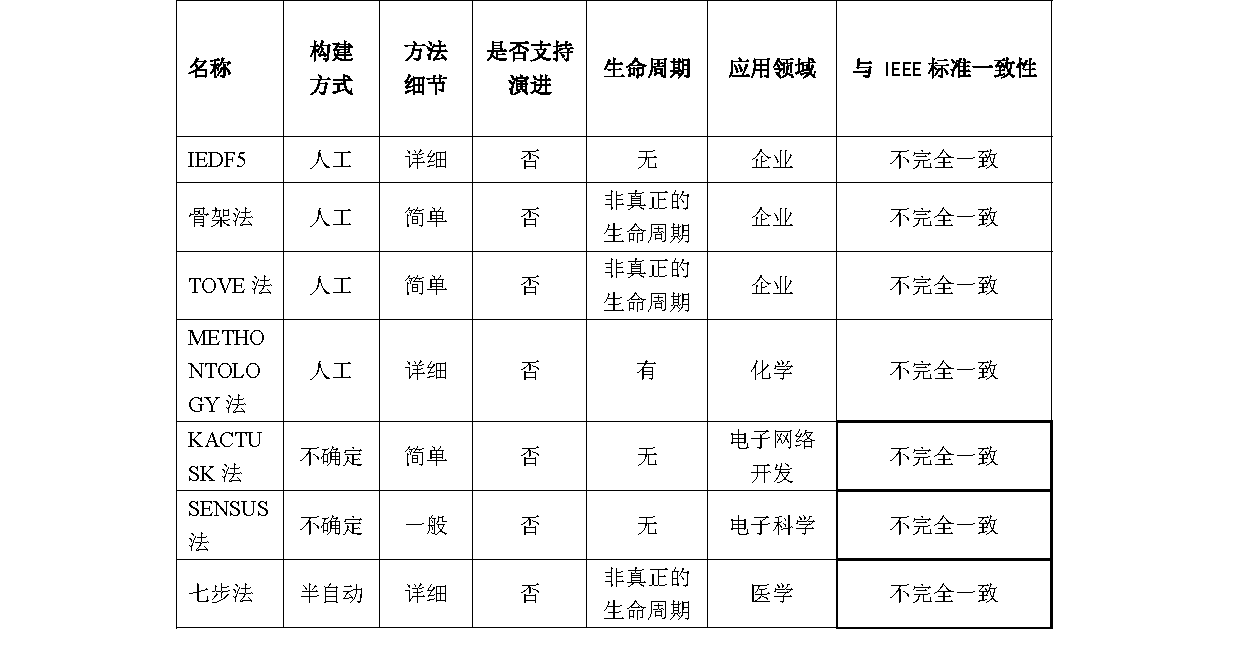
\includegraphics[height=7cm]{resource/onto_method_compare}
	\label{fig:onto_method_compare}
\end{figure}

分析以上七种人工本体构建方法可知,这些构建方法都缺乏对本体进化的考虑,本体只立足当下情况,没有考虑后期本体的更新,也使本体知识不能与时具进。同时,这些方法人工参与力度很大,使用的技术较简单,构建时并没有统一的标准规范对其指导,构建人员均需从自身领域特点出发进行扩展与缩减。因此,本体构建的不统一性还是比较大,这也表明统一的本体构建规范,评价标准还不成熟。

\section{问答方法研究}
问答是人工智能领域中的一个热门的研究问题,它综合运用了各种自然语言处理技术。对于用户提出的某一个问题,问答系统往往可以给出简短、精准的答案组织形式,而非一系列的相关网页文档供用户参考,省去了用户额外从大量的相关网页文档中寻找所需确切信息的时间\cite{Lu} \cite{Bertola}。同时,问答技术集成了定位,抽取以及表示出针对用户提出的自然语言问题答案的丰富功能,因此受到广泛的关注\cite{Abacha}\cite{Pavli}。

问答一般分为两类:开放域的问答和封闭域的问答。开放域的问答又叫无结构数据的问答,一般是从开放的网页或者文档中抽取所需的问题信息。封闭域的问答又叫受限域的问答或结构化数据的问答,其往往需要预先定义的知识源,例如领域本体或关系数据库管理系统\cite{Dalmas}\cite{Dragoni}. 查询数据库的方式有两种,第一种为结构化查询,如SQL,另一种为自然语言查询,即用户用自然语言组织其问题而不需要一些专业术语的限制\cite{Jagadish}。结构化查询虽其功能强大,但不易使用,对缺乏训练的普通用户不友好。相反,自然语言查询方式对用户更友好,用户可以轻松组织自然语言进行复杂的问题查询。

对于知识问答而言,其强调如何根据给定问题作出精准回复,其答案要求不能包含无效的信息。因此,知识问答的知识源常常选取高度结构化、包含丰富语义信息的数据,如本体等。建立于高度结构化数据之上的问答也叫做知识库问题,本文将详述知识库问答的主流研究方向和方法。

目前,知识库问答(knowledge base question answering,KBQA)主要有两个主流的研究方法:基于语义解析、基于信息检索。分别如下介绍:

\subsection{基于语义解析的KBQA}
基于语义解析的方法一般先构建一个语义解析器,然后运用该语义解析器将自然语言问句转换为特定类型的逻辑表达式,如带类型的 lambda 表达式(typed lambda calculus)、 lambda依存组合语义。以问题“姚明的老婆出生在哪里?”为例,问题经过构建的语义解析器解析过后,可以表示为如下lambda 表达式:
\begin{center}
$\lambda x.$配偶(姚明, y)\space$\Lambda$ 出生地(y, x)
\end{center}

在此lambda表达式中,$\lambda$.x表示该表达式的变量x,关系配偶(姚明, y)表示姚明的配偶(也即问题中的老婆)y,关系出生地(y, x)表示y的出生地是x,$\Lambda$表示上述两个关系同时满足,整个句子表达的含义也就是“姚明的配偶的出生地”,即为题中问题“姚明的老婆出生在哪里?”的一种较正式表达。

传统的语义解析器需要有人工标注的逻辑表达形式作为监督知识,并且它们是在特定领域(受限域)进行相关操作,逻辑谓词的数量也较少\cite{Zettlemoyer}\cite{Wong}\cite{Kwiatkowski}。Zettlemoyer和Collins在研究将美国地理领域问题(Geo880\footnote{http://www.cs.utexas.edu/users/ml/geo.html}中问题)表示成lambda表达式时,使用人工标注好的问题和对应逻辑表达式作为训练数据,去学习语义解析器,而且研究中定义的领域谓词也很有限,如类型、大小、多少、边境、城市、州、河流等。

由于获取人工标注的逻辑表达式进行有监督的训练语义解析器代价太大,并且人工标注的量始终有限,因此有相关研究尝试在不需要人工标注的逻辑表达式的前提下,学习一个语义解析器。Berant\cite{BerantCF}等人训练了一个适应freebase的语义解析器,该研究主要分两步进行:第一步是构建较完备的词汇表,第二步是桥接(Bridging)操作。构建词汇表也就是将自然语言与知识库实体或实体关系进行单点映射,也可称作对齐(alignment),自然语言实体到知识库实体的匹配较简单,可以使用一些简单的字符串匹配方式,如“Obama was also born in Honolulu.”中Obama映射到Barack Obama,但是要将例句中的自然语言短语“was also born in”映射到相应的知识库实体关系PlaceOfBirth, 则较难通过字符串匹配的方式建立映射。此处作者使用一种远程监督的思想,作者使用开放信息抽取软件ReVerbopen IE system\footnote{http://reverb.cs.washington.edu/}从ClueWeb12\footnote{http://lemurproject.org/clueweb12/}数据集上抽取15,000,000个三元组构成一个数据集,然后将短语对齐到知识库关系。完成词汇表的构建后,仍然有些轻动词(light verb)如go,where,do难以映射到知识库,比如“Which college did Obama go to?” 中的“go to”无法映射到知识库关系,因此作者使用“桥接”操作,从知识库中找出一个中间二元关系(本例中为Education)来将当前实体和关系连接起来。该研究在free917\footnote{https://github.com/pks/rebol/tree/master/data/free917}上取得了最好效果。

使用有监督的数据训练语义解析器在知识库数量较小时质量很高,但是很难适应大型知识库,如freebase等。Cai\cite{Cai}等人将直接根据标注的数据训练语义解析器的过程简化为三个子过程,以减缓在遇到未见过测试数据时的失败率。这三个子过程分别是标准的监督学习算法、结构匹配(schema matching)和模式学习(patten learning)。该研究应用现有的监督训练算法对有标签数据集进行语义解析,使用结构匹配技术查询自然语言词汇与本体知识库中符号的相关联性,使用模式学习技术将新的(自然语言词,本体词汇)对合并到训练的语义解析器中。此研究优点是将一个问题分解为了三个子问题,使之可以运用每个子问题领域的成熟技术。同时,三个子过程联合确定问题的逻辑表达式,比单纯的使用有监督的问题到逻辑表达式对训练,而得到的语义解析器可靠性更强。该研究在free917数据集比单纯的有监督学习语义解析器的算法F值高出0.42。

之前的研究在生成语义解析器时都很少运用到知识库的相关结构图信息,因此,问题中的词表达方式和知识库中术语的表达方式仍然相差很大,相互映射也比较困难。为了缓解上述问题,并且充分利用知识库的结构信息,Yih\cite{Yih}等人提出了一个紧密结合知识库的语义解析器。作者定义了一个类似知识库子图的查询图(query graph),该图可以直接映射到一种$\lambda$演算,因此作者把问句的语义解析过程转化为查询图生成过程,并且转化为按阶段状态(stage state)和动作(action)的搜索问题,其中每个阶段状态是查询图表示中的候选解析,每个操作都定义了一种扩展关系图的方法。特别的,作者将动作分为三步,第一是识别问题中的主题实体,第二是寻找答案与主题实体之间的主要关系,第三是使用附加的、描述答案需要有的属性约束,或者是答案与问题中其它实体的关系来扩展查询关系图。这种方式通过将问句表达部分靠近知识库中的某些实体和关系,使得只需要关注最可能成为正确查询图的区域,使搜索空间大大缩小,搜索效率也大大提高。该研究在WebQuestions\footnote{https://nlp.stanford.edu/software/sempre/}上也超过了之前的方法,并取得较高的F值0.525。

\subsection{基于信息检索的KBQA}
基于信息检索的方法一般根据问题中的关键信息去知识库查询一批候选答案,然后运用排序打分技术对候选答案进行打分,选出得分最高的候选答案。具体的操作如下:

(1)识别问题中的主题实体,即问题考察的核心实体。

(2)根据问题主题实体,从知识库中查询该实体以及其相关联的实体子图,子图的边作为候选答案集合。

(3)使用规则或者模板等,人工或者自动、半自动的构建问题的特征向量,然后根据问题特征向量对候选答案进行筛选。或者直接对问题和候选答案进行分布式的表示,即对问题、答案进行向量建模,然后根据问题、答案的向量相似性来筛选最终答案。

Yao和Van\cite{Yao}首先将信息检索方法运用到知识库freebase\footnote{https://developer.google.com/freebase}问答上,其使用了信息抽取的技术。该研究首先使用Standford CoreNLP\footnote{http://nlp.stanford.edu/}构造出问题的语法依存树(Dependency tree),然后识别问题中的问题词(如what、who、when等)、问题焦点词(常暗示着答案的类型词,如name、place等)以及通过命名实体识别来确定主题词,通过词性标注获取问题的中心动词。再然后,根据主题词找出知识库中对应的主题词的子图,包含跟主题词相关联的实体结点边,所有实体结点的边构成问题候选答案三元组集合。最后,选取候选答案实体结点的关系、结点属性构成候选答案的特征向量,并使用问题和答案特征向量构建一个逻辑回归分类器。总体说来,此方法也运用到一些语言学知识,但总体还是较符合人的直觉。

为缓解问题、答案抽取特征向量时对语言学知识和人工规则的依赖,一些研究尝试使用语义向量来对问题、答案进行分布式表示(Distributed Embedding)。Bordes\cite{Bordes3}等人率先使用基于神经网络的方法在开源知识库 ReVerb\cite{Fader}进行问答任务。Bordes等人将问题和知识库三元组都表示成低维向量,并且使用余弦相似度来计算出跟问题最相近的答案。问题和答案的表示使用词袋法(Bag Of Words,BOW),使用成对的训练(pairwise training)方法,即一个正例随机选取多个知识库中的事实反例进行训练。Bordes\cite{Bordes1}等人意识到仅仅使用自身的答案三元组表示答案向量过于简单,因此引入答案结点的子图(选取与结点距离一跳1-hop\footnote{直接与结点相连的结点,即与结点路径长度为1的结点}和两跳2-hop\footnote{与结点路径长度为2的结点}的结点,将子图结点的关系以及结点本身信息都包括进答案结点,从而更综合的表示答案结点,此处向量的表示仍采用BOW方法,此结合子图表示的方法也一定程度是提升了问答性能。

注意到Bordes等人BOW方法表示问题答案的缺陷,BOW方法忽略问题中信息的先后顺序,对于复杂问题表达能力不够,并且Bordes等人的模型没有考虑对问句类型进行分析。Dong\cite{Dong}等人试图通过从问题的不同方面来表示问题、答案向量,他们考虑从三个方面理解问题,即问题的答案路径(answer path)、问题的答案上下文(answer context)和问题的答案类型(answer type)。问题的答案路径指答案结点和问题主题实体之间的关系集合;问题的答案上下文指与答案路径直接相连的实体集合和关系集合;问题的答案类型指答案的数据类型或者结点类别,如答案为时间类型或类别人等。Dong等人使用三个不同参数的CNNs(Convolutional Neural Networks)分别表示问题的这三个方面向量,同时也表示答案的这三个方面向量,最后用问题和答案这三个方面对应向量的内积操作和表示问题和答案的相似度,用来选择最为相似的候选答案。

上述方法都是在试图根据问题或者答案的相关方面来更加综合的表示问题或者答案。从实质上来说,问题的表示和答案的表示都是单独进行,也就是说问题的表示没有参照当前的候选答案信息,候选答案的表示也没有参照当前的问题信息。

随着深度学习技术的进一步发展,在神经机器翻译领域(neural machine translation, NMT),一种注意力(Attention)机制被证明在机器翻译任务上面有不错的性能提升。如Bahdanau\cite{Bahdanau}等人将Attention运用到传统的基于编码-解码(encoder-decoder)簇的机器翻译中,传统的解码器在生成翻译词的时候是将源句子表示成固定长度向量,该研究猜想将源句子表示成固定长度可能是性能提升的瓶颈,因此提出了注意力机制,在预测翻译目标词的时候,通过注意力模型自动地搜索与目标词相关的源句子中的部分词。在英语到法语的翻译任务中,该研究取得了最好的性能效果。

Luong\cite{Luong}等人更进一步研究了两种类别的注意力机制(全局注意力、局部注意力)在机器翻译任务上的效果。该研究使用全局注意力每次都关注整个源句子词,使用局部注意力每次只关注源句子中的部分词,该研究也证实了这两种注意力机制对英语到德语的翻译均有效,最终该研究使用两种注意力的集成模型,在WMT'15\footnote{http://www.statmt.org/wmt15/translation-task.html}英语到德语的翻译任务上,取得了最好的性能效果。

除了机器翻译任务,注意力机制也被运用到句子级别的摘要(sentence-level summariza)任务上,并取得了一定的性能效果提升。Rush\cite{Rush}等人将局部注意力机制运用到句子摘要任务中,在生成每个摘要词的时候对齐源句子中的部分关键词,在DUC-2004\footnote{https://duc.nist.gov/duc2004/tasks.html}任务上,也取得了高于baseline的性能提升。

受到注意力机制的启发,有研究将注意力机制运用到知识库问答中,通过注意力机制动态的根据答案向量表示问题向量或者根据问题向量表示答案向量,避免了之前工作中独立表示问题向量和答案向量的缺陷。liu\cite{Liu}等人根据问题每个词对答案的注意力分配来综合表示问题。该研究首先将答案向量表示成四部分,即答案实体(answer entity)、答案关系(answer relation)、答案类型(answer type)和答案上下文(answer context,该论文中为与答案实体直接相连的实体集合),然后问题中每个词的表示根据答案四个方面的综合注意力权重求和,最后使用问题相对答案四个方面的表示向量与答案的四个方面向量求内积和得到问题、答案的相似度,并根据设定的答案相似度边距(margin)来确定最终答案。该文献中为缓解未登陆词(out of vocabulary, OOV)问题,加入全局的知识库作为训练的知识源。该研究在freebase知识库问题任务中取得了同类基于信息检索的方法中最好的性能。Tan\cite{Tan}等人将注意力机制运用到深度学习模型中回答非事实型问题。该研究先是通过基本框架双向循环神经网络模型来表示问题、答案的分布式词向量,然后在答案的表示时,使用注意力机制来根据问题的内容生成答案向量,最后根据问题、答案的余弦值计算两者的相似度。在TREC-QA\footnote{https://trec.nist.gov/data/qa.html}和InsuranceQA\footnote{https://github.com/shuzi/insuranceQA}任务上,此研究模型的实验效果超过了一些很强的baseline模型。

通过以上对基于语义解析的KBQA和基于信息检索的KBQA的方法分析可知,虽然基于语义解析的方法具有一定的有效性,但它们很大程度上受限于外部资源的质量,而且需要大量的特征工程工作,再者引入大量语言学知识会大大增加系统复杂度。而基于信息检索的方法更简单,不需要使用大量的人工特征和语言学特征,实现也更灵活,在开放域知识库Freebase上的问答研究实验也表明,该方法可以达到与基于语义解析方法相近的F值\cite{Dong,Bordes2}。

\section{本文工作特色}
本文两个大的工作内容为构建地理本体CGeoOnt,根据构建的地理知识库构建问答系统,本节分别就这两个任务阐述本文的特色。

对于构建地理本体CGeoOnt任务,由于CGeoOnt的构建初衷是为地理高考提供解题的核心知识库,其知识源也只包含地理高考的核心考点,对于一般不重要的地理知识不予以标注。因此,CGeoOnt的构建需要参照高考地理考题的考察方式组织,一些术语的名字组织也不能仅仅根据地理教材中的说法,更不能凭主观想象,应该从更方便解题角度组织。再者,地理本体CGeoOnt中含有很多特殊元素,如静态属性,专门为类添加的属性描述,类的静态属性性质默认施加到类的实例上;还有地理中的过程表示,地理中的大量现象形成很复杂,很多是带有条件、过程性的,本文针对地理过程也定义了一下特殊的词汇描述,这也是一般的本体构建中没有的。正是因为地理知识组织的复杂性,本文的一些本体元素组织往往超过了一般本体语言的语法定义,本文也针对做了一下扩充(如添加静态属性),因此本文也不太适合用一般的本体构建工具,如protege等,本文需要开发自己的本体解析工具。

对于基于地理知识库的问答任务,从本文收集的web地理问题可知,地理问题往往表达形式多样,一个地理知识三元组往往可以成为多个问题的答案,如“亚热带季风气候在发展农业生产方面有什么优势” 和“温带季风气候在农业生产方面的显著优势是\_百度知道”,这两个问题都可以用“季风气候$\space$生产优势$\space$夏季高温多雨,雨热同期。”这个知识三元组作为答案。虽然,两个问题问法不同,但相对答案而言它们等效。这也说明,在我们做问答时,单独的表示问题和答案向量是不充分的的,至少是不能表示问题和答案之间关系的,因此,本文的地理问题、答案表示需充分考虑两者的内在关联。再者,本文地理问题本身表达方式偏口语化严重,其更具挑战,且问题中无关信息很多,对答案和问题的表示要求更高。

最后,目前中文地理问答数据集缺乏,为了验证实验的有效性,需要构建客观、真实、多样化的web地理问题、答案对数据集。


\section{本章小结}
本章介绍了基于本体的地理知识问答的相关研究现状。具体包括本体构建的研究现状和知识库问答的研究现状。本章首先介绍本体的四个基本元素个体、类、属性、关系和常见的本体描述语言;然后介绍本体构建的主流方法,主要是介绍八种常见的人工本体构建方法的优缺点和适合范围;再然后介绍知识库问答的两个主流方法——基于语义解析的KBQA问答和基于信息检索的KBQA的操作流程以及各方向的研究方法优缺点;最后介绍本文工作与已有工作的不同之处以及本文工作的创新点、难点。

\chapter{基于本体的地理知识问答}\label{chapter:al_sup}
基于本体的地理知识问答指的是:根据构建的地理本体知识库,构建一个基于知识库的问答系统,针对用户提出的地理问题给出精准的答案。本章首先介绍本文的具体任务和系统总架构图,然后介绍地理本体知识库的具体构建方法,最后介绍基于地理本体知识库的实现流程。

\section{论文任务}
本论文任务是:根据用户提出的地理问题,系统给出该问题的简短、精准答案。如下为用户所提出的四个问题和相应回复答案举例:

(1)提问:“地球的半径大约是多少呢?”,回复:“6371km”

(2)提问:“地球半径约多少米多少千米?”,回复:“6371km”

(3)提问:“怎样保护热带雨林?”,回复:“加强环境教育,提高公民环保意识;加强雨林管理和保护,建立自然保护区;”

(4)提问:“中国采取了哪些措施保护热带雨林?”,回复:“加强环境教育,提高公民环保意识;加强雨林管理和保护,建立自然保护区;”

问题(1)、(2)问的为同一个问题,均可根据知识库中三元组“(地球,半径,6371km)”来回答。问题(3)、(4)也是问的相同问题、只是表达不同,均可根据知识库中三元组“(雨林,保护措施内容,“加强环境教育,提高公民环保意识;加强雨林管理和保护,建立自然保护区”)”来回答,系统需要区分知识库中“雨林”和问题中问的“热带雨林”其实为同一个概念。因此,本文主要有两大任务,如下:

(1)构建可以回答地理问题的地理本体知识库。

(2)在构建的地理本体知识库上构建问答系统,系统需满足用户问题按不同方式随意提问,均能正确匹配知识库中可以回答问题的答案三元组。

\section{系统结构图}
针对基于本体的地理知识问答的两大任务,本文设计了如下图\ref{fig:graduation}所示的系统总结构图。该系统结构图由三个模块组成,分别是地理本体知识库构建模块、地理问题输入、处理模块和答案选择模块。

地理本体知识库构建模块包括三个任务,第一是根据高中地理相关知识源人工构建地理本体CGeoOnt,第二将本体CGeoOnt和基于百度百科自动构建的地理本体Clinga融合成更大的本体,最后一个任务是根据融合而成的地理本体构建本体词汇表和本体同义词词汇表,简称为本体词典。

地理问题输入、处理模块包括两个任务,第一是根据地理核心知识考点,获取跟知识点相关的真实地理问题集,第二是对问题进行分析,包括问题分词、命名实体识别、词性标注和问题中包含的本体主题词识别,最终目的是生成候选答案实体供候选答案检索。

答案选择模块包括三个任务,第一是根据候选答案实体去地理本体知识库查询相应的候选答案三元组,第二是构建地理知识库问答模型对用户输入的问题和其候选答案进行向量表示,第三是根据问题和候选答案的向量表示,根据相似度打分策略和相应最终答案选择策略选取最终答案。

\begin{figure}[!htb]
	\centering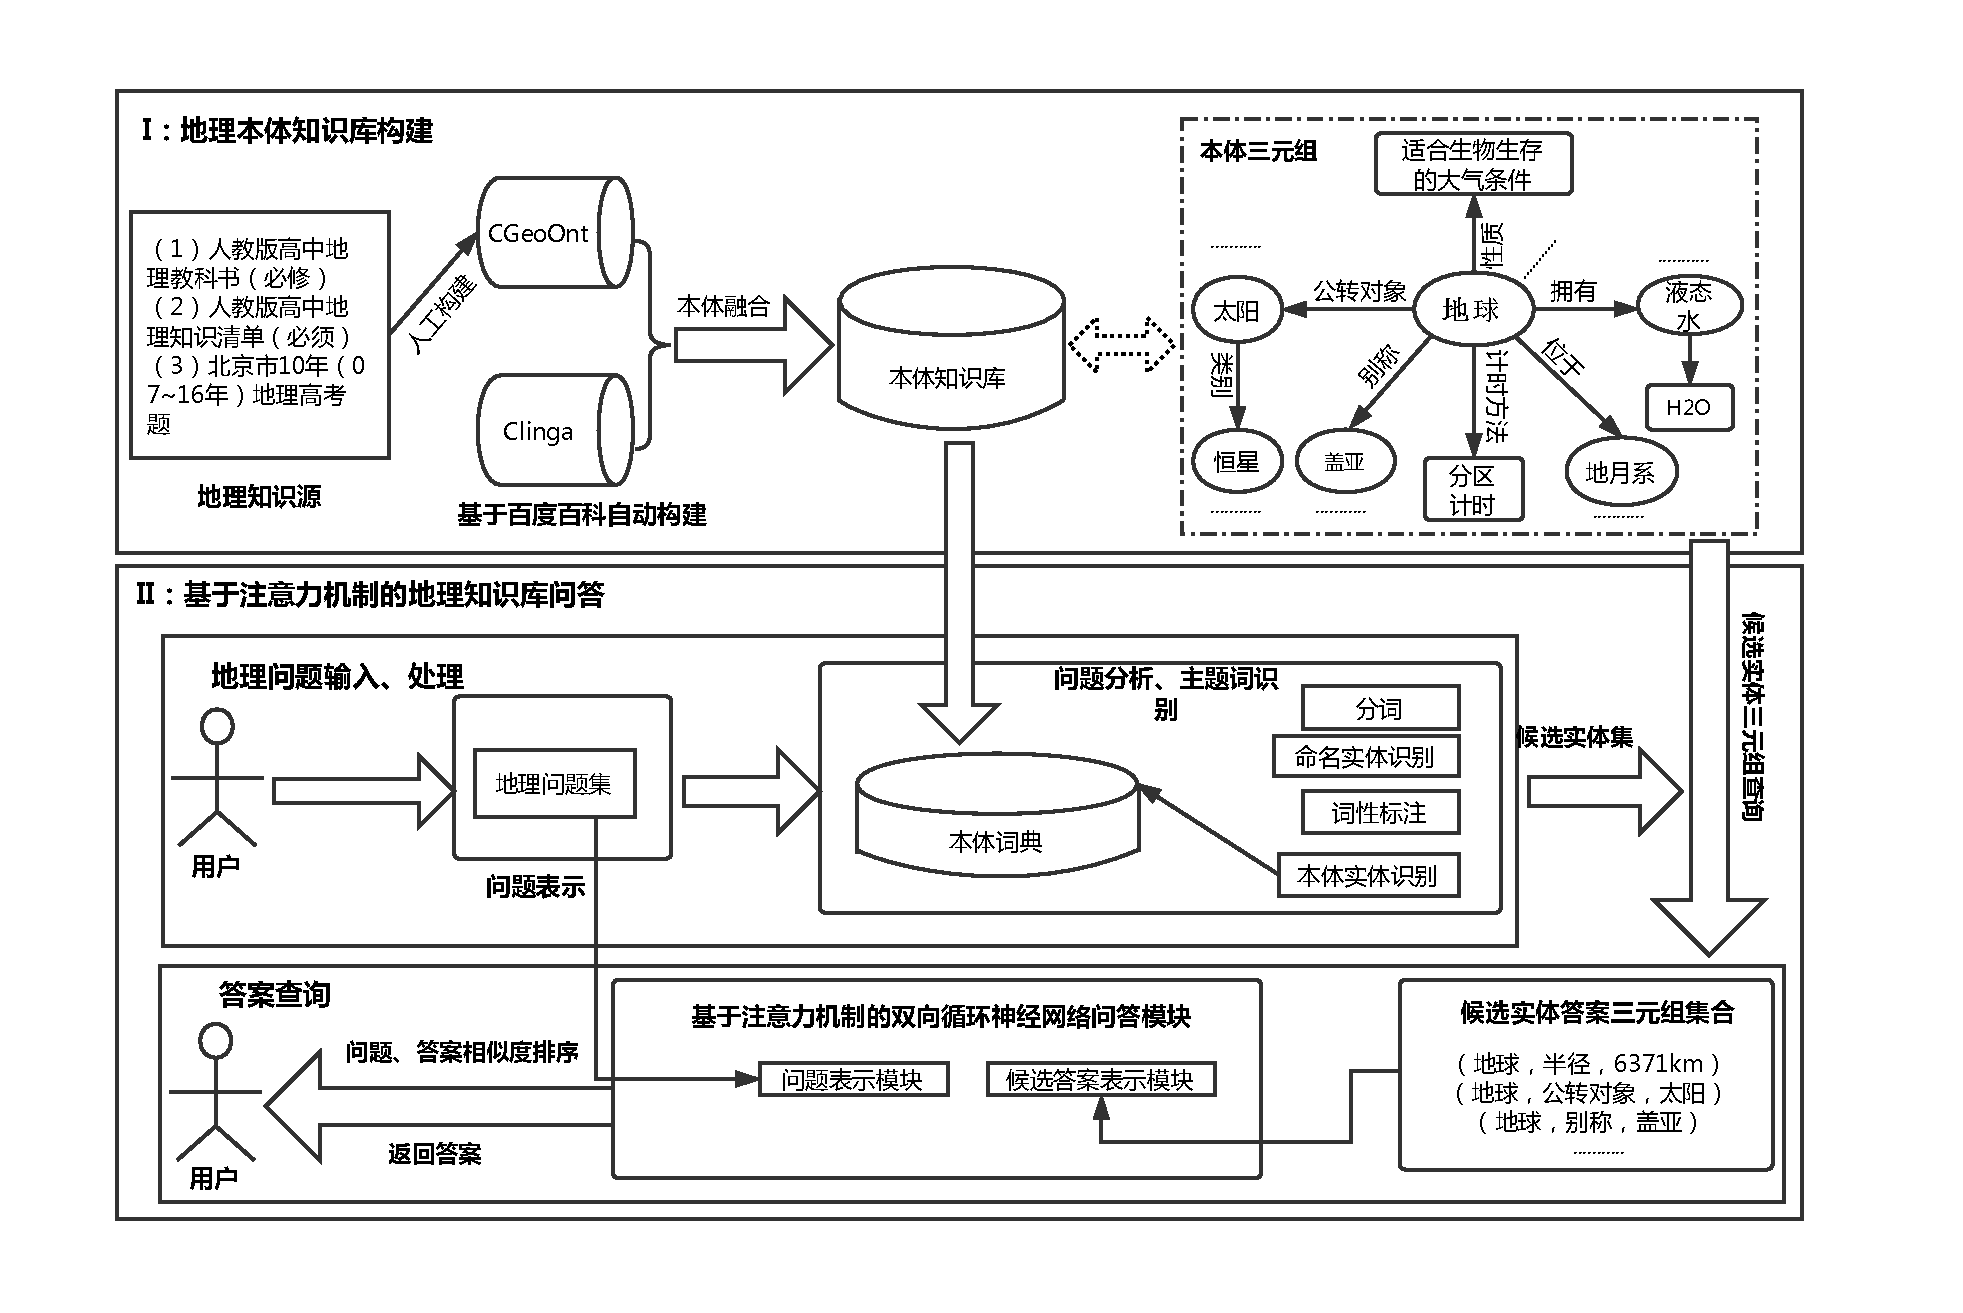
\includegraphics[height=9cm]{resource/graduation}
	\caption{基于本体的地理知识问答系统结构图}
	\label{fig:graduation}
\end{figure}

\section{地理本体知识库构建}
地理本体知识库构建内容分三个部分来介绍,先介绍地理本体CGeoOnt(chinese geographic ontology)的构建,然后介绍本体Clinga(chinese linked geographical dataset)与本体CGeoOnt融合,最后介绍本体词典生成方法。

\subsection{地理本体CGeoOnt构建}\label{section:CGeoOnt_build}
本文本体构建方法借鉴了斯坦福七步法的流程思想,但是与斯坦福的七步法有一些区别,如本文没有可以复用的本体,并且一次性列出本体的重要术语明显可操作性不强。因此,根据本文地理本体构建特点,主要分四个步骤进行构建工作,分别如下:

(1)地理知识源选取。选取本体构建所需要的资料,文档或者图形形式。

(2)地理知识体系定义。确定本体构建的三元组知识组织顺序。

(3)地理本体构建规范定义。约定本体构建的知识组织规范。

(4)地理本体基本元素定义。定义类、属性、关系,创建实例。

\subsubsection{地理知识源选取}
地理本体构建知识源来自专业的高中地理教材以及部分的高考试题。地理教材包括人教版高中地理必修一自然地理、必修二人文地理、必修三区域可持续发展、区域地理、选修三旅游地理、选修五自然灾害与防治、选修六环境保护这七本教材和一本高中地理知识清单。高中地理知识清单是专家对上述七本高中地理教材中核心考点的精确提炼以及每本书知识点的解题方法讲解。高考试题选取的是北京市近10年(2007年~2016年)的地理高考题,选取高考题作为知识源的目的是:标注人员可以根据高考题快速把握高考地理考点以及解决考点所需要的辅助知识,因此可以很有目的性的去教材中寻找需要标注的核心知识,避免标注大量对于解题无用的地理知识,大大提高了地理核心知识库构建的效率。本文地理资源均为电子资源,且格式为HTML的网页形式,里面包含文字叙述、图和表格。

\subsubsection{地理知识体系定义}
地理知识体系的定义根据《高中地理知识清单(第3次修订)》
中的组织结构进行,该高中地理知识清单包括了整个高中地理教科书中知识的组织顺序,如高中地理教材的组织先从必修地理开始,包括必修自然地理、必修人文地理、必须区域可持续发展。然后是介绍选修地理部分,包括选修旅游地理、选修自然灾害与防治和选修环境保护。对于每一本教材中的知识体系根据书中每个章节的相关主题、相关知识点和相关方法三个方面来组织,这样的好处是使知识库的知识都能够找到其知识的出处,便于后续分析知识之间的关系和知识溯源,保留知识的完整性。如在标注概念类“天体”的知识三元组时,需要标注出“天体”在书中所属的“相关主题”是“宇宙中的地球”,以及“天体”涉及的“相关知识点”是“地球的宇宙环境”和跟“天体”相关联的“相关方法”是“天体类型的判断方法”。

\subsubsection{地理本体构建规范}
地理本体构建规范主要为保证最终本体的构建形式一致,因为本体构建需要多个专业人员参与,不同人的标注主观性很大,必须经过统一的规范约束。首先,本文地理知识需要较强的表达能力且还需具备很强的推理能力,因此本文约定本体描述语言使用OWL,构建符合RDFS和OWL DL级别规范。其次,由于本文地理本体构建有很多自己的特殊定义,有些定义需要突破OWL DL的规范,因此本文构建工作不使用当前存在的本体构建工具,如protege等,本文直接以RDF三元组的语法形式Turtle\footnote{https://www.w3.org/TR/turtle/}来表示每条本体知识(三元组)。最后,本文规定个体、类、属性等的命名说明规范,统一本体的最终表现形式。

为简化三元组的表示,本文定义了本文地理本体术语的命名空间,包括自定义的三个地理本体元素——个体、属性及类的命名空间gsr、gss、gso,以及包括七个常见的本体元素命名空间:rdf、rdfs、owl、skos、xs、op和fn。以上命名空间如下所示:

% 用s表示正常的字符宽度,l代表稍微窄的字符宽度

@prefix gsr:\hphantom{sss}<http://ws.nju.edu.cn/geoscholar/resource>.

@prefix gss:\hphantom{sss}<http://ws.nju.edu.cn/geoscholar/staticOntology>.

@prefix gso:\hphantom{ssl}<http://ws.nju.edu.cn/geoscholar/ontology>.

@prefix rdf:\hphantom{sss}<http://www.w3.org/1999/02/22-rdf-syntax-ns>.

@prefix rdfs:\hphantom{ss}<http://www.w3.org/2000/01/rdf-schema>.

@prefix owl:\hphantom{ss}<http://www.w3.org/2002/07/owl>.

@prefix skos:\hphantom{ll}<http://www.w3.org/2004/02/skos/core>.

@prefix xs:\hphantom{sssl}<http://www.w3.org/2001/XMLSchema>.

@prefix op:\hphantom{ssll}<http://www.w3.org/2002/08/xquery-operators>.

@prefix fn:\hphantom{sssl}<http://www.w3.org/2005/xpath-functions>.\linebreak[3]
\\
以下为其他约定,核心思想为本体不同元素有区分度,同时见其英文名可知其中文义:
\begin{itemize}
	\item {个体:以“R\_”开头,如gsr:R\_太阳。
	}
	\item {类:以“C\_”开头,如gso:C\_天体。
	}
	\item{属性(静态属性):以“P\_”开头,两个属性owl:ObjectProperty、owl:DatatypeProperty分别以“P\_o\_”和“P\_d\_”开头。如gso:P\_o\_公转对象,gso:P\_d\_高度。
	}
	\item{个体必须声明类别owl:Class、属性必须确定是对象属性owl:ObjectProperty还是数据类型属性owl:DatatypeProperty。
	}
	\item{每个术语有且仅有一个skos:prefLabel,但是可以有多个skos:altLabel用于别名。
	}
	\item {每个术语有必要时使用skos:definition给出其定义,使用rdfs:comment对其重要方面进行评论。
	}
	\item {术语间多使用gso:relatedTo来表达它们有一定的关联性。
	}
	\item {为避免处理的复杂性,三元组中不使用空白节点( blank node )。
	}
\end{itemize}

\subsubsection{地理本体基本元素定义}
本文地理本体构建遵循自下而上的原则,按照书本知识的组织顺序构建本体,不一次性的定义其领域所有术语,而采取根据每章、每节中的考点知识构建,考点知识的确定参照10年的北京市地理高考题以及书中重点强调的考点。下面分别介绍类、属性、个体和本文特殊地理元素的具体构建。

(1)类的构建

类的构建需要声明其类型是OWL中的类,并且需要定义其唯一的名称skos:prefLabel,而且该类若有别名则需定义别名skos:altLabel,该类的父类(\text{subClassOf})若有则需要定义出。类相关的定义或者评论可以通过skos:definition和skos:comment定义出,并且若该类所对应的课文章节主题和知识点为重要考点,也应该定义出。如下举例为本文对概念类“天体”的三元组知识表示,知识三元组中的主语、谓语、宾语之间以空格表示:

gso:C\_行星\quad rdf:type\quad owl:Class\quad .

gso:C\_行星\quad skos:prefLabel\quad "行星"$^{\land\land}$xs:string\quad .

gso:C\_行星\quad rdfs:subClassOf\quad gso:C\_天体\quad .

gso:C\_行星\quad skos:definition\quad "在椭圆轨道上,环绕恒星运行、近似球状的天体,其质量比恒呈小,本身是不发光的\"$^{\land\land}$xs:string\quad .

gso:C\_行星\quad gsb:relatedToKPoint\quad gsb:M\_太阳对地球的影响\quad .

gso:C\_行星\quad gsb:relatedToKPoint\quad gsb:M\_宇宙中的地球\quad .

gso:C\_行星\quad gsb:relatedToTopic\quad gsb:M\_行星地球 .
\\

(2)属性的构建 

本文的属性包括普通的属性和本文特殊定义的属性,此节只讲述普通属性的构建,特殊定义的属性到第四节“地理特殊定义元素”介绍。本文普通属性的构建前提得明确区分对象属性owl:ObjectProperty和数据类型属性owl:DatatypeProperty,属性的性质(如对称性、传递性等)需要定义出来,便于根据属性进行相关推理。同时,对于对象属性,本文需描述属性的定义域rdfs:domain和值域rdfs:range,不好区分情形下使用总类owl:Thing描述;对于数据类型属性,数据类型的单位必须定义,如下分别为对象属性“垂直”和数据属性“宽度值”的表示:

对象属性:垂直

gso:P\_o\_垂直\quad rdf:type\quad owl:ObjectProperty\quad .(对象属性)

gso:P\_o\_垂直\quad skos:prefLabel\quad "垂直"$^{\land\land}$xs:string\quad .(属性名称)

gso:P\_o\_垂直\quad rdfs:domain\quad owl:Thing\quad .\quad (定义域为所有对象)

gso:P\_o\_垂直\quad rdfs:range\quad owl:Thing\quad .\quad (值域为所有对象)

gso:P\_o\_垂直\quad a\quad owl:SymmetricProperty\quad .\quad \quad (对称性)

gsr:R\_水平气压梯度力\quad gso:P\_o\_垂直\quad gsr:R\_等压线\quad .(属性连接的两个对象)

gso:P\_o\_垂直\quad gsb:relatedToKPoint\quad gsb:M\_大气的水平运动-风\quad .(属性涉及到的考点知识)\\

数据属性:宽度值

gso:P\_d\_宽度值\quad rdf:type\quad owl:DatatypeProperty\quad .(数据属性)

gso:P\_d\_宽度值\quad skos:prefLabel\quad "宽度值"$^{\land\land}$xs:string\quad .(属性名称)

gso:P\_d\_宽度值\quad gso:physicalQuantity\quad "宽度"$^{\land\land}$xs:string\quad .(属性单位名称)

gso:P\_d\_宽度值\quad gso:unit\quad "米"$^{\land\land}$xs:string\quad .(属性单位类型)

gso:P\_d\_宽度值\quad rdfs:domain\quad owl:Thing\quad .(定义域为所有对象)

gso:P\_d\_宽度值\quad rdfs:range\quad xs:double\quad .(值域为双精度数值)

gso:P\_d\_宽度值\quad rdfs:comment\quad "描述某物a的宽度为某个值"$^{\land\land}$xs:string\quad .(属性的一般性评论)

gsr:R\_南极附近海上最大的冰山\quad gso:P\_d\_宽度值\quad \quad "97000.0"$^{\land\land}$xs:double\quad .(属性描述的个体知识)

gso:P\_d\_宽度值\quad gsb:relatedToKPoint\quad gsb:M\_水资源与人类社会\quad .(属性相关的知识考点)

gso:P\_d\_宽度值\quad gsb:relatedToTopic\quad gsb:M\_水资源的合理利用\quad .(属性相关的知识考点章节)  \\

(3)个体的构建

个体的构建只包含标注章节中包含高考地理考点的专业术语,其它非考点术语忽略不予标注。本文个体构建遵循最重要的一个原则就是每个个体必须申明其类别,而且其类别允许为多个,这一点也符合现实世界的表示。如下为术语个体“地球”的知识表示:

gsr:R\_地球\quad skos:prefLabel\quad "地球"$^{\land\land}$xs:string\quad .\quad (个体名称)

gsr:R\_地球\quad rdf:type\quad gso:C\_行星\quad .(个体的类别,此处地球有三个标签类别)

gsr:R\_地球\quad rdf:type\quad gso:C\_物体\quad .(个体的类别)

gsr:R\_地球\quad rdf:type\quad gso:Location\quad .(个体的类别)

gsr:R\_地球\quad gso:P\_d\_性质\quad "适合生物生存的大气条件"$^{\land\land}$xs:string\quad .(个体数据-字符串属性,描述的事实是:地球拥有适合生物生存的大气条件的性质)

gsr:R\_地球\quad gso:P\_d\_轨道偏心率\quad "0"$^{\land\land}$xs:string\quad .(个体数据-字符串属性)

gsr:R\_地球\quad gso:P\_d\_计时方法\quad "分区计时"$^{\land\land}$xs:string\quad .(个体数据-字符串属性)

gsr:R\_地球\quad gso:P\_d\_时区数量\quad "24"$^{\land\land}$xs:integer\quad .(个体数据-整型属性)

gsr:R\_地球\quad gso:P\_d\_平均密度\quad "5"$^{\land\land}$xs:string\quad .(个体数据-字符串属性)

gsr:R\_地球\quad gso:P\_o\_公转对象\quad gsr:R\_太阳\quad .(个体的对象属性)

gsr:R\_地球\quad gso:P\_o\_天然卫星\quad gsr:R\_月球\quad .(个体的对象属性)

gsr:R\_地球\quad gso:P\_o\_拥有\quad gsr:R\_液态水\quad .(个体的对象属性)

gsr:R\_地球\quad gso:P\_o\_南部\quad gsr:R\_南半球\quad .(个体的对象属性)
\\

(4)地理本体特色元素

$\P$静态属性
		
静态属性,本文前缀表示为gss,是为增强地理知识的表达能力而设定的,需与普通属性gso相区别。静态属性严格上并不满足OWL的属性规范,因为OWL的属性连接的可以是两个个体或者一个个体一个数据类型数据,而本文的静态属性描述的是类的属性特征。静态属性重要的特性是静态属性所描述的类所包含的所有个体均具有该静态属性特征,这一点类似于个体继承类的特征。由于静态属性是对一类个体的描述,本文可以允许其不申明定义域rdfs:domain和值域rdfs:range,但是该静态属性仍然区分是对象属性owl:ObjectProperty还是数据类型属性owl:DatatypeProperty,如下对类“暖流”定义了一个静态属性“作用”。

gss:P\_d\_作用\quad rdf:type \quad owl:DatatypeProperty\quad .(gss申明静态数据类型属性)

gso:C\_暖流\quad gss:P\_d\_作用\quad "对沿岸气候增温增湿"$^{\land\land}$xs:string\quad .

gsr:R\_北大西洋暖流\quad rdf:type\quad gso:C\_暖流.(申明暖流的个体-北大西洋暖流)
\\
则表明:北大西洋暖流同样具有暖流的静态属性特性,也即:

gsr:R\_北大西洋暖流\quad gso:P\_d\_作用\quad "对沿岸气候增温增湿"$^{\land\land}$xs:string\quad .
	\\
	
$\P$封闭集

封闭集用符号gso:isClosed表示,包括类和属性的封闭集。类的封闭集表示某个类的实例可以全部列举出,属性的封闭集表示某个个体在该属性上取值是封闭的,即包含有限的取值且可以穷举出来。

	$\bullet$类封闭集知识举例:地球的极点包括南极点、北极点

gsr:R\_北极点\quad a\quad gso:C\_地球极点\quad .

gsr:R\_南极点\quad a\quad gso:C\_地球极点\quad .

gso:C\_地球极点\quad gso:isClosed\quad "true"$^{\land\land}$xs:boolean\quad .

地球极点类在封闭集gso:isClosed属性上取值为true,说明地球极点的取值实例个体已经完整了,只有南极点和北极点。

$\bullet$属性封闭集知识举例:太阳大气层由里到外可分为光球、色球、日冕三层。

gsr:R\_太阳大气层\quad gso:P\_o\_包含\quad gsr:R\_光球\quad ;

gsr:R\_太阳大气层\quad gso:P\_o\_包含\quad gsr:R\_色球\quad ;

gsr:R\_太阳大气层\quad gso:P\_o\_包含\quad gsr:R\_日冕\quad .

gso:P\_o\_包含\quad gso:isClosedAt\quad gsr:R\_太阳大气层\quad.

该知识表示“包含”属性在个体“太阳大气层”上处于封闭状态,说明太阳大气层只包括光球、色球和日冕三层。
	\\

$\P$地理数值类型

常见的数值类型属性的取值都较为明确,如使用整型xs:integer,双精度浮点型xs:double来表示。然而,在地理学科中,大多数出现的数值都不是精确值,往往是某种程度上的近似值。下面介绍本文几种类型的近似值处理介绍:

$\bullet$约取值

约取值的主要描述特征为“某某约为多少”,此种情况本文视作精确值处理,如知识:太阳表面的温度大约为6000K,直接取6000K作为温度数值,表示如下:

gsr:R\_太阳\quad gso:P\_d\_表面温度\quad "6000"$^{\land\land}$xs:decimal .
\\

$\bullet$表示“几”

对于地理知识源中包含“几”的数值描述,本文使用两种方法进行标注,第一种是查阅相关的权威资料,了解其具体的值;第二种是在无法通过其它辅助资料查询到相关精确数值时,使用1~9加上单位的范围值表示。如下两种举例:

地理知识:色球厚度约为几千千米,实际上通过查阅维基百科可以发现,“色球厚度大约是2,000公里”,因此可以表示如下:

gsr:R\_色球\quad gso:P\_d\_厚度\quad “2e6”$^{\land\land}$xs:double\quad .

如果无法查阅其他资料得到准确值,则采取范围区间值来表示,如下:

gsr:R\_色球\quad gso:P\_d\_厚度\quad "(1e6, 9e6)"$^{\land\land}$\quad xs:impreciseInterval\quad .
\\

$\bullet$范围值

本文标注过程中主要遇到三种范围值的表述,第一种为取值唯一,但不精确,第二种为条件缺省时导致的取值不确定,第三种为无法精确到确定的取值区间。

第一种范围值使用不精确的区间值xs:impreciseInterval表示,以圆周率举例,圆周率的值为3.1415926~3.1415927范围之间。或者再如地理知识:崇明岛全岛的面积为1200多平方千米,可以表示如下:

gsr:R\_崇明岛\quad gso:P\_d\_面积值\quad "(1.201e9, 1.299e9)"$^{\land\land}$xs:impreciseInterval\quad .

第二种范围值使用不明确的区间值xs:unclearInterval表示,如日地距离的取值,(时间不同时,日地距离亦不同),某省某刻的温度(具体的地点不同时,温度也不同)。这样的例子当补充了具体的条件,如具体时间、具体地点后就有可能转换为精确值。本文把此种复杂的条件限制使用最低到最高的区间值来表示,如下表示地球大气上界的高度不同时间的范围值:

gsr:R\_地球大气上界\quad gso:P\_d\_高度\quad "(2e6,  3e6)"$^{\land\land}$xs:unclearInterval\quad .

第三种使用不能被精确为确定值的区间xs:scopeInterval表示,如没有最大值的开区间,以地理知识为例:亚热带季风气候年降水量在800mm以上,范围值只有下界值,没有上界值,因此此种形式本文使用开区间表示,如下:


gsr:R\_亚热带季风气候\quad gso:P\_d\_年降水量\quad "[0.8, )"$^{\land\land}$xs:scopeInterval\quad .
\\

$\bullet$地理区域表示

地理区域主要指存在于空间中且可以准确定位的空间位置。地理中常常考察地理地点之间的位置关系(接壤、方向、包含等),因此对于地理重要地点的位置表示,需要准确细致的刻画。本文将空间所有事物定义为一个大类,记作gso:SpatialThing,将可以空间定位的地点定义为空间事物类的子类,记作gso:Location。如下先介绍空间位置关系,后介绍利用空间关系来表示空间位置。

空间关系:

空间关系用于描述两个可定位地点位置的相对方位关系,从某种程度上来看它也是一种对象属性,表达两个空间位置的关系。本文定义的位置关系都符合地理领域的方位表达方式,本文以常见的方位关系“位于”、“中部”来说明。“位于”表示一个位置在另一个位置上,属于一直包含的关系。“中部”表示对一个位置的方向约束,如中国中部等。如下为具体的地理知识表示:“基拉韦厄火山位于北太平洋中部的夏威夷群岛上”,本文需要准确表示出“位于”关系,北太平洋中部和被太平洋的方位“中部”关系

gsr:R\_基拉韦厄火山\quad rdf:type\quad  gso:Location\quad  .

gsr:R\_夏威夷群岛\quad rdf:type\quad  gso:Location\quad  .

gsr:R\_北太平洋\quad rdf:type\quad  gso:Location\quad  .

gsr:R\_北太平洋中部\quad rdf:type\quad  gso:SpatialThing\quad  .

gsr:R\_基拉韦厄火山\quad  gso:P\_o\_位于\quad  gsr:R\_夏威夷群岛\quad  .

gsr:R\_夏威夷群岛\quad  gso:P\_o\_位于\quad  gsr:R\_北太平洋中部\quad  .

gsr:R\_北太平洋\quad  gso:P\_o\_中部\quad  gsr:R\_北太平洋中部\quad  .
\\

空间位置:

对于空间位置,尤其是需要通过复杂空间关系来表示的空间位置,先得将其声明为gso:SpatialThing的实例,然后通过空间关系属性(谓词),建立与其他空间位置的关系,最后通过与其它位置构成的关系来整体表示该空间位置。如地理知识:“亚热带季风气候分布地区为我国秦岭-淮河以南、朝鲜半岛南部、日本群岛南部”,该知识中包含的“秦岭-淮河以南”、“朝鲜半岛南部”和“日本群岛南部”这三个带有方向限定的位置,需以本文定义的空间关系“南方”、“南部”并结合具体位置来联合表示,比如“秦岭-淮河以南”需要定义为“秦岭-淮河”的空间关系“南方”,具体表示如下:

gsr:R\_秦岭-淮河\quad rdf:type\quad gso:Location\quad .

gsr:R\_日本群岛\quad rdf:type\quad gso:Location\quad .

gsr:R\_朝鲜半岛\quad rdf:type\quad gso:Location\quad .

gsr:R\_秦岭-淮河以南\quad rdf:type\quad gso:SpatialThing\quad .

gsr:R\_日本群岛南部\quad rdf:type\quad gso:SpatialThing\quad .

gsr:R\_朝鲜半岛南部\quad rdf:type\quad gso:SpatialThing\quad .

gsr:R\_秦岭-淮河\quad gso:P\_o\_南方\quad gsr:R\_秦岭-淮河以南\quad .

gsr:R\_日本群岛\quad gso:P\_o\_南部\quad gsr:R\_日本群岛南部\quad .

gsr:R\_朝鲜半岛\quad gso:P\_o\_南部\quad gsr:R\_朝鲜半岛南部\quad .

gsr:R\_亚热带季风气候\quad gso:P\_o\_分布地区\quad gsr:R\_秦岭-淮河以南\quad ,\quad 

gsr:R\_亚热带季风气候\quad gso:P\_o\_分布地区\quad gsr:R\_日本群岛南部\quad ,\quad 

gsr:R\_亚热带季风气候\quad gso:P\_o\_分布地区\quad gsr:R\_朝鲜半岛南部\quad .
\\
再如“接壤”位置之间的表示,如知识:“亚欧板块和太平洋板块的交界处地震多发
”,需要表现“亚欧板块”与“太平洋板块”的"相接"也即“接壤”关系。

gsr:R\_亚欧板块\quad rdf:type \quad gso:Location\quad .

gsr:R\_太平洋板块\quad rdf:type \quad gso:Location\quad .

gsr:R\_亚欧板块\quad gso:P\_o\_相接\quad gsr:R\_太平洋板块\quad .

gsr:R\_亚欧板块和太平洋板块的交界处\quad rdf:type \quad gso:SpatialThing\quad ;\quad 

gsr:R\_亚欧板块和太平洋板块交界处\quad gso:P\_o\_相接\quad gsr:R\_亚欧板块\quad ;

gsr:R\_亚欧板块和太平洋板块交界处\quad gso:P\_o\_相接\quad gsr:R\_太平洋板块\quad ;

gsr:R\_亚欧板块和太平洋板块交界处\quad gso:P\_d\_地震发生率\quad "多"^^xs:string .
\\

$\bullet$过程表示

本文过程是指地理中一些现象在一系列条件下通过一系列步骤而形成的总称,常常有顺序过程和循环过程。本文将过程定义为一个大类gso:Process,然后顺序过程gso:SequentialProcess和循环过程CircularProcess分别申明为其子类。对于顺序过程或者循环过程,都需要严格的定义其形成所需要的步骤,以及每个步骤上面的步骤条件。具体定义如下:\\
先申明类:

gso:Process\quad rdf:type\quad owl:Class\quad .\quad (过程类)

gso:CircularProcess\quad rdfs:subClassOf\quad gso:Process\quad .(循环型过程类)

gso:SequentialProcess\quad rdfs:subClassOf\quad gso:Process\quad .\quad (顺序型过程类)

gso:StepOfProcess\quad rdf:type\quad owl:Class\quad .(过程的步骤类)
\\
再申明条件、步骤属性:

gso:condition4Step\quad rdf:type\quad owl:DatatypeProperty\quad .\quad (步骤条件,值为字符串)

gso:condition4Step\quad rdfs:domain\quad gso:StepOfProcess\quad .

gso:stepDesc\quad rdf:type\quad owl:DatatypeProperty\quad .\quad (步骤文字描述,取值为字符串)

gso:stepDesc\quad rdfs:domain\quad gso:StepOfProcess\quad .

gso:stepNum\quad rdf:type\quad owl:DatatypeProperty\quad .\quad (步骤的序号,第几个步骤,取值为正整数)

gso:stepNum\quad rdfs:domain\quad gso:StepOfProcess .

如下复杂地理过程知识的具体表示:“冷锋过境前,会受单一暖气团的控制,温暖晴朗。当冷气团主动移动向暖气团时,较重的冷气团会插入暖气团下面,使暖气团被迫的抬升。暖气团在抬升的过程中逐渐的冷却,其中水汽易凝结成云。如果暖空气中含有大量水汽,那么可能会导致雨雪天气。冷锋移动速度较快,常常带来较强的风。冷锋过境后,冷气团替代原来暖气团的位置,气压升高,气温降低,湿度骤降,天气则转好。”

上述叙述的是地理现象“冷锋过境”的形成过程,如下具体表示:\\
先申明“过程”和“步骤”:

gsr:R\_冷锋过境过程\quad rdf:type\quad \quad gso:SequentialProcess\quad .

gsr:R\_冷锋过境过程\quad gso:numberOfSteps\quad "3"$^{\land\land}$xs:positiveInteger\quad .

gsr:R\_冷锋过境步骤\_1\quad rdf:type\quad \quad gso:StepOfProcess\quad .

gsr:R\_冷锋过境步骤\_2\quad rdf:type\quad \quad gso:StepOfProcess\quad .

gsr:R\_冷锋过境步骤\_3\quad rdf:type\quad \quad gso:StepOfProcess\quad .

gsr:R\_冷锋过境过程\quad gso:includesStep\quad gsr:R\_冷锋过境步骤\_1\quad ,\quad 

gsr:R\_冷锋过境过程\quad gso:includesStep\quad gsr:R\_冷锋过境步骤\_2\quad ,\quad 

gsr:R\_冷锋过境过程\quad gso:includesStep\quad gsr:R\_冷锋过境步骤\_3\quad .
\\
再申明“步骤”的文字描述gso:stepDesc和条件gso:condition4Step:

gsr:R\_冷锋过境步骤\_1\quad gso:stepNum\quad "1"$^{\land\land}$xs:positiveInteger\quad ;

gso:stepDesc\quad "当冷气团主动移向暖气团时,较重的冷气团插入暖气团下面,使暖气团被迫抬升。"$^{\land\land}$xs:string\quad .

gsr:R\_冷锋过境步骤\_2\quad gso:stepNum\quad "2"$^{\land\land}$xs:positiveInteger\quad ;

gsr:R\_冷锋过境步骤\_2\quad gso:stepDesc\quad "暖气团在抬升过程中逐渐冷却,其中水汽容易凝结成云。"$^{\land\land}$xs:string\quad .

gsr:R\_冷锋过境步骤\_3\quad gso:stepNum\quad "3"$^{\land\land}$xs:positiveInteger\quad ;

gsr:R\_冷锋过境步骤\_3\quad gso:condition4Step\quad "暖空气中含有大量水汽。"$^{\land\land}$xs:string\quad ;

gsr:R\_冷锋过境步骤\_3\quad gso:stepDesc\quad "如果暖空气中含有大量的水汽,那么可能会带来雨雪天气。"$^{\land\land}$xs:string\quad .

此“冷锋过境”过程中实际上也包含了不同时段的“天气变化”,因此“冷锋过境中的天气变化”也需要表示为一个顺序过程,这样在考察“冷锋过境”与天气变化的关系是,可以运用此结构化的知识表示。具体表示如下:
\\
申明“冷锋过境中的天气变化”为顺序过程:

gsr:R\_冷锋过境中的天气变化\quad rdf:type \quad gso:SequentialProcess\quad ;

gsr:R\_冷锋过境中的天气变化\quad gso:numberOfSteps\quad "3"$^{\land\land}$xs:positiveInteger\quad .

gsr:R\_冷锋过境中天气变化的步骤\_1\quad rdf:type \quad gso:StepOfProcess\quad .

gsr:R\_冷锋过境中天气变化的步骤\_2\quad rdf:type \quad gso:StepOfProcess\quad .

gsr:R\_冷锋过境中天气变化的步骤\_3\quad rdf:type \quad gso:StepOfProcess\quad .

gsr:R\_冷锋过境过程中的天气变化\quad gso:includesStep\quad gsr:R\_冷锋过境中天气变化的步骤\_1\quad ,\quad 

gsr:R\_冷锋过境过程中的天气变化\quad gso:includesStep\quad gsr:R\_冷锋过境中天气变化的步骤\_2\quad ,\quad 

gsr:R\_冷锋过境过程中的天气变化\quad gso:includesStep\quad gsr:R\_冷锋过境中天气变化的步骤\_3\quad .
\\
申明“冷锋过境中的天气变化”的每个步骤的内容和条件:

gsr:R\_冷锋过境中天气变化的步骤\_1\quad gso:stepNum\quad "1"$^{\land\land}$xs:positiveInteger\quad ;

gsr:R\_冷锋过境中天气变化的步骤\_1\quad gso:condition4Step\quad "过境前"$^{\land\land}$xs:string\quad ;

gsr:R\_冷锋过境中天气变化的步骤\_1\quad gso:stepDesc\quad "过境前,单一暖气团控制,温暖晴朗。"$^{\land\land}$xs:string\quad .

gsr:R\_冷锋过境中天气变化的步骤\_2\quad gso:stepNum\quad "2"$^{\land\land}$xs:positiveInteger\quad ;

gsr:R\_冷锋过境中天气变化的步骤\_2\quad gso:condition4Step\quad "过境时"$^{\land\land}$xs:string\quad ;

gsr:R\_冷锋过境中天气变化的步骤\_2\quad gso:stepDesc\quad "过境时,常有阴天、下雨、刮风、降温等天气现象。"$^{\land\land}$xs:string\quad .

gsr:R\_冷锋过境中天气变化的步骤\_3\quad gso:stepNum\quad "3"$^{\land\land}$xs:positiveInteger\quad ;

gsr:R\_冷锋过境中天气变化的步骤\_3\quad gso:condition4Step\quad "过境后"$^{\land\land}$xs:string\quad ;

gsr:R\_冷锋过境中天气变化的步骤\_3\quad gso:stepDesc\quad "过境后,气强和湿度骤降,天气转睛。"$^{\land\land}$xs:string\quad .

\subsection{地理本体融合}
本文地理核心知识库由构建的两个本体融合而成。这两个本体分别是本文手工构建的CGeoOnt和863项目组基于百度百科自动构建的本体Clinga。本节先介绍Clinga的相关情况,后介绍两个地理本体的融合方法。

\subsubsection{本体Clinga}

本体Clinga\footnote{http://ws.nju.edu.cn/clinga/}为863项目组Hu【26】等人根据百度百科自动抽取构建的中文地理链接数据集(Chinese linked geographical dataset)。Clinga的本体Schema为Hu等人人工根据地理领域特点来定义,他们将地理分为自然地理和人文地理两个大类,然后在这两个大类下再依次细分为多个小类,最后形成Clinga的schema,具体如摘要图\ref{fig:clinga}所示。通过定义好的本体schema对自动抽取到的百度百科概念做分类,只选取满足定义好的本体schema类别的实体,最后对每个百科概念页面结构化成三元组形式,最终得到包含624,391个实体概念、130个类别、73,326,425个三元组的本体。Clinga中知识的组织形式为主、谓、宾,即( s, p, o)三元组。例如( A6906464, 公转对象,A6768329)表示“地球绕着太阳公转”, A6906464和 A6768329 分别对应地球、太阳在知识库中的存储ID,“公转对象”表示地球和太阳的一种属性关系。

\begin{figure}[!htb]
	\centering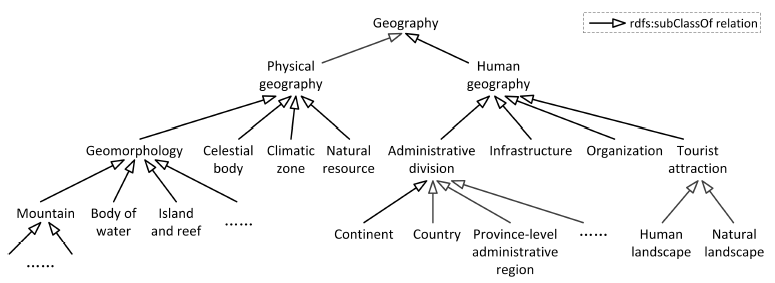
\includegraphics[height=5cm]{resource/clinga}
	\caption{Clinga本体层次结构定义摘要}
	\label{fig:clinga}
\end{figure}

图\ref{fig:clinga}仅仅为Clinga本体结构的一个摘要,有向图的跟节点为总大类地理,然后箭头被指向的是其两个子类自然地理和人文地理,然后依次为这两个子类的定义,依次类推,实际图中的类共有130个,其中的35个叶子类为GeoNames\footnote{http://www.geonames.org/}中没有的类,更具体的情况请参加Hu等人的工作。

\subsubsection{地理本体融合方法}
Clinga 与 CGeoOnt 的 Schema 定义存在一定差异,本文需要将这两个本体进行融合得到一个更综合的地理知识库。本文构建的CGeoOnt 包含类和属性3,000 余个,相关 RDF 三元组 25,000 余条,概念类的定义粒度相比Clinga来说比较细。由于CGeoOnt 本体相对量较小,本文采取将本体CGeoOnt的Schema映射到Clinga的Schema上,具体操作流程如下:

( 1) Clinga 中实体只保留其在百度百科 infobox 域中信息三元组,去掉其 section 文本三元组。

( 2) 运用启发式规则,根据 CGeoOnt 中实体的名称将其类别映射到 Clinga 中的类别。如, CGeoOnt中“黄山”会被映射到 Clinga 中的类 “山”。

( 3) 人工校验( 2) 中映射结果。

( 4)得到最终本体知识库三元组 4,850,435 条。

\subsection{地理本体词典生成}
本文需要根据构建的地理知识库生成地理概念词典,这些概念包含知识库中的实体和类及两者的同义词。生成的地理本体词典主要用于判断某个命名实体是否属于本文地理知识库的范畴,以便提供相关候选实体的知识库信息,同时也为了查询同一个实体的不同别名。

地理本体词典的生成主要工作为抽取地理概念的同义词,由于本文的知识库有两部分数据来源,分别是本体Clinga和本体CGeoOnt。Clinga中的概念抽取自百度百科,因此可以通过规则模板来抽取某个概念的同义词,本文统计发现属性名为中文名、英文名、外文名、原名、别名、中文名称、其他名称、别称和又叫的均可以当作概念的同义词。由于百科知识组织的主观性强,有的实体在表示时后面常常跟有括号,如“地球 别名 盖亚(Gaia)”,针对此种情况需要将别名值中带有括号的部分也抽取出来,并作为该概念的同义词,如此处的Gaia也作为地球的同义词。CGeoOnt中的同义词已经被标注人员标注出,只需要抽取概念的skos:altLabel属性就可以找出该概念的同义词。通过上述,方法,本文得到共包含75,1103个概念同义词词典。

\section{基于注意力机制的地理知识库问答}
基于注意力机制的中文地理知识库问答指根据本文构建的中文地理知识库,运用基于注意力机制的双向循环神经网络问答模型,对用户提出的地理问题,从知识库搜索出问题答案三元组的总过程。该系统问答流程如图\ref{fig:qa_overview},图\ref{fig:qa_overview}表示的是地理问题“2016年北京处暑节气是什么时间”被回答的流程。首先任务是识别该地理问题中的主题实体,也就是问题是围绕哪个实体概念在提问的,如此问题中考察的是“北京的处暑节气时间”,是考察跟“北京”相关的事实性知识,因此“北京”为主题实体。然后,根据主题实体“北京”从本文构建的知识库中查询出与“北京”直接相连的所有实体作为候选实体,此处为首尔和华盛顿。最后使用双向循环神经网络对此问题和候选答案三元组-北京、首尔、华盛顿的三元组进行词向量表示,取问题与候选答案三元组相似度最大的作为该问题的答案。

总结本文知识库问答任务分为如下四步进行:

\begin{figure}[!htb]
	\centering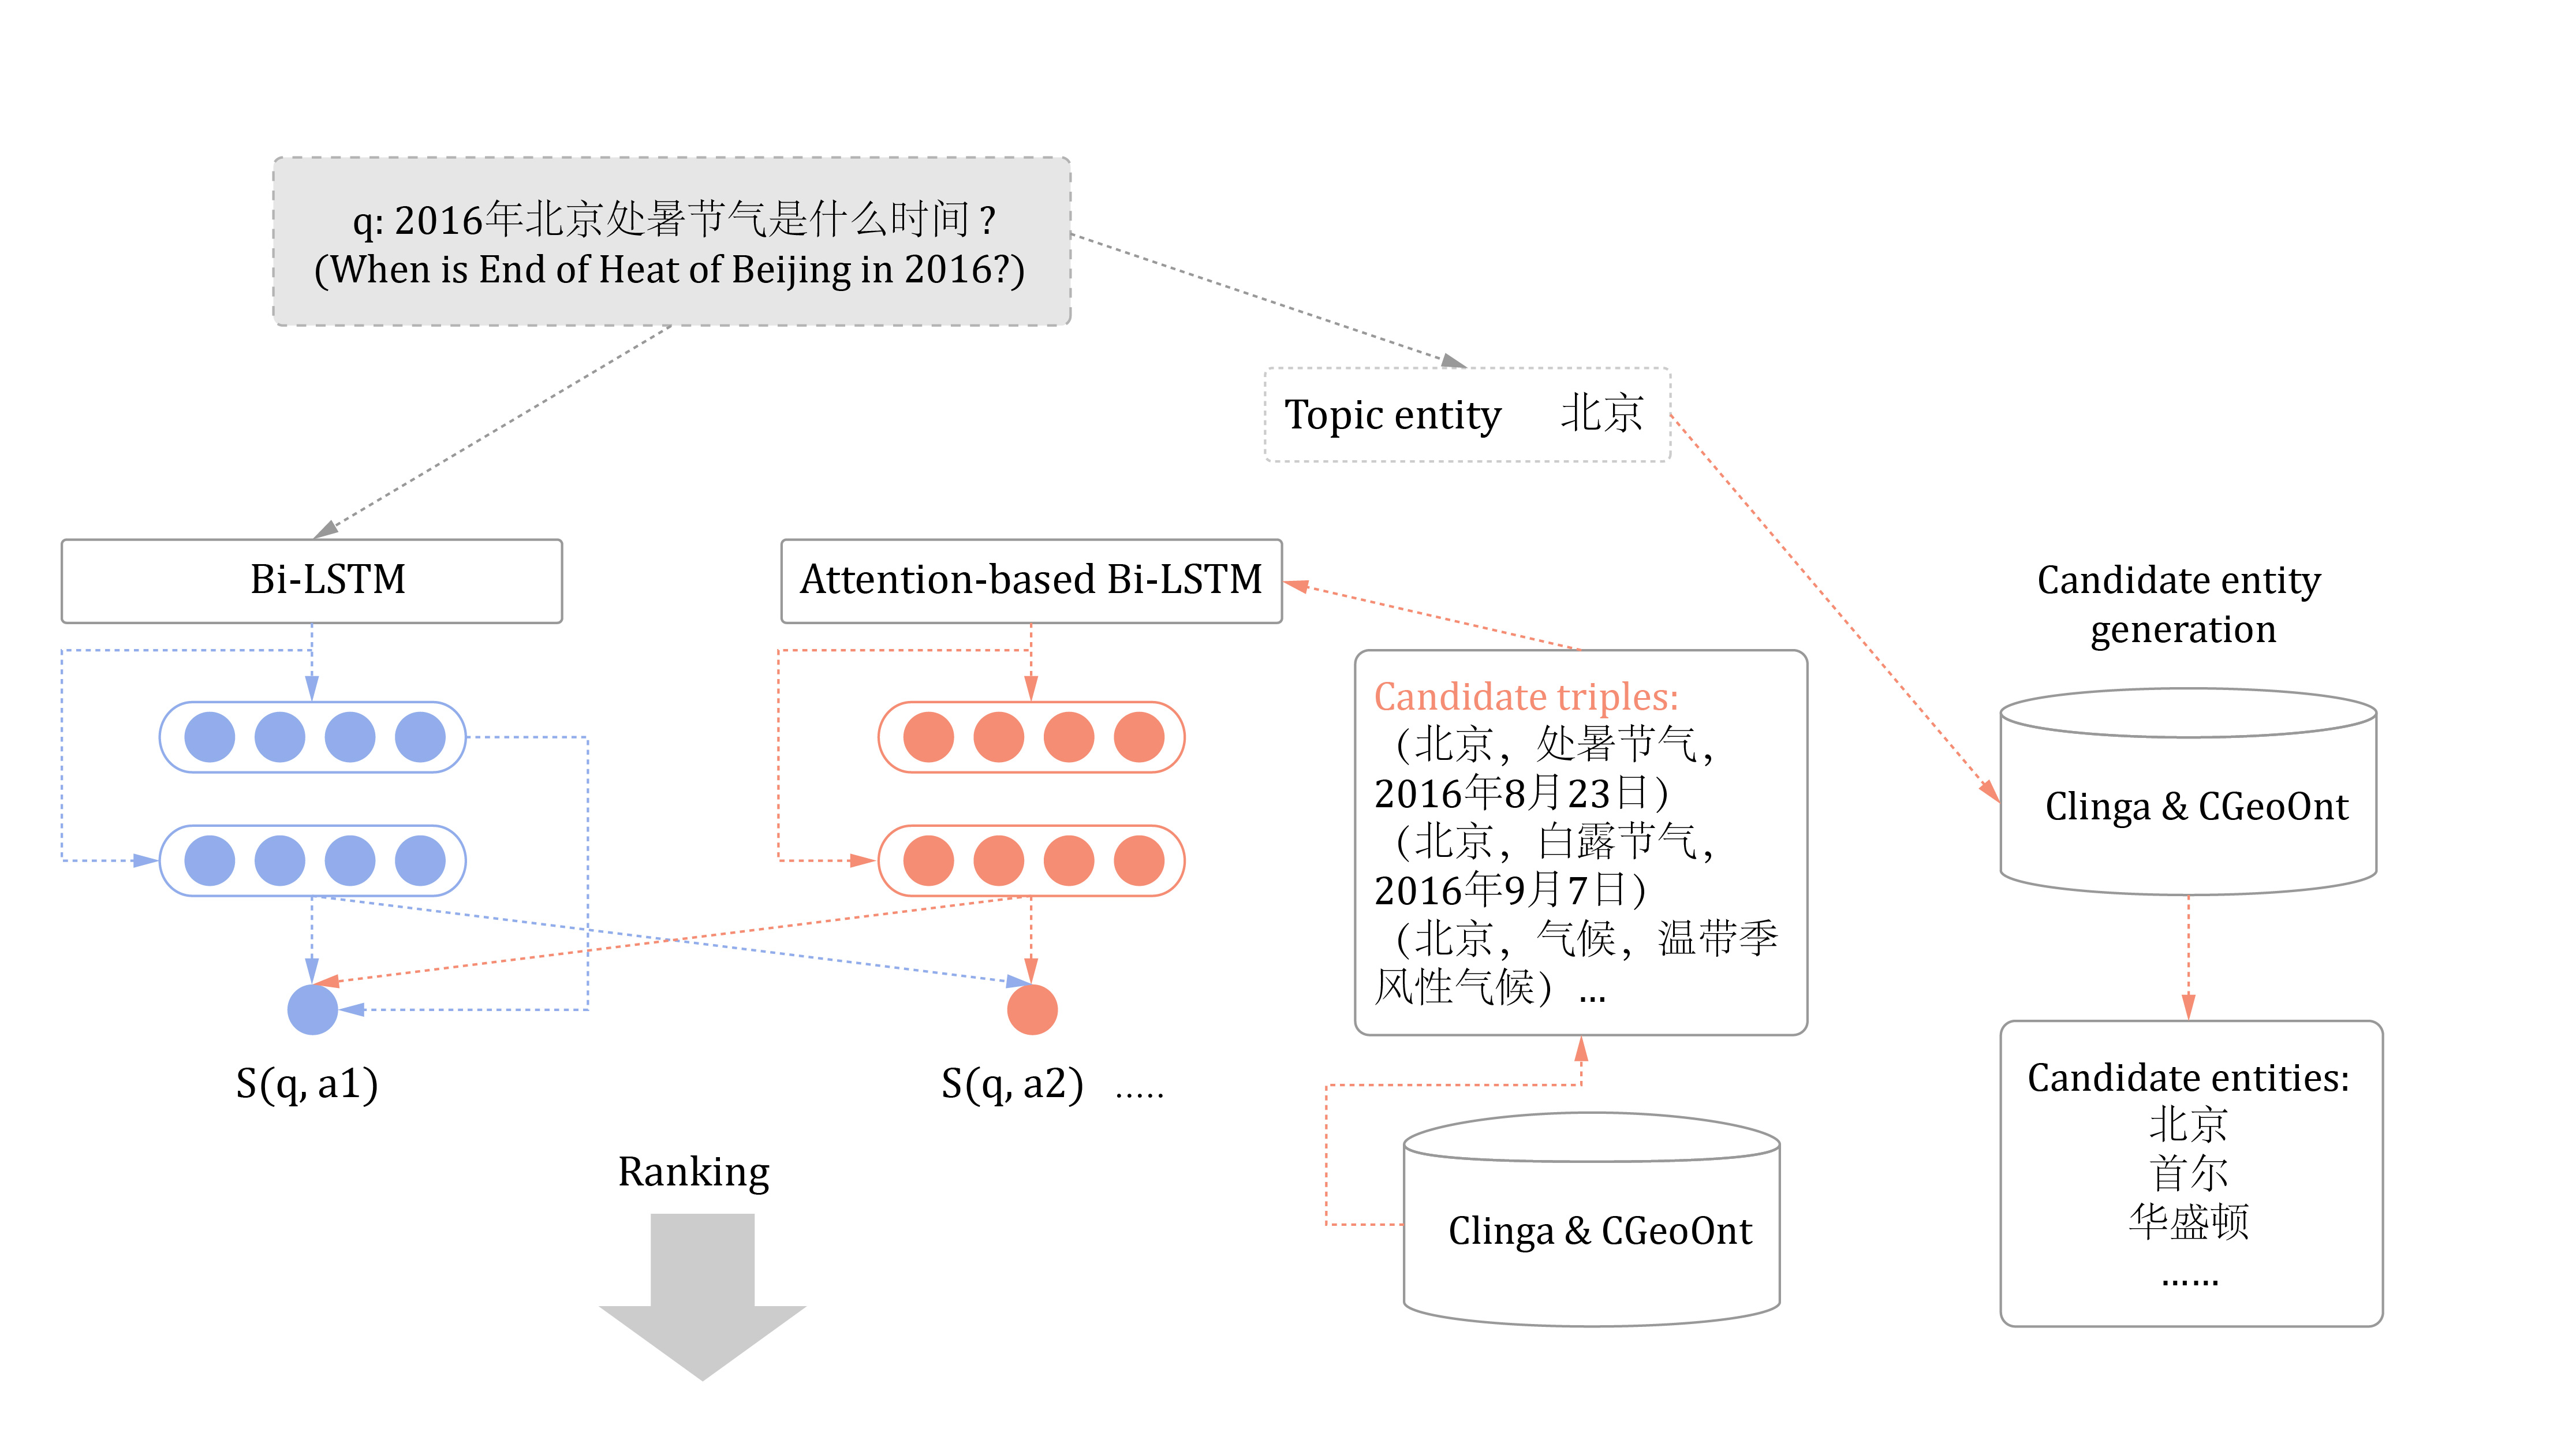
\includegraphics[height=7cm]{resource/qa_overview}
	\caption{基于注意力机制的地理知识库问答流程}
	\label{fig:qa_overview}
\end{figure}

( 1)识别地理问题中涉及的主题实体,根据主题实体生成候选实体集。

(2)根据候选实体集查询知识库,返回候选实体三元组。

( 3)使用双向 LSTM 神经网络编码问题(问题词序列表示成词向量),使用基于注意力机制的双向 LSTM编码候选答案三元组。

( 4)计算问题与每个候选答案三元组的余弦相似度值,返回余弦值最大的三元组作为最终答案(有时返回多个最终答案, 详见 3.4)。

\subsection{地理知识库问答实现方法}
此部分首先介绍候选答案实体三元组的生成方法,然后介绍本文表示问题、答案的基本模型 LSTM,再到其变种双向 LSTM 和结合注意力机制的双向LSTM 模型,最后介绍模型的训练方法和问答最终答案的选择策略。

\subsubsection{候选答案实体三元组生成}
生成候选实体三元组需要识别问题中的主题实体,主题实体也应当存在于本文所使用的知识库中,如果知识库中不存在此主题实体,则问题回答失败。

本文根据知识库构建实体概念词典以及实体概念别名词典,确定知识库能够回答的实体问题范围。候选答案实体三元组生成的关键是识别出问题中的主题实体,如下(1)-—)主题实体识别流程,(4)-(5)步为根据主题实体生成候选答案实体三元组:

(1)使用分词工具jieba\footnote{https://pypi.org/project/jieba/}将问题进行分词,生成句子的词序列。

(2)对词序列进行命名实体识别(Named Entity Recognition, NER)、词性标注(Part  of  Speech, POS), 识别其中的命名实体、名词以及名词词组,本文成为候选主题实体集。

(3)遍历(2)步中生成的候选主题实体集,查询该候选实体是否在本文本体词典中,若存在,则该实体视作主题实体;若为本体词典中词的字串(不包含相等的情况),亦将该实体视作主题实体;若所有候选主题实体都不存在于本体词典中,则本问题没有主题实体,此题目超出本文知识库的回答范围。

(4)从本文地理知识库中获取跟主题实体一跳1-hop\footnote{1-hop表示跟实体距离为1的实体,距离即相连的关系边}和二跳2-hop的实体集合作为候选答案实体集。

(5)最后,从知识库查询出候选答案实体集每个实体的三元组信息,构成目标候选答案实体三元组集合。


\subsubsection{3.1.2\quad 地理问题、候选答案表示}
本节讲述如何将地理问题和候选答案这样的文本序列表示成词向量(word embedding)形式。本文表示地理和候选答案的基础模型为循环神经网络( Recurrent Neural Networks,RNN),本节介绍使用RNN的变种LSTM模型来表示地理问题和答案,本文先介绍RNN表示序列数据的原理,后依次介绍使用基于基本的LSTM表示问题、答案,基于Bi-LSTM来表示问题答案和基于Attention的Bi-LSTM表示答案。
\\

$\P$ RNN表示序列数据原理

RNN的网络结构如图\ref{fig:rnn_structure}所示,图的左边部分表示RNN的循环结构图,RNN的主体结构单元A处理来自当前时刻的输入$x_{i}$和上一时刻A输出的隐含状态。图的右边是左边图的展开形式。RNN中每一层不仅输出$h_{i}$到下一层,而且同时还输出一个隐含状态(hidden state),该隐含状态表示到当前层到前面所有层的保存信息,可以形象化地理解为当前到之前层的所有信息的综合记忆,下一层可以利用上一层输出的隐含状态信息。因此,RNN的这种网络特征结构也使得其非常时候处理前后有依赖关系的数据序列。

\begin{figure}[!htb]
	\centering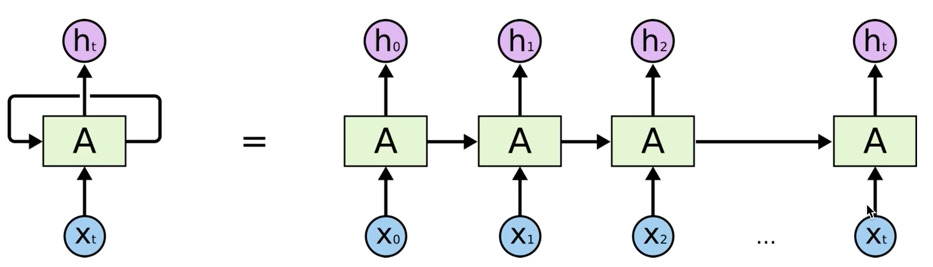
\includegraphics[height=3cm]{resource/rnn_structure}
	\caption{RNN网络结构}
	\label{fig:rnn_structure}
\end{figure}

$\P$基于基本LSTM的表示

在实际中,对于文本序列来说,循环神经网络较难捕捉两个时刻距离较大的文本元素(字或词)之间的依赖关系。LSTM 是 RNN 的变种之一,是一种常用的门控循环神经网络,可以解决 RNN 中的梯度消失、梯度爆炸问题。本文实现的 LSTM 为基于Graves[23]等人改进的 LSTM。给定输入问句,令其序列 \textbf{x}={x(1),x(2),…x(n)}其中 x(t)为问句中每个词的 d 维词向量表示,隐藏单元向量\textbf{$h_{t}$}遵循如下更新方式:

$$
i_t = \sigma(\textbf{W}_{ix}\textbf{x}(t) + \textbf{W}_{ih}\textbf{h}(t - 1) + \textbf{b}_i)
\eqno(1)
$$
$$
f_t = \sigma(\textbf{W}_{fx}\textbf{x}(t) + \textbf{W}_{fh}\textbf{h}(t - 1) + \textbf{b}_f)
\eqno(2)
$$
$$
o_t = \sigma(\textbf{W}_{ox}\textbf{x}(t) + \textbf{W}_{oh}\textbf{h}(t - 1) + \textbf{b}_o)
\eqno(3)
$$
$$
\tilde{C}_t = \tanh(\textbf{W}_{cx}\textbf{x}(t) + \textbf{W}_{ch}\textbf{h}(t - 1) + \textbf{b}_c)
\eqno(4)
$$
$$
C_t = i_t \odot \tilde{C}_t + f_t \odot C_{t-1}
\eqno(5)
$$
$$
\textbf{h}_t = o_t \odot \tanh (C_t)
\eqno(6)
$$

此 LSTM结构通过三个门,输入门 i、输出门 o、遗忘门 f 和记忆单元 c 来控制该时刻前的历史信息是否被记忆、是否需要更新,从而更好的对历史信息进行保存,供下一时刻使用。公式中的$\textbf{W}_{ix}$、 $\textbf{W}_{ih}$、$\textbf{W}_{fx}$、$\textbf{W}_{fh}$、$\textbf{W}_{ox}$、$\textbf{W}_{oh}$、$\textbf{W}_{cx}$、$\textbf{W}_{ch}$、$\textbf{W}_{cx}$、$\textbf{W}_{ch}$、是可学习的权重参数,$\textbf{b}_i$、$\textbf{b}_f$、$\textbf{b}_o$、$\textbf{b}_c$是可学习的偏移参数,$\textbf{h}(t - 1)$为上一时刻的隐含状态输出值,函数σ为sigmoid激活函数,tanh为双曲正切函数作为激活函数,$\tilde{C}_t$表示长短期记忆中的候选记忆单元值,$C_t$为当前时刻的记忆单元值,$C_{t-1}$为当前时刻的记忆单元值,$\odot$为按元素乘法符。

本文首先通过分词将问题转化为词序列,此处记作 $\textbf{q}$ = (x(1), x(2),…x(n)), x(i)表示问题词序列第 i个词, 然后查询词向量矩阵(初始为根据中文维基百科训练得到)获得每个词的初始词向量,最后将序列的词向量输入到上述 LSTM 模型,遵循其更新法进行训练,得到序列最终的词向量。
\\

$\P$基于Bi-LSTM的问题、答案表示

单向 LSTM 模型只考虑当前输入之前的信息,没有考虑其之后输入的信息,往往一个词的含义需要综合考虑此词的前后两部分词信息。因此,本文使用 Bi-LSTM,综合考虑当前输入的前向和后向输出信息, 隐藏单元为前向$\overrightarrow{h_t}$、后向单元$ \overleftarrow{h_t}$相连接,如公式 7 所示:
$$
h_t = (\overrightarrow{h_t}, \overleftarrow{h_t})
\eqno(7)
$$
因此,本文基于 LSTM 的问答模型可以表示为图\ref{fig:qa_bi_lstm}问答模型所示。 
\begin{figure}[!htb]
	\centering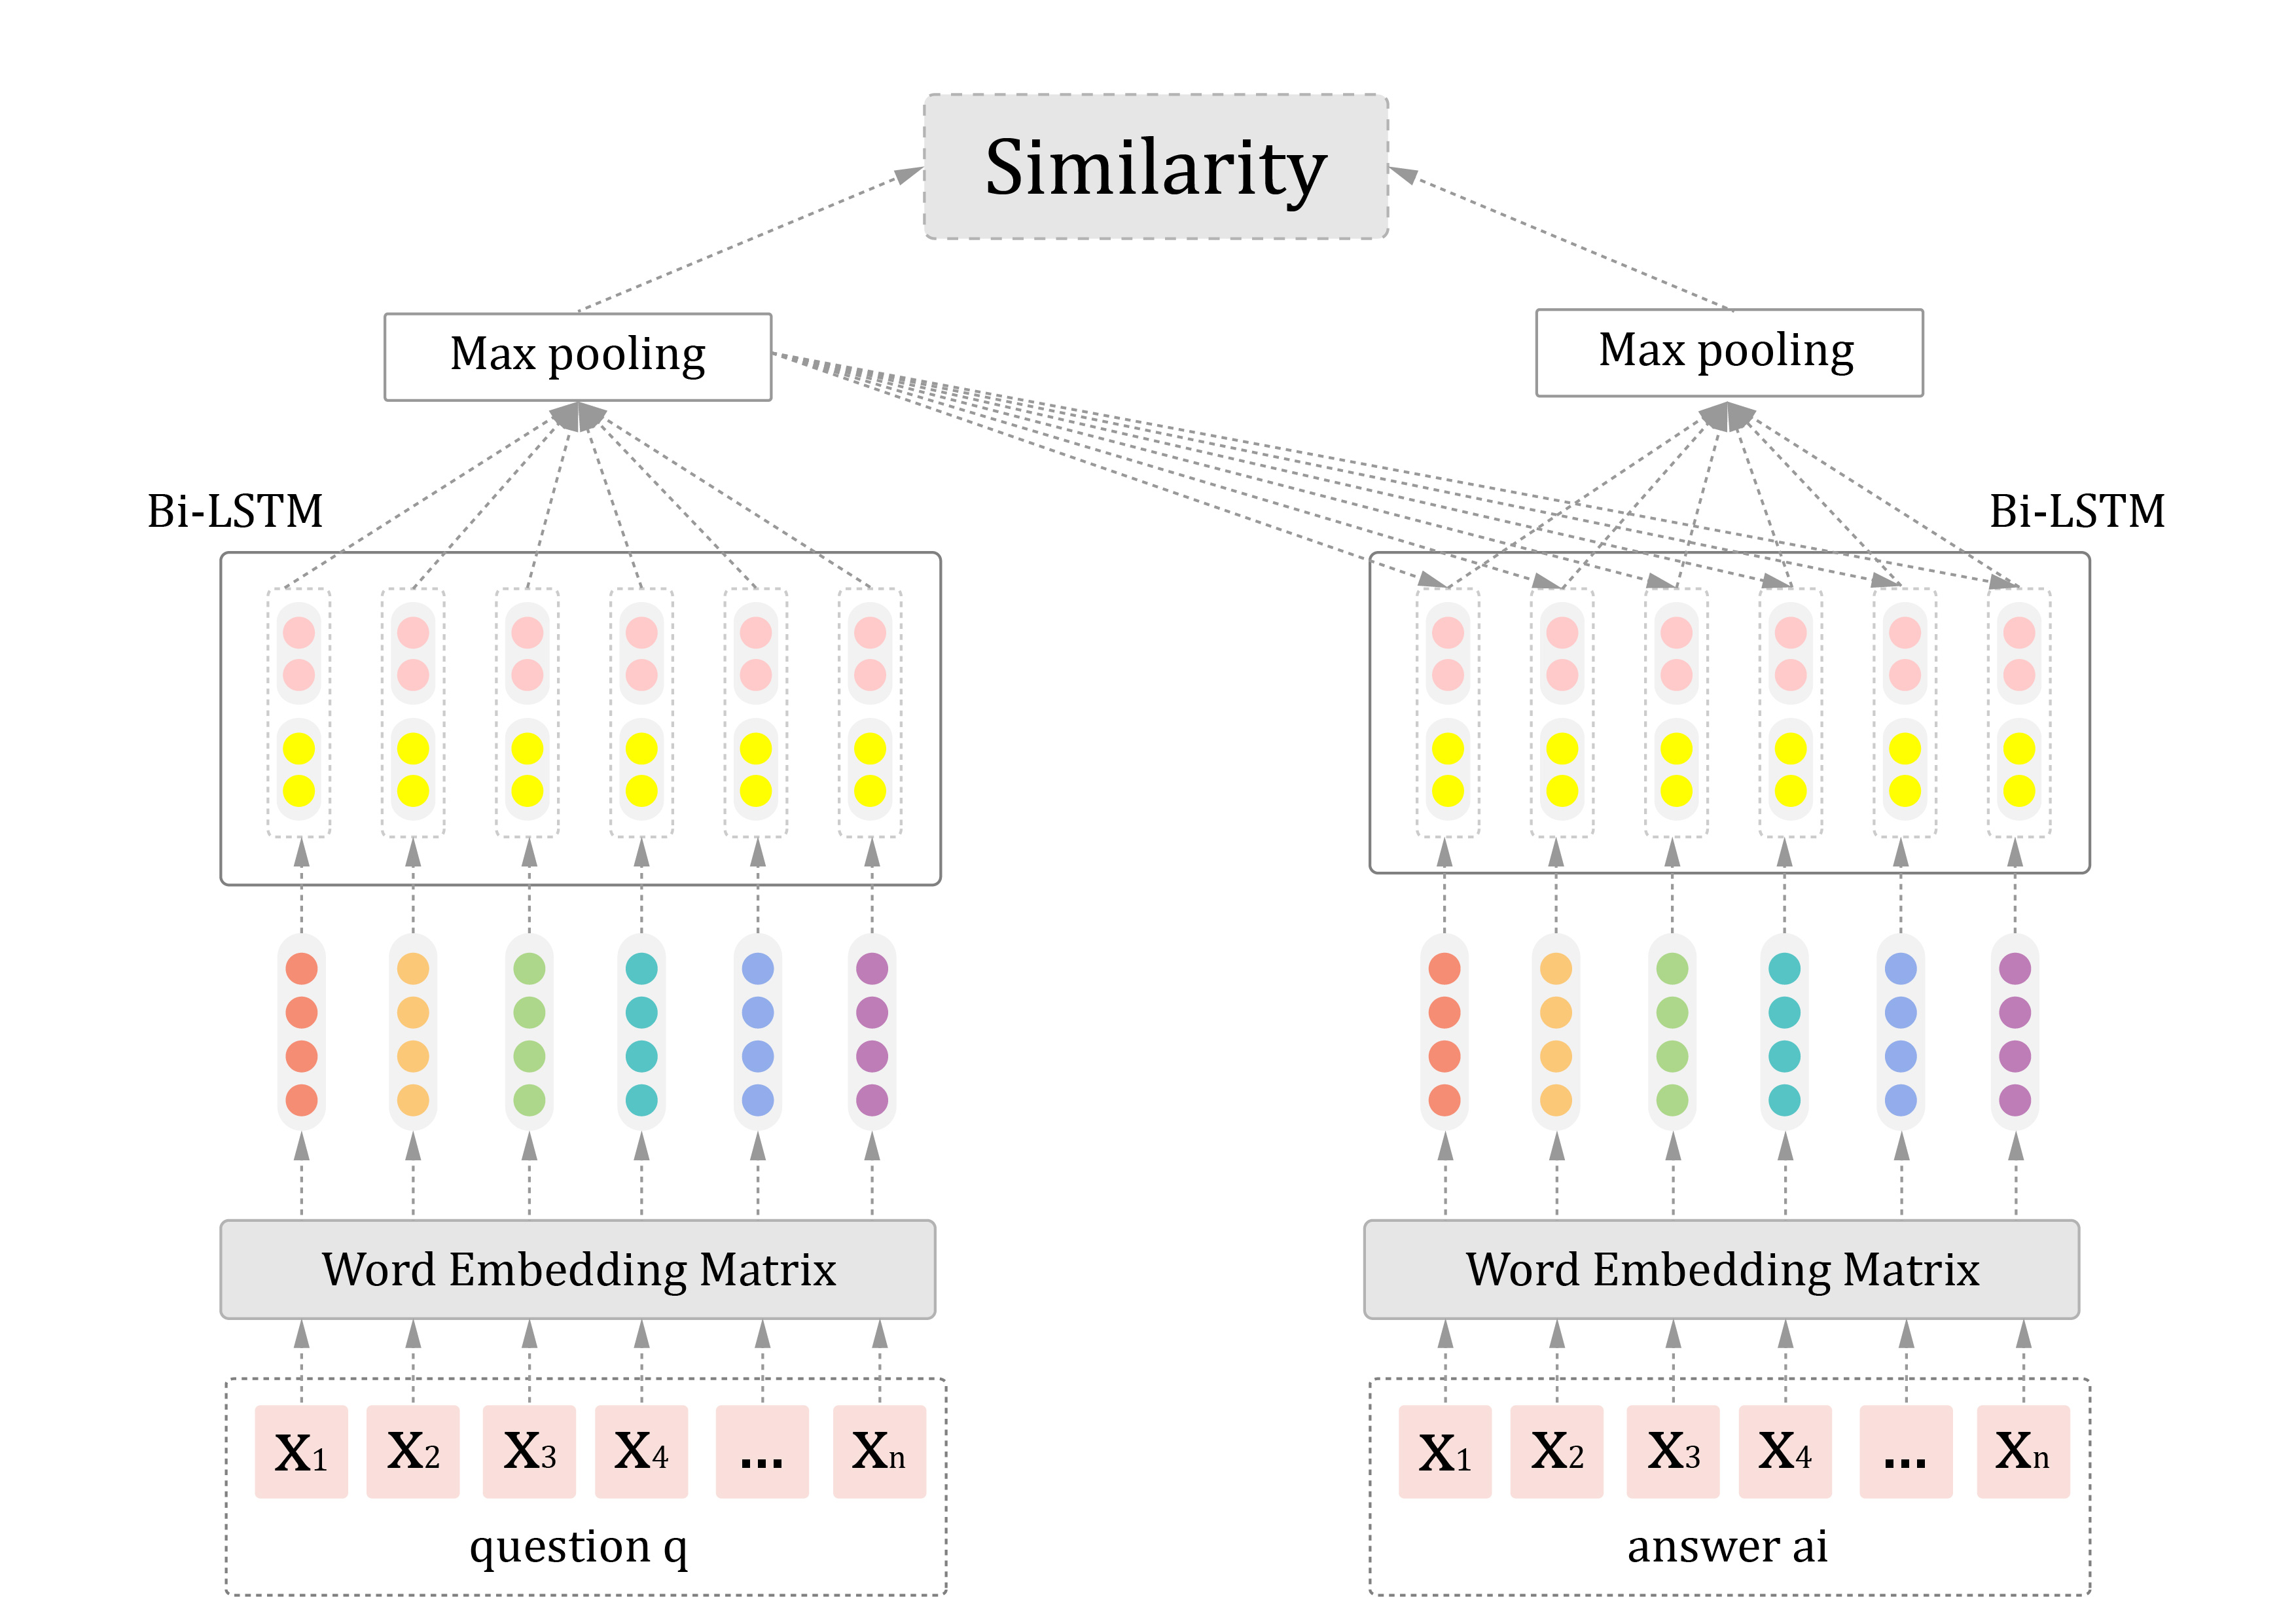
\includegraphics[height=8cm]{resource/qa_bi_lstm}
	\caption{基于Bi-LSTM的问题、答案表示模型}
	\label{fig:qa_bi_lstm}
\end{figure}

 首先生成问题、答案词序列的初始词向量, 然后输入到 Bi-LSTM 网络进入训练,得到问题和答案的最终向量表示, 最后词向量做 max pooling 后通过余弦相似性计算问题、答案向量 矩阵的相关性。实验设置问题、答案的 Bi-LSTM 网 络共享参数, Feng[24]等人的研究表明两个网络共享 参数较两个网络拥有各自不同参数性能更优。
 \\
 
 $\P$基于注意力机制的答案表示
 
与上述模型单独对问题和答案进行表示不同,此节使用一种基本的注意力机制模型,答案中每个词的向量生成均依赖问题,通过动态地将答案中更多的有效信息与问题对齐,可以更好的表示答案与问题之间的依赖关系。 此该注意力机制已在许多自
然语言处理任务上取得不错效果,如机器翻译[25]、事实型问答[26]、句子摘要[20]等。

图 4 为本文基于注意力机制的答案表示模型,模型使用词级别的注意力,如图中描述,在答案端Bi-LSTM 网络输出进入 max pooling 层之前,每个输出会乘以一个基于句子的 Attention 值。 时间 t 时刻, 令答案端的 Bi-LSTM 输出向量为 ,问题词向量为$\textbf{o}_q$,答案中每个词向量$\tilde{\textbf{h}}_{a}(t)$更新如下:
$$
\textbf{m}_{a,q}(t) = \tanh(\textbf{W}_{am}\textbf{h}_{a}(t) + \textbf{W}_{qm}\textbf{o}_q)
\eqno(8)
$$
$$
s_{a,q}(t) = softmax(\textbf{w}_{sm}\textbf{m}_{a,q}(t))
%s_{a,q}(t) = softmax(\textbf{w}_{sm} \tanh(\textbf{W}_{am}\textbf{h}^{a}_t + \textbf{W}_{qm}\textbf{o}_q))
\eqno(9)
$$
$$
\tilde{\textbf{h}}_{a}(t) = \textbf{\textbf{h}}_{a}(t) s_{a,q}(t)
\eqno(10)
$$

其中,$\textbf{W}_{am}$、$\textbf{W}_{qm}$为注意力机制参数矩阵,$\textbf{w}_{sm}$为注意力机制参数向量。从直观上看, 运用注意力机制表示答案相当于一定程度上将答案中与问题关键词相似的词增加权重,给无关词减少权重,使更易于区分正确答案和错误答案。

\begin{figure}[!htb]
	\centering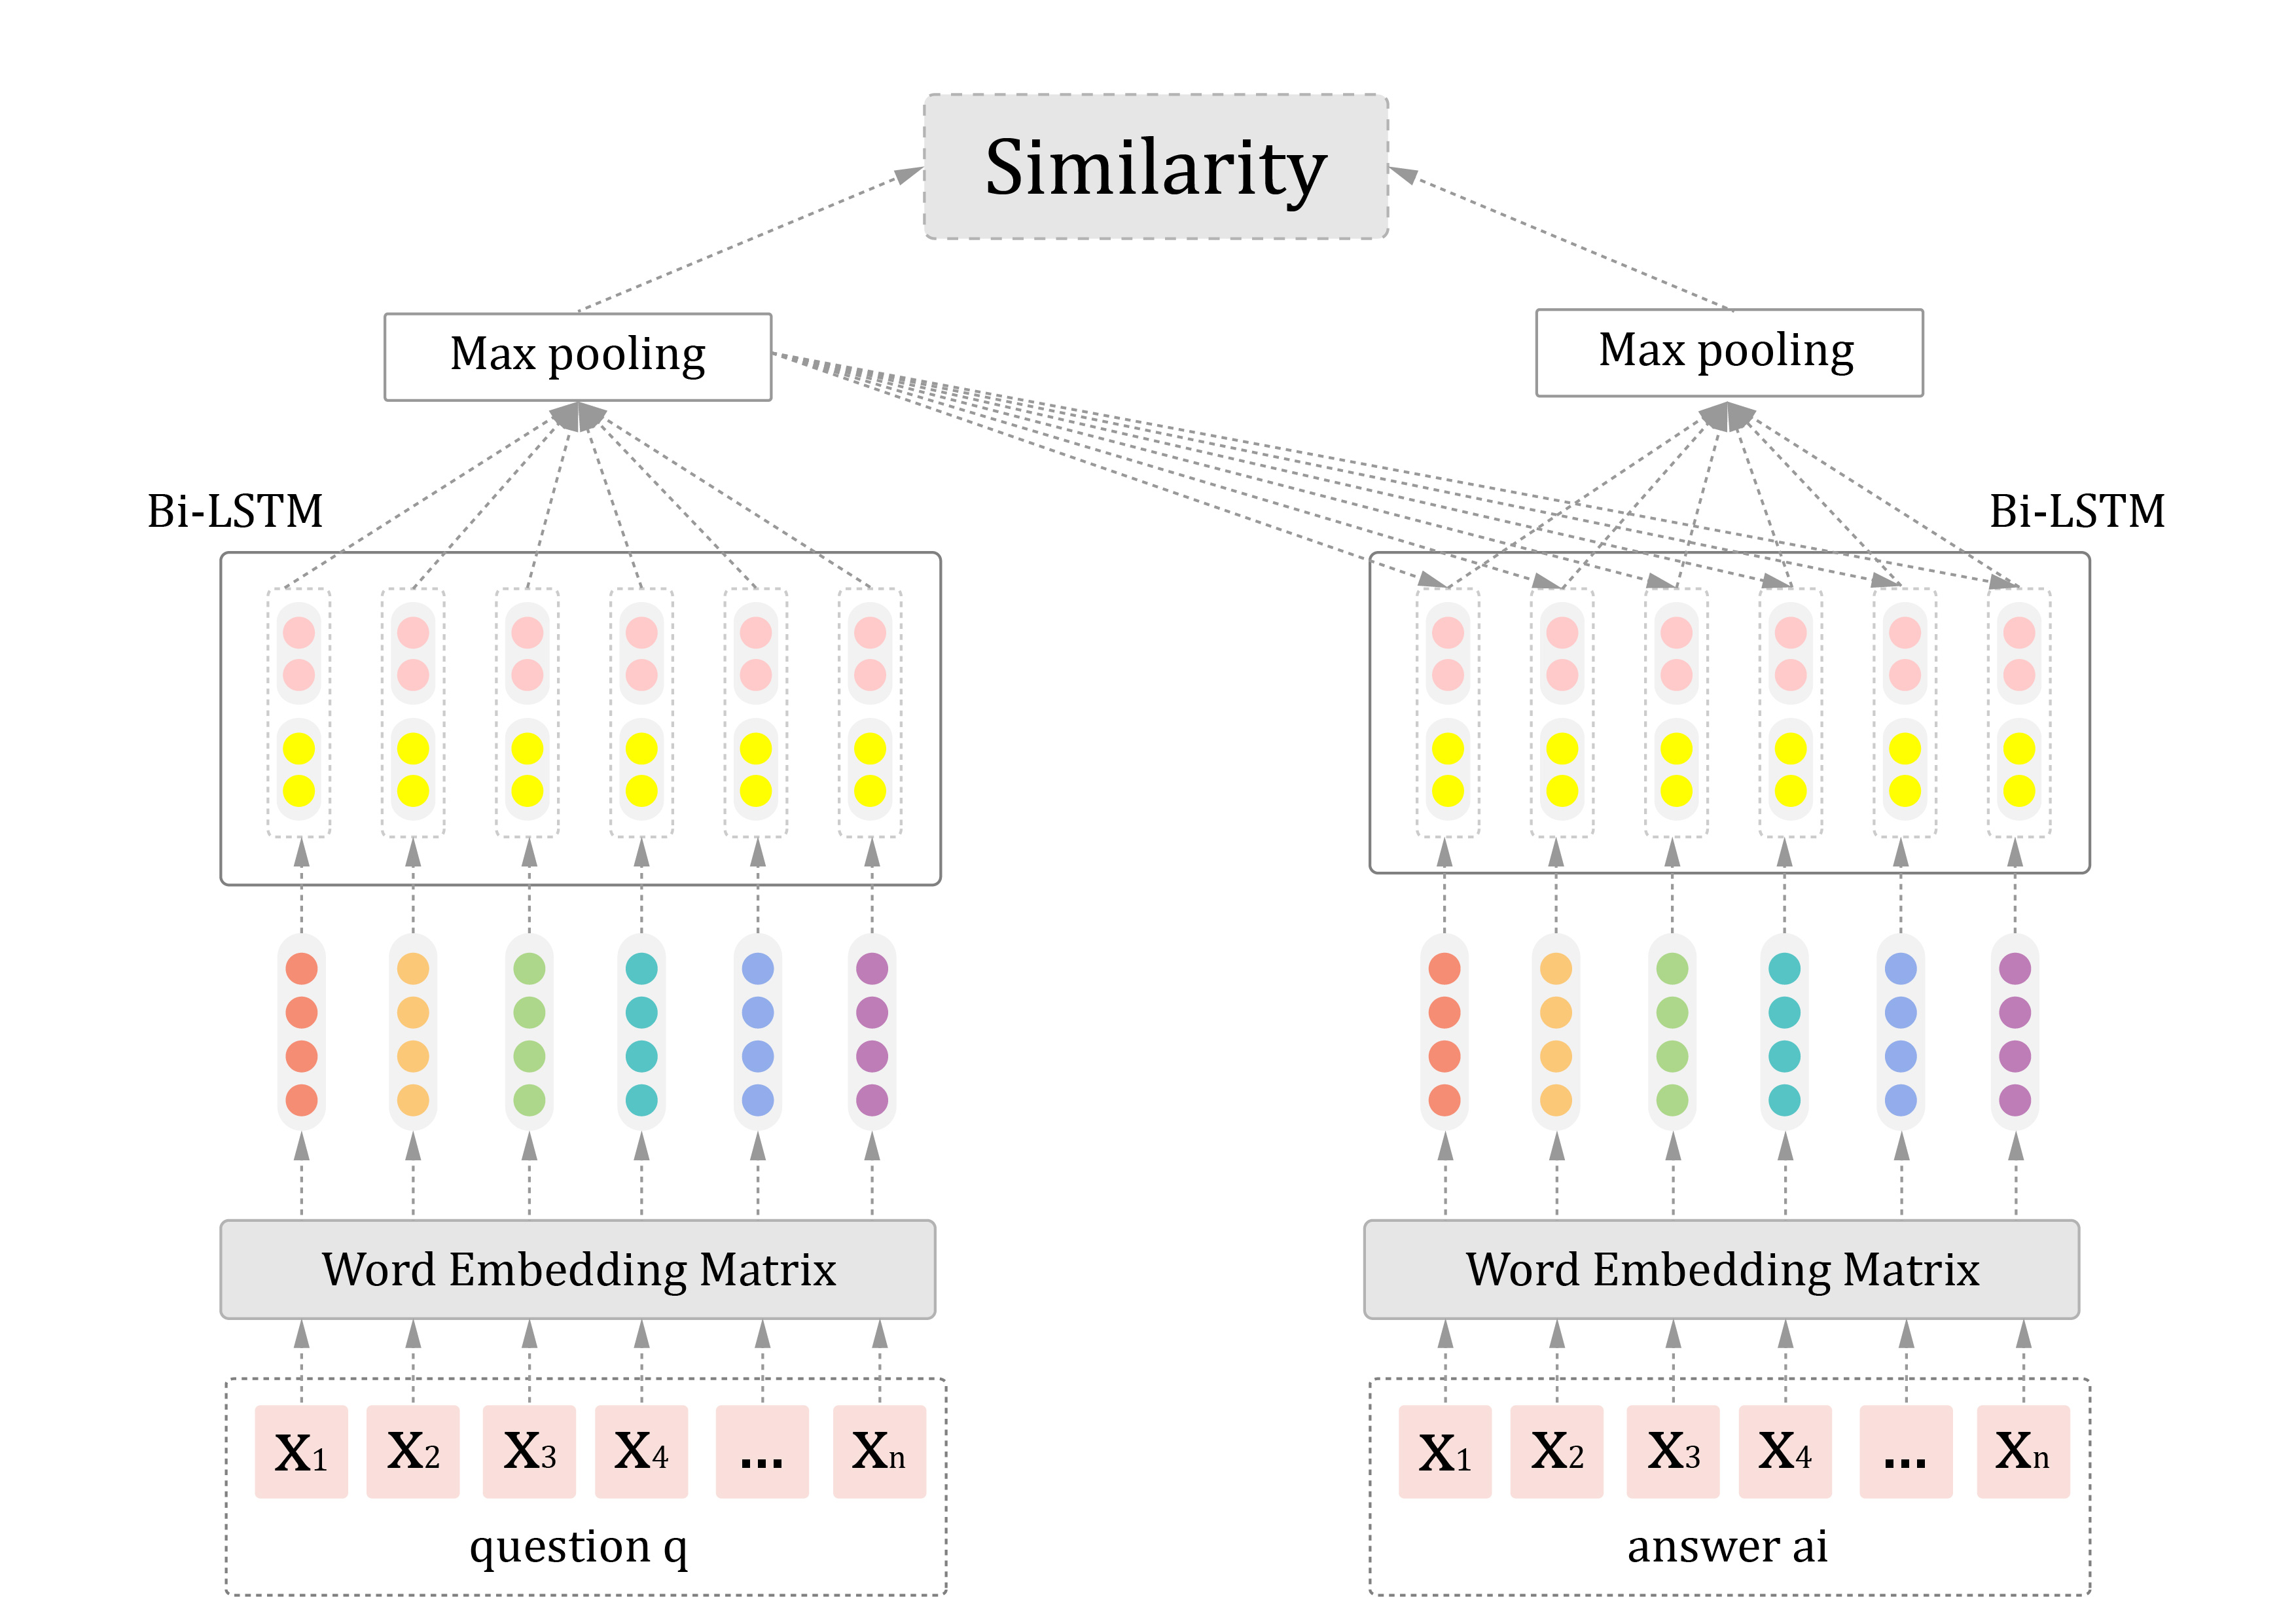
\includegraphics[height=8cm]{resource/qa_attention}
	\caption{基于Attention机制的问题、答案表示模型}
	\label{fig:qa_attention}
\end{figure}


\subsubsection{模型训练}
本文采取问答常见的问答对训练方式(Pairwise Training[27]),训练数据形式为(问题、正确答案、错误答案)。对于某个问题,本文选取一个正确答案作为正例,同时选取k个错误答案作为负例,负例的选择一部分来自主题实体的非答案三元组,另一部分随机从其他问题的正确答案中选取。损失函数使用铰链损失函数(hinge loss),如下:
 $$
\mathcal{L}(q, a_+, a_-) = max \{0, m - S(q, a_+) + S(q, a_-)\}
\eqno(11)
$$

m为正确答案得分和错误得分差距,S(.)为余弦函数,$a_+$为问题的正确答案,$a_-$为问题的错误答案。目标函数为:

$$
\min \sum_q\frac{1}{|P_q|}\sum_{a_+ \in P_q}\sum_{a_- \in N_q} \mathcal{L}(q, a_+, a_-)
\eqno(12)
$$

其中$|P_q|$为问题q的正确答案个数,$N_q$为问题q的k个错误答案集合。本文采取随机梯度下降(stochastic gradient descent,SGD)学习算法。


\subsubsection{最终答案选取策略}
在测试阶段,问答模型给所有候选答案打分排序,然后选择出得分最高答案三元组$S_{max}$,考虑到一个问题的正确答案可能不止一种,因此,本文设置答案阈值,此阈值取损失函数中的m,将得分与最高分相差不超过m的三元组也视作最终答案。如下:$\widehat{A_q}$为最终答案集合,$\hat{a}$为候选答案。
$$
S_{max} = \arg\max_{a \in C_q}{S(q,a)}
\eqno(13)
$$
$$
\widehat{A_q} = \{\hat{a}|S_{max} - S(q, \hat{a}) < m\}
\eqno(14)
$$

\subsection{地理问答实验}
为了评估实验模型,本文使用863项目组构建的基础知识库,同时为了解决目前中文地理领域问题缺乏的问题,本文又构建了较大规模的地理问题测试集,详细在本章数据集小结讲述。先介绍实验相关设置,然后介绍实验结果以及实验分析,最后介绍地理数据集的生成过程。
\subsubsection{参数设置}
实验词向量由word2vec[28]结合最新的中文维基百科语料训练得到,词向量维度为300。实验采取随机梯度下降优化策略,实验尝试过不同的m值,如0.1、0.2、0.3,最终选择0.1。学习率初始值为0.4,每10个epochs下降50$\%$,总共下降4次。剪枝参数max\_grad\_norm设为5,dropout取1.0。实验batch\_size取50,问题负例个数k取20,问题和答案的最大长度设置为50,超出最大长度内容舍弃,双向LSTM隐藏单元长度设为200。

\subsubsection{评价指标}
本文地理知识库问答实验采用知识库问答任务中常用的评价指标:平均倒数排序(Mean Reciprocal Rank,MRR )、准确率Accuracy@N【段】。如下为两个指标的定义:

$$
MRR = \frac{1}{|Q|}\sum_{i=1}^{|Q|}\frac{1}{rank_i}
\eqno(15)
$$
公式(15)中$|Q|$表示评估集中问题总数,$rank_i$表示当前问题的候选答案生成集中正确答案的位置,其中候选答案生成集是按照答案打分降序排序。若候选答案生成集中没有包括正确答案,则$rank_i$的值设为0。
$$
Accuracy@N = \frac{1}{|Q|}\sum_{i=1}^{|Q|}\delta(C_i, A_i)
\eqno(16)
$$
公式(16)中$|Q|$表示评估集中问题总数,$\delta(C_i, A_i)$表示候选答案生成集中是否至少包含一个正确答案,若是,则$\delta(C_i, A_i)$值为1,否则,值为0。

\subsubsection{实验结果}
实验使用NLPCC2016中1000个问题和本文从互联网抓取的436个地理问题(问题持续人工筛选中)进行测试,分别对本文方法章节中模型进行实验,问答评价指标使用MRR和Accuracy@N,实验结果如表\ref{tab:qa_expriment}所示:
%{lcl}
\begin{table}[htbp] 
	\centering
	\caption{\label{tab:qa_expriment}地理问答实验结果} 
	\begin{tabular}{lcl}
		\toprule 
		Method	&      MRR & Accuracy@N \\
		\midrule 
		LSTM & 0.809 & 0.847 \\ 
		Bi-LSTM & 0.821 & 0.868 \\ 
		\textbf{Bi-LSTM + Attention} & \textbf{0.834} & \textbf{0.872} \\ 
		\bottomrule 
	\end{tabular} 
\end{table}

\subsubsection{实验分析}
由表中实验结果可知,Bi-LSTM相对单向LSTM的MRR、Accuracy@N分别提高了1.2$\%$、2.1$\%$,说明Bi-LSTM相比LSTM能表示问题能力更强。同时基于注意力机制的Bi-LSTM比单纯的Bi-LSTM两个指标分别提升1.3$\%$、0.4$\%$,加入Attention后问答MRR指标提升比较明显,说明本文注意力机制可以更准确的区分比较相似的答案。

\subsubsection{地理问答数据集构建}
\subsection{结论}









在给定指称项$m$和指称项对应的候选实体集$E_m=\{e_1,e_2,...,e_n\}$后,计算模型的输入特征:

\begin{enumerate}
	\renewcommand{\labelenumi}{(\theenumi)}
	\item {候选实体$e_i$在知识库中的先验概率,$PriorInKB(m,e_i)$,该特征的定义如公式\ref{eq:popinkb}所示。
		
		\begin{equation}\label{eq:popinkb}
		PriorInKB(m,e_i)=\frac{count(e_i)}{\sum_{e_i\in E_m} {count(e_k)}}
		\end{equation}
		
		其中,$count(e)$表示实体$e$在知识库中作为锚文本出现的次数。
	}
	\item {指称项上下文与候选实体对应词条摘要的文 本相似度,$ContextSimilarity(m,e_i)$,该特征的定义如公式\ref{eq:contex_similarity}所示。
		
		\begin{equation}\label{eq:contex_similarity}
		ContextSimilarity(m,e_i)=\frac{coocurence(m,e_i)}{length(m)}
		\end{equation}
		
		其中,$coocurence(m,e_i)$表示指称项$m$上下文和候选实体$e_i$对应知识库中摘要文本相同的单词数,$length(m)$表示指称项$m$的上下文长度。
	}
	\item {带标注样本集中,候选实体$e_i$的流行度,$PopInCorpus(e_i)$,该特征会随着人工标注的进行而产生变化。该特征的定义如公式\ref{eq:pop_in_corpus}所示。
		
		\begin{equation}\label{eq:pop_in_corpus}
		PopInCorpus(e_i)=\frac{\sum_{anno \in Corpus} {I(anno.e,e_i)}}{sizeof(Corpus)}
		\end{equation}
		
		其中,$anno$表示已标注语料中的一条标注记录,$anno.e$表示标注记录的目标实体。$I(e_i,e_j)$是示值函数,实体$e_i$和实体$e_j$相同则为1,否则为0。$sizeof(Corpus)$表示已标注指称项个数。
	}
	\item{带标注样本集中,候选实体$e_i$作为指称项$m$的目标实体的先验概率,$Prior(m,e_i)$,同上,该特征也会随着标注的进行而产生变化。该特征的定义如公式\ref{eq:prior}所示。
		
		\begin{equation}\label{eq:prior}
		Prior(m,e_i)=\frac{\sum_{anno \in Corpus} {I(anno.e,e_i)\times I(anno.m,m)}}{\sum_{anno \in Corpus} {I(anno.m,m)}}
		\end{equation}
		
		其中,$anno.e$的定义同上。$anno.m$表示标注记录$anno$的指称项。
	}
	\item 指称项名字和候选实体标题的编辑距离,$EDSimarity(m,e_i)$。该特征的定义如公式\ref{eq:ed_simarity}所示。
	
	\begin{equation}\label{eq:ed_simarity}
	EDSimarity(m,e_i)=
	\left\{
	\begin{array}{rcl}
	1       &      & {|length(m)-length(e_i)|=ED(m,e_i)}\\
	0    &      & {\text{其它}}
	\end{array} \right.
	\end{equation}
	
	编辑距离$ED(\cdot,\cdot)$是指两个字符串进行转换时,需要的字符级最少操作次数。编辑距离相似度能够检测指称项和候选实体之间的别名、缩略名等关系。
\end{enumerate}

\subsection{目标实体预测}
在使用监督学习模型$C$处理实体链接任务时,首先需要训练模型$C$。训练样本由带标注的指称项集合构成,例如,带标注的指称$m$包含$n$个候选实体,指称$m$的目标实体是$e^*$,任意一个候选实体$e_i$和指称项$m$组成一 个样本对$\left\langle m,e_i\right\rangle $,若$e_i$是目标实体$e^*$,样本对标记为正例,否则标记为反例。用所有带标注的样本对训练得到模型$C$。

训练得到模型$C$后,对于未标注指称$m$及其候选实体集$E_m$,根据上一节的计算方法获得所有候选实体和指称项组成的样本对的特征向量,模型$C$根据输入的特征向量,计算每个候选实体是目标实体的概率$P_C(e_i|m)$。该预测概率的计算方式和模型的选择相关,例如选择支持向量机模型,可以用样本点距离分类超平面的距离估计正确分类的概率\cite{李航2012统计学习方法};选择人工神经网络模型,可以对输出层每个节点的权值做$softmax$处理,以此获得每个分类标签的分类预测概率\cite{ravuri2016comparative},在此不再一一例举其它模型的预测概率估计方法。取概率最高的候选实体作为指称项$m$的预测实体,如公式\ref{eq:hat_cancidate}所示。

\begin{equation}\label{eq:hat_cancidate}
\hat{e}=\argmax_{e_i\in E_m} P_C(e_i|m)
\end{equation}

然后将该预测实体被正确划分的概率作为指称$m$被正确链接的概率,如公式\ref{eq:predict_prob}所示。

\begin{equation}\label{eq:predict_prob}
P_C(\hat{e}|m)=\max_{e_i\in E_m}P_C(e_i|m)
\end{equation}

\section{实体链接的主动学习算法}
为了减少人工标注的工作量,本文采用基于池的主动学习方法(Pool-based Active Learning)选择实体链接的待标注指称项。主动学习流程图如图\ref{fig:al_overview}所示。

\begin{figure}[!htb]
	\centering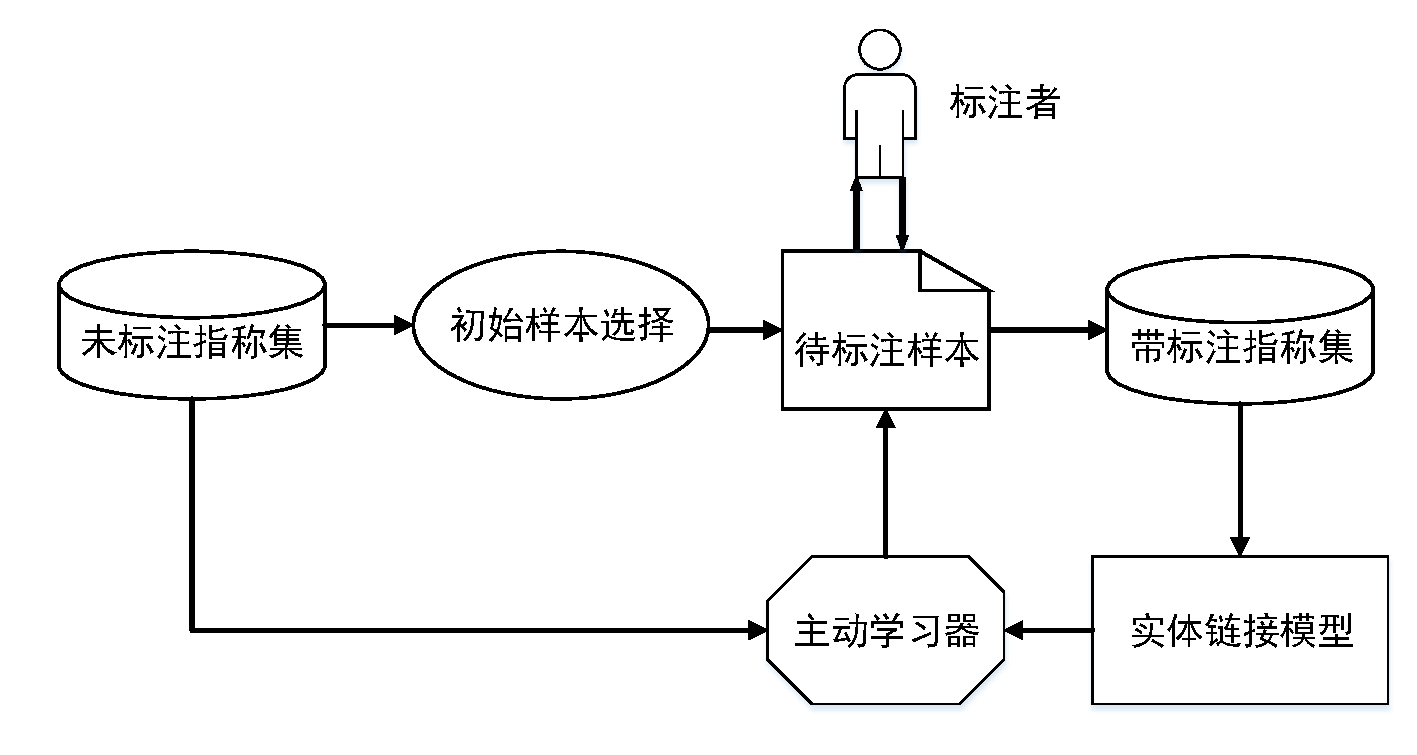
\includegraphics[height=7cm]{resource/al_overview}
	\caption{主动学习流程概览}
	\label{fig:al_overview}
\end{figure}

在每轮迭代训练中,主动学习器能够选出信息量最大的未标注样本集交由人工标注。已有的主动学习\cite{settles2012active}流程如算法\ref{algorithm_AL}所示。在给定未标注训练样本集后, 主动学习进程分为两个阶段,第一阶段的工作是选择初始训练样本集并以此训练初始分类器,第二阶段的工作是选择最佳标注样本并以此迭代训练模型。

\floatname{algorithm}{算法}
\renewcommand{\algorithmicrequire}{\textbf{输入:}} % Use Input in the format of Algorithm
\renewcommand{\algorithmicensure}{\textbf{输出:}} % Use Output in the format of Algorithm
\begin{algorithm}[!htb]
	\caption{基于主动学习的实体链接任务训练进程}
	\label{algorithm_AL}
	\begin{algorithmic}[1] %这个1 表示每一行都显示数字
		\REQUIRE ~ %算法的输入参数:Input
		未标注的指称样本集$ \mathcal{U}=\{m^{(u)} \}_{u=1}^U $
		\ENSURE ~ %算法的输出:Output
		实体链接分类器$C$
		\STATE 从未标注训练集$\mathcal{U}$中选择并标注初始训练样本集$\mathcal{L}_0$\label{al_sup_line1}
		\STATE 利用初始训练样本集$\mathcal{L}_{0}$训练得到弱分类器$C=train(\mathcal{L}_{0})$\label{al_sup_line2}
		\REPEAT \label{al_sup_line3}
		\STATE 从$\mathcal{U}$中找出$k$个信息量最大的样本组成样本集$ \mathcal{U}_{selected} = \{m^{(u)} \}_{u=1}^{k} $\label{al_sup_line4}
		\STATE 对$ \mathcal{U}_{selected}$中的指称进行人工标注得到$ \mathcal{L}_{selected} = \{\left\langle m,e\right\rangle^{(l)} \}_{l=1}^{k} $
		\STATE $ \mathcal{U} = \mathcal{U} \setminus \mathcal{U}_{selected} $
		\STATE $ \mathcal{L}_{t+1} = \mathcal{L}_{t} \cup \mathcal{L}_{selected} $
		\STATE $C=train(\mathcal{L}_{t+1})$
		\UNTIL {达到预期精度或样本集已全部标注} \label{al_sup_line9}
		\RETURN $C$
	\end{algorithmic}
\end{algorithm}

算法第\ref{al_sup_line1}-\ref{al_sup_line2} 行对应主动学习进程的第一个阶段,已有的做法是在未标注样本集$\mathcal{U}$中随机选择待标注样本$\mathcal{U}_{selected}$,然后对这些未标注样本进行人工标注,通过这种方式得到初始带标注样本集$\mathcal{L}_0$,然后用$\mathcal{L}_0$训练得到初始实体链接模型$C$。由于当初始带标注样本集合较小时,通过随机选择的方式获得的子样本集可能无法很好地代表整个样本集。因此,本文对初始训练样本选择方法做了改进,提出基于指称项流行度的初始样本选择方法。

算法第\ref{al_sup_line3}-\ref{al_sup_line9} 行对应主动学习的第二个阶段,其中对于算法第\ref{al_sup_line4}行 信息量度量方法的选择,已有的做法是将样本分类结果的不确定度大小作为信息量的衡量标准,第$t$轮迭代中选出的样本会被加入到带标注样本集$\mathcal{L}_t$中,然后用$\mathcal{L}_t$重新训练模型。在实体链接任务中,仅将不确定度作为选择待标注样本的依据,可能会导致选择过多的离群样本点,不利于模型的训练。因此,本文对迭代训练样本选择方法做了改进,提出综合分类不确定度和指称项流行度的迭代训练样本选择方法。

\section{改进的初始训练样本选择方法}\label{section:al_init_gen}
本节首先对改进的初始训练样本选择方法进行了详细说明,然后给出了该方法对应的算法描述。

\subsection{初始训练样本选择方法}
在主动学习的初始阶段,需要产生一个初始样本集用于训练初始模型。已有的主动学习方法采用随机选择的方式产生初始训练样本集,由于训练样本集相对较小,随机选择的方式很难保证初始样本集的代表性。但是,训练一个性能较好的初始模型对提高主动学习收敛速度非常重要。因此,本文对已有的基于随机选择的初始样本集生成方法做了改进。

为了提高实体链接初始模型的性能,本文提出基于流行度的初始样本选择方法(Sampling by Popularity, SBP)。指称项的流行度按照相同名字的指称项在语料库中出现的频率计算。例如,语料库中包含$n$个指称项,名字为“Jordan”的指称项出现了$m$次,则名字为“Jordan”的所有指称项的流行度为$m/n$。该样本选择方法首先对指称项按照指称项名字分类,计算指称项流行度,然后对指称项流行度高的样本做标注,加入初始训练样本集。该方法的目的是在初始样本选择阶段,尽量选择出现频率较高的指称项,以此保证初始样本集的代表性,从而提高在初始样本集较小的情况下,尽可能提高初始模型的性能。

\subsection{初始训练样本选择算法}
算法\ref{algorithm_init}是对基于流行度的初始样本选择方法的算法描述。初始训练样本的选择分为两个步骤,第一步是不同指称项流行度的统计;第二步是根据指称项流行度选择初始训练样本。

算法第\ref{al_init_line1}-\ref{al_init_line2}行对未标注样本集按指称项名字进行分类,例如所有指称名字为“Jordan”的训练样本都会被划分到集合$\Psi_{Jordan}$中。然后根据集合中的样本数量计算各个指称项在训练集中的流行度,指称项名字相同的样本具有相同的流行度。

算法第\ref{al_init_line3}-\ref{al_init_line7}行对指称项流行度做排序,并在流行度最高的$k$个样本集中分别随机选择一个或多个\footnote{当指称名字数量小于$k$时,需要在一个类簇中选择多个样本,保证最终获得$k$个样本。}样本,经过人工标注后加入初始训练样本集。这样做的目的在于避免初始训练样本集中的样本指称项名字重复度过高,同时保证尽量选择流行度高的指称项样本,从而提高初始训练样本集的代表性。

\floatname{algorithm}{算法}
\renewcommand{\algorithmicrequire}{\textbf{输入:}} % Use Input in the format of Algorithm
\renewcommand{\algorithmicensure}{\textbf{输出:}} % Use Output in the format of Algorithm
\begin{algorithm}[!htb]
	\caption{基于流行度的初始样本集选择算法}
	\label{algorithm_init}
	\begin{algorithmic}[1] %这个1 表示每一行都显示数字
		\REQUIRE ~ %算法的输入参数:Input
		未标注的实体链接样本集$ \mathcal{U}=\{m^{(u)} \}_{u=1}^U $,初始训练集样本个数$k$
		\ENSURE ~ %算法的输出:Output
		初始样本集$\mathcal{L}$
		\STATE 对未标注训练样本按照指称名字$name$分组,指称名字为$name$的样本被分到集合$\Psi_{name}$中\label{al_init_line1}
		\STATE 计算名字为$name$的指称的流行度$\Phi_{name}=\frac{|(\Psi_{name})|}{U}$\label{al_init_line2}
		\STATE 对不同指称的流行度排序,取流行度最高的$k$个指称的名字\label{al_init_line3}
		
		$\mathcal{S}=\{name_1,name_2,...,name_k\}$\label{al_init_line4}
		\FOR {each $name$ in $\mathcal{S}$}
		\STATE 从集合$\Psi_{name}$中随机取一个或多个样本并对其人工标注得到带标注的样本对$L=\left\langle m,e\right\rangle$\label{al_init_line5}
		\STATE $\mathcal{L}=\mathcal{L} \cup \{L\}$
		\ENDFOR\label{al_init_line7}
		\RETURN $\mathcal{L}$
	\end{algorithmic}
\end{algorithm}

\section{改进的迭代训练样本选择方法}\label{section:al_iter_train}
本节首先对改进的迭代训练样本选择方法进行了详细说明,然后给出了该方法对应的算法描述。

\subsection{迭代训练样本选择方法}
在初始训练集上训练得到初始模型后,需要迭代选择信息量最大的未标注样本做标注,然后对模型做重新训练。在已有的主动学习迭代训练样本选择过程中,通常将不确定度最大的样本作为信息量最大的样本,这些样本会交由人工标注并加入下一轮迭代训练,通过这种方式迭代逼近真实模型。本文采用间隔(Margin)度量未标注样本的不确定度。

如公式\ref{eq:margin_confidence}所示 ,$e^{*1}$和$e^{*2}$分别表示在当前模型$C$中,给定指称项$m$,对应置信度最高的和次高的候选实体,以这两个候选实体的置信度差的绝对值作为指称$m$链接到正确实体的置信度。

\begin{align}\label{eq:margin_confidence}
\begin{aligned}
Confidence(m)&=P_C(e^{*1})-P_C(e^{*2})\\
\text{其中,\quad\quad\quad\quad\quad\quad\quad\quad\quad\quad\quad\quad}&\text{\quad\quad\quad\quad\quad\quad\quad\quad\quad\quad\quad\quad\quad\quad\quad\quad}\\
e^{*1}&=\argmax_{E_i\in E_m}P_C(e_i|m)\\
e^{*2}&=\argmax_{E_i\in E_m \setminus \{e^{*1}\}} P_C(e_i|m)
\end{aligned}
\end{align}

易知,$Confidence(m)$越小,表示模型$C$越难正确地从候选实体$e^{*1}$和候选实体$e^{*2}$中区分出目标实体,因此,指称项$m$被正确链接的置信度越小,指称项被正确链接的不确定度越大。指称项链接的不确定度如公式(\ref{eq:margin_uncertainty})所示。

\begin{equation}\label{eq:margin_uncertainty}
Uncertainty(m)=1-Confidence(m)\\
\end{equation}

在本文的实体链接任务中,如果采用仅基于不确定度的样本选择方法来选择待标注样本,则会存在两个缺陷。第一,存在一些不确定度较大,但是在所有样本中处于边缘位置的样本,这些离群样本点不具有代表性,相反还可能会对模型的训练产生负作用,在样本选择过程中,应该尽量避免这类样本点;第二,本文实体链接模型的输入特征向量包含已标注语料中候选实体流行度($PopInCopus(e_i)$)和已标注语料中候选实体先验概率($Prior(e_i|m)$)这两个特征维度,这两个特征都是在已标注样本集上通过统计得到的,因此,带标注的样本分布越离散,带标注样本集中包含的指称项和实体越多,那么上述两个特征维度的统计量越具有代表性。从这个角度看基于不确定度的样本选择算法对这两个特征的计算可能会产生负面影响。因此主动学习的样本选择策略需要在不确定度和多样性之间取一个权衡。为了解决这个问题,本文提出综合不确定度和流行度的样本选择方法(Sampling by Uncertainty and Popularity, SUP)。

\subsection{综合不确定度和流行度的样本选择算法}
接下来给出综合不确定度和流行度的样本选择方法的算法描述。SUP算法是对不确定度和多样性的折衷,如算法\ref{algorithm_iter}所示。

\begin{algorithm}[htb]
	\caption{综合不确定度和流行度样本集选择算法}
	\label{algorithm_iter}
	\begin{algorithmic}[1] %这个1 表示每一行都显示数字
		\REQUIRE ~ %算法的输入参数:Input
		未标注的实体链接样本集$ \mathcal{U}=\{m^{(u)} \}_{u=1}^U $\\
		\quad \quad 选择标注的样本个数$k$
		\ENSURE ~ %算法的输出:Output
		本轮选择标注的训练样本集$ \mathcal{L} $\\
		\STATE $ \mathcal{L} = \{\} $
		\STATE 用K-means聚类法将未标注训练样本集按照指称的流行度划分为$k$类,$Clusters=\{\Psi_1,\Psi_2,...,\Psi_k\}$\label{al_iter_line2}
		\FOR {each $\Psi_i$ in $Clusters$}
		\STATE $m^{*}=\argmax_{m \in \Psi_i} Uncertainty(m)$\label{al_iter_line4}
		\STATE 对$m^{*}$人工标注,得到$\left\langle m^{*},e\right\rangle$
		\STATE $\mathcal{L}=\mathcal{L} \cup \{\left\langle m,e\right\rangle\}$
		\ENDFOR
		\RETURN $ \mathcal{L} $
	\end{algorithmic}
\end{algorithm}

算法第\ref{al_iter_line2}行将所有未标注样本集中的指称项按照指称项流行度进行聚类,完成聚类后,同一个类簇的样本流行度相近。

算法第\ref{al_iter_line4}行从各个流行度的类簇中分别选出不确定度最大的样本交由人工标注,这里不确定度的计算方式依然是模型预测的最优候选实体和次优候选实体置信度的间隔。该样本选择算法能够保证各个指称项流行度区间的样本都有均等机会被选中标注,同时又能保证在每个类簇中被选中标注的样本都是这个类簇中不确定度最大的样本,在兼顾所选样本集多样性的同时保证了不确定度。

\section{实验结果与分析}
本节介绍主动学习方法在实体链接模型训练中的实验,说明实验环境、实验所用数据集、评价指标以及实验配置,最后给出了实验结果数据,并对实验结果进行了分析。

\subsection{实验环境}\label{section:dev_env}
硬件环境:

\begin{itemize}
	\item CPU: Intel(R) Core(TM) i7-3770 CPU @ 3.40GHz
	\item Memory: 4$\times$8GB DDR3 1333 ECC
\end{itemize}

软件环境:

\begin{itemize}
	\item CentOS Linux release 7.3.1611 (Core)
	\item IntelliJ IDEA 2016.3
	\item Java 1.8
	\item MySQL 5.6
\end{itemize}

开源工具:

\begin{itemize}
	\item LibSVM\footnote{用于实现支持向量机。}
	\item Weka 3.6\footnote{用于配合LibSVM实现支持向量机训练。}
	\item Stanford NLP\footnote{用于实现英文分词及词干抽取。}
\end{itemize}

\subsection{实验数据集}\label{section:dataset}
本文使用的数据集是在\textit{CoNLL'03}的基础上做了实体链接标注的\textit{Aida}数据集。数据集包含 1393 篇文章和28815个可用指称项。本文取20000个指称项作为训练集,其余的指称项作为测试集。

\subsection{评价指标}
本章研究主动学习在实体链接模型训练中的作用,并验证本文提出的基于流行度的初始样本选择方法以及综合不确定度和流行度的迭代训练样本选择方法对减少人工标注样本工作量的效果。实际上数据集中的指称项都已经标注好对应的目标实体,但是在模型训练过程中,本文不直接使用 Aida 数据集的标注结果,只有通过主动学习方法选择的样本的标注结果才会被使用,以此来模拟人工标注的过程。本章实验分为以下两个方面:

(1) 以随机选择方法为基线方法,评价基于流行度的初始样本选择方法在标注相同数量样本的前 下,对初始模型性能提升的效果。

(2) 以随机选择法为基线方法,评价基于不确定度的样本选择方法以及综合不确定度和流行度的样本选择方法对模型训练收敛速度的提升效果。

本文对各种样本选择方法好坏的评价指标为主动学习过程中,由主动学习器选择的训练样本所训练得到的模型在测试集里的性能表现,性能表现体现在测试集上实体链接的正确率,计算方法如公式\ref{eq:sup_al_p}所示。

\begin{equation}\label{eq:sup_al_p}
\text{准确率}(P)=\frac{\text{测试集中被正确链接的指称项个数}}{\text{测试集中所有指称项个数}}\times 100\%
\end{equation}

\subsection{模型选择}
本章使用监督学习模型处理实体链接任务,并将该任务作为分类问题来处理。在常用的机器学习分类器中,SVM模型\cite{li2016linking}是目前分类效果较好的模型,其可以通过核函数(本文使用径向基函数(Radial Base Function, RBF))将非线性可分的输入空间的特征映射到高维线性可分的空间的特征,以此学习非线性可分模型。此外,样本点距离分类超平面的远近可以作为分类置信度的依据,而主动学习过程中,分类置信度恰好是样本选择策略的考虑因素之一。

综上,本文在实验阶段使用 SVM 模型作为监督学习模型的代表,处理实体链接任务并研究主动学习方法在该任务上发挥的作用。

\subsection{初始训练样本选择方法实验}
为了验证基于指称项流行度的初始训练样本选择方法对提高初始模型性能的效果,在实验环节,分别通过基于随机选择方法(Random)和基于流行度选择方法(SBP)得到初始样本集,对比在不同初始训练样本集大小的情况下,由初始样本集训练得到的初始模型的性能。

实验中,初始样本集大小的设置从 2000 开始,依次以 2000 递增,最大的初始样本集包含 18000 个训练样本。从图\ref{fig:al_sup_init_result}可以看出,在初始样本集较小的时候,基于指称项流行度的样本选择方法比随机样本选择方法在初始模型的性能上有显著的提升,在初始样本集大小为 2000 的时候,性能提升了 10.1\%,在初始样本集大小为 4000 的时候,性能提升了 5.3\%。当初始样本集大小继续增加时,性能提升值逐渐减小,甚至在一些情况下提升值为负。总体来看,当初始样本集较大时,两种初始训练样本选择方法性能差别不大。

\begin{figure}[!htb]
	\centering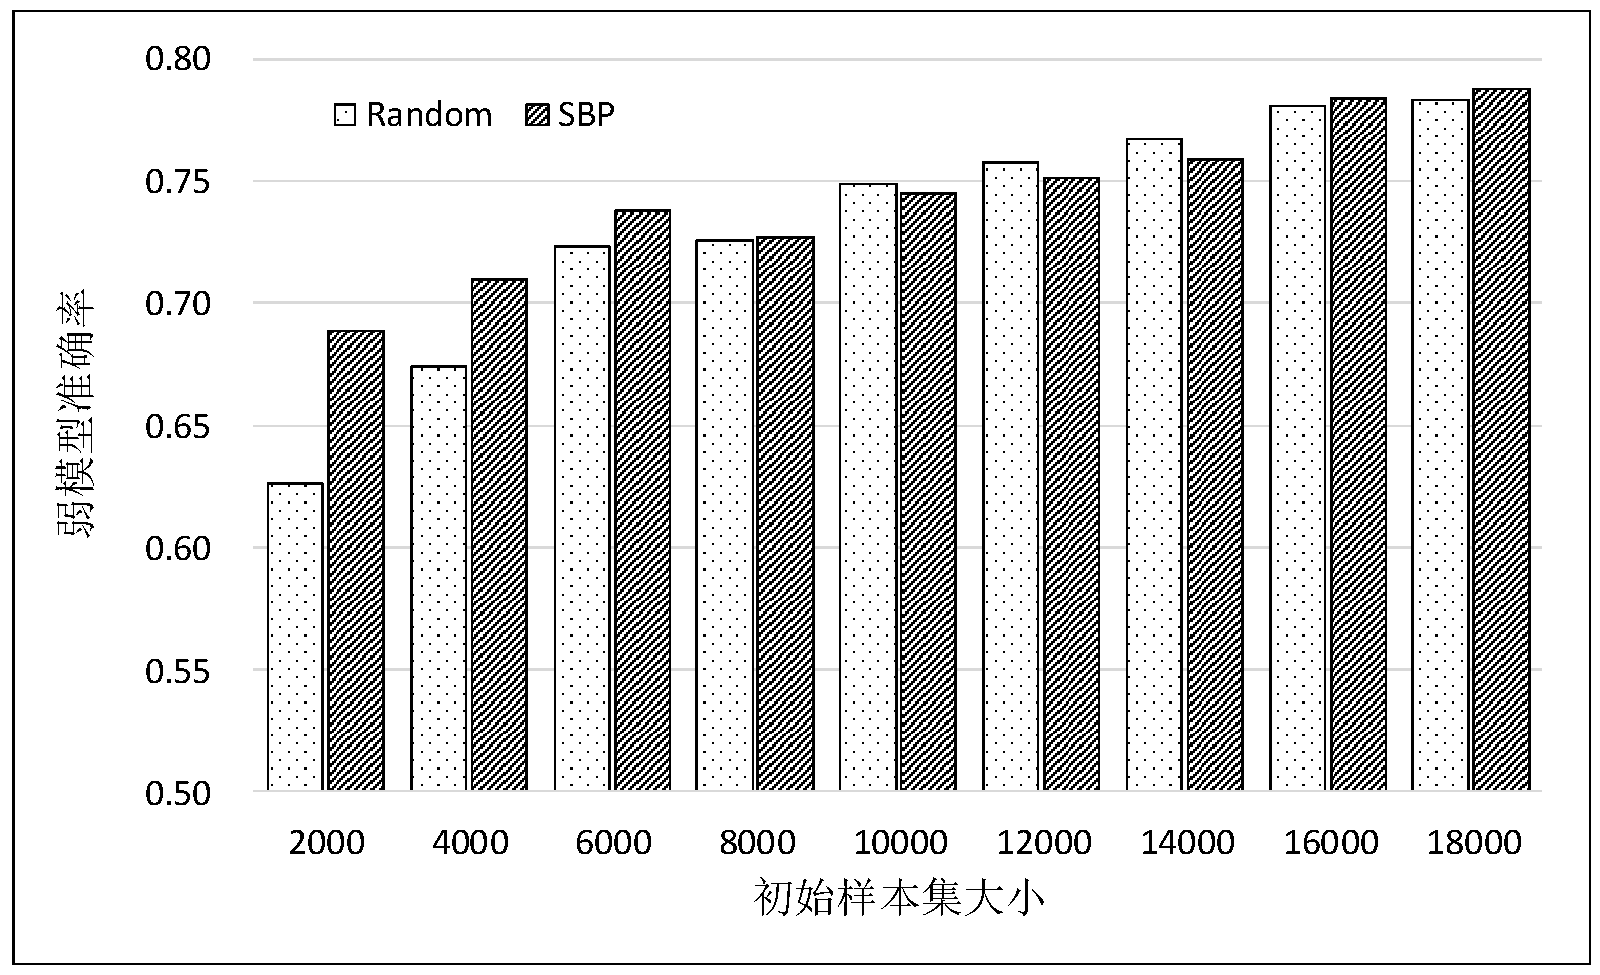
\includegraphics[height=8cm]{resource/surpvised_res1}
	\caption{初始训练样本选择实验结果}
	\label{fig:al_sup_init_result}
\end{figure}

该实验表明,在初始样本集较小的时候,由于样本分布的不均匀特性,随机选择的方法很难选择出能代表整个数据集的样本子集。在实际应用中,用于训练初始模型的初始训练样本集通常较小,使用基于指称项流行度的初始样本选择方法,能有效提升初始模型性能,加快模型在后续训练过程的收敛速度。

\subsection{迭代训练样本选择的实验}
为了验证主动学习方法中不同的样本选择策略对实体链接模型训练的收敛速度的影响,本文在实验环节,对五种不同组合的样本选择策略进行了比较。五种组合如下所示:

(1) Random,初始训练样本和后续迭代训练样本选择都采用随机选择方法,作为基线方法。

(2) Random+Uncertainty,初始训练样本采用随机选择方法,后续迭代训练样本采用基于不确定度的选择方法。

(3) Random+SUP,初始样本采用随机选择方法,后续迭代训练样本采用综合不确定度和流行度的选择方法。

(4) SBP+Uncertainty,初始样本采用基于流行度的选择方法,后续迭代训练样本采用基于不确定度的选择方法。

(5) SBP+SUP,初始样本采用基于流行度的选择方法,后续迭代训练样本采用综合不确定度和流行度的选择方法。

\begin{figure}[!htb]
	\centering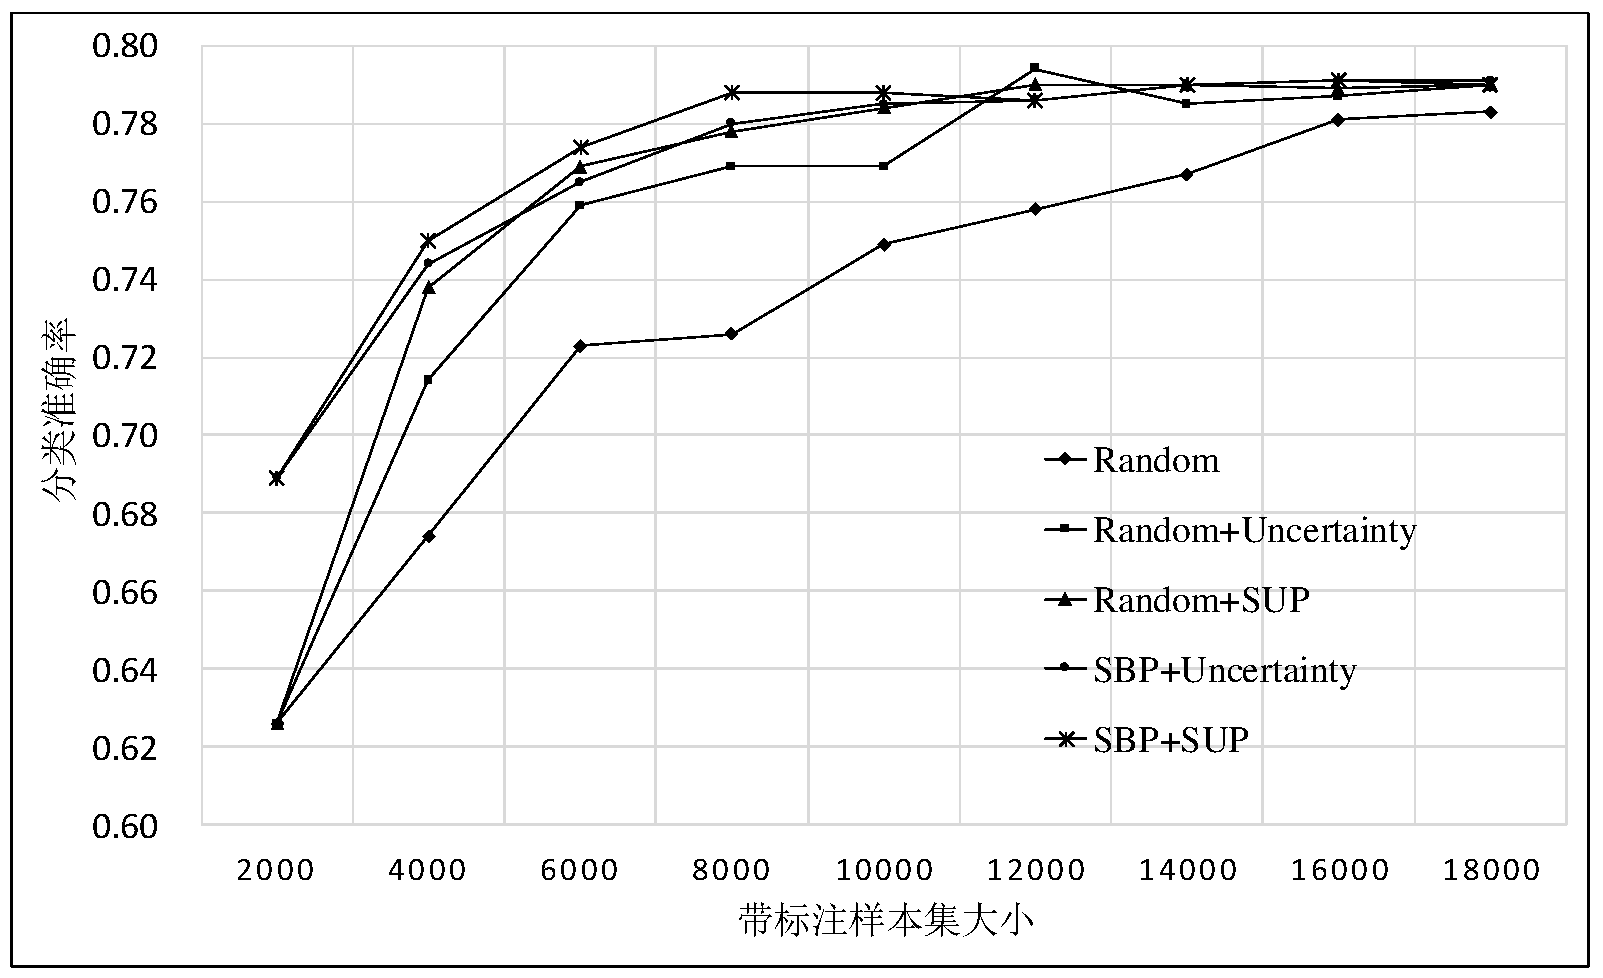
\includegraphics[height=8cm]{resource/surpvised_res2}
	\caption{迭代训练样本选择实验结果}
	\label{fig:al_sup_iter_result}
\end{figure}

从图\ref{fig:al_sup_iter_result}展示的实验结果可以看出,相比随机选择的基线方法,其它四种基于主动学习的样本选择策略对加快模型训练的收敛速度都有显著的提高。证明主动学习方法在实体链接任务中,对减少人工标注样本的工作量确实是有显著效果的。另外,观察曲线走势,综合不确定度和流行度的样本选择方法要优于基于不确定度的样本选择方法,这也验证了基于不确定度的样本选择方法并不能找到最具信息量的样本集,主动学习样本选择过程中需要兼顾不确定度和多样性。

为了量化各种主动学习样本选择策略的表现,采用基于$deficiency$值\cite{schein2007active}的度量方式进行评价,如公式\ref{eq:deficiency}所示。

\begin{equation}\label{eq:deficiency}
Def_n(AL,REF)=\frac{\sum_{t=1}^{n}(acc_n(REF)-acc_t(AL))}{\sum_{t=1}^{n}(acc_n(REF)-acc_t(REF))} \\
\end{equation}

其中,$acc_n(REF)$和$acc_n(AL)$分别表示第$t$轮迭代训练基线方法和主动学习方法训练的模型在测试集上的准确率。主动学习器性能越好,等式分母中$acc_t (AL)$值越大,则等式计算值越小。因此,$Def_n(AL,REF)$越小,主动学习效果越好。

\begin{table}[!htb]
	\caption{主动学习策略结果评价\label{tab:supervised_result2}}
	\centering
	\begin{tabular}{|c|c|c|c|c|}
		\hline
		Random & Random+Uncertainty & Random+SUP & SBP+Uncertainty & SBP+SUP\\
		\hline
		1.000 & 0.552 & 0.369 & 0.274 & \textbf{0.190}\\ 
		\hline
	\end{tabular}
\end{table}

表\ref{tab:supervised_result2}是对主动学习效果的定量分析,无论基于随机的初始样本选择还是基于流行度的初始样本选择,在后续迭代训练中采用基于不确定度和流行度的样本选择算法都能比基于不确定度的样本选择算法得到更快的训练收敛速度。并且采用基于流行度的初始训练样本选择配合综合不确定度和流行度的迭代训练样本选择的策略,$deficiency$值是最低的,性能表现最优。

\section{本章小结}
本章针对实体链接问题,基于主动学习方法,研究了减小人工标注工作量的方法。并且在已有主动学习方法的基础上,针对实体链接任务提出了基于流行度的初始样本选择算法、综合不确定度和流行度的迭代训练样本选择算法。实验结果表明,主动学习方法可以有效地降低实体链接训练集的标注数据,并保持较高的泛化能力。在初始样本集生成阶段,本文提出的选择算法相比随机选择的基线算法初始分类器性能 升了 10.1\%。在主动学习迭代训练阶段,本文 提出的选择算法相比基于不确定度的选择算法$deficiency$值降低了 16.1\%。
%\chapter{基于主动学习的实体链接语料构建}
本章以无监督学习模型辅助实体链接银标准语料的构建,研究主动学习方法在减少人工标注语料数量上的作用。首先介绍基于图的无监督学习的实体链接方法,包括模型使用的特征以及模型对实体链接任务的处理方法。接着,介绍如何使用主动学习方法选择需要人工辅助标注的样本。最后给出实验结果和实验分析。

\section{基于图的协同推断}
构建语料的常用方法是借助已有模型进行辅助构建,本节将首先给出用于辅助标注实体链接语料的基于图的协同推断方法,这是Han等人\cite{CELWTGBM}提出的一种基于无监督学习的实体链接方法。

在例子“Michael Jordan, the Chicago Bulls retired professional basketball player,  starred in the 1996 feature film Space Jam.”中,已有实体链接方法会通过词袋模型计算指称项“Michael Jordan”和目标实体\textit{Michael Jordan}的相似度,例如实体\textit{Michael Jordan}的维基百科页面摘要中包含“Jordan played 15 seasons in the National Basketball Association (NBA)”,可以看出,由于指称项上下文和实体摘要文本的单词完全不相同,该种方式计算所得的相似度为0。但是“Chicago Bulls”和“NBA”之间却是具有很强的语义关联度的。为了解决这种语义的问题,基于图的协同推断方法借助知识库中的相关信息,建立了实体之间的相关联系,在考虑单个指称项与其对应的候选实体之间的相似度的同时,还考虑了在同一个文档中,不同的指称项之间的候选实体的关联度。

\subsection{实体-实体相似度}\label{section:mm_relation}
同一篇文档中的实体之间一般会有相互关联。在处理实体链接任务时,需要通过定量的方式计算两个实体之间的相似度。张涛等人\cite{张涛2015GraphEL}通过知识库(维基百科)中的链接关系计算实体间的相似度。计算过程中考虑到了其他指称项对应的实体,因而也称为全局相似度。

\begin{figure}[!htb]
	\centering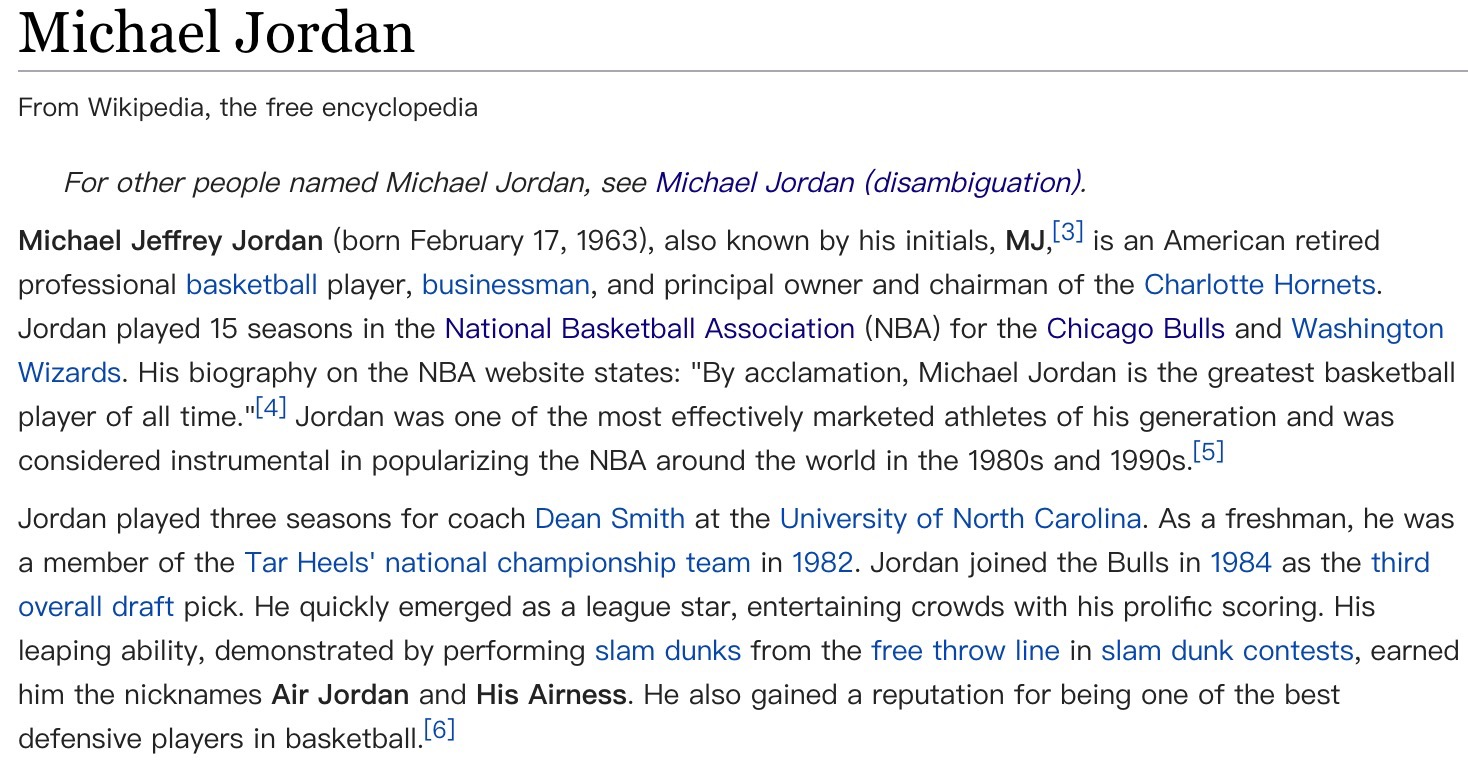
\includegraphics[height=7cm]{resource/jordan_abst}
	\caption{维基百科中\textit{Michael Jordan}的页面}
	\label{fig:jordan_abst}
\end{figure}

图\ref{fig:jordan_abst}是实体\textit{Michael Jordan}在维基百科词条中的部分文本。可以看到,词条文本包含了大量的指向其它实体的链接,例如National Basketball Association、Chicago Bulls、Washington Wizards等。本文通过统计维基百科实体页中的实体链接情况,统计出各个实体在其他实体对应的实体页中被链接的次数,然后计算实体实体之间的相似度,例如,实体$a$和实体$b$之间的相似度可以表示为:

\begin{equation}\label{eq:e_e_relation}
SR(a,b)=1-\frac{\log (\max(|A|,|B|))-\log(|A\cap B|)}{\log(|W|)-\log(\min(|A|,|B|))}
\end{equation}

公式\ref{eq:e_e_relation}中,$A$和$B$分别表示维基百科中对应实体页中包含链接到实体$a$和实体$b$的实体集合。$W$表示维基百科中所有实体的集合。在示例文本中,包含“Michael Jordan”、“Chicago Bulls”、“Space Jam”这三个指称项,其中“Michael Jordan”指向的实体可能是\textit{Michael Jordan},也可能是\textit{Michael B. Jordan}。计算这两个实体和其它两个指称项对应的实体之间的相似度,结果如表\ref{tab:ee_relation_example}所示。

\begin{table}[!htb]
	\caption{实体间相似度例子\label{tab:ee_relation_example}}
	\centering
	\begin{tabular}{|c|c|c|}
		\hline
		 & Space Jam & Chicago\\
		\hline
		Michael Jordan & 0.66 & 0.82\\
		\hline
		Michael B. Jordan & 0.00 & 0.00\\
		\hline
	\end{tabular}
\end{table}

观察该表可以发现,当确定文本中指称项“Chicago Bulls”和“Space Jam”所指向的实体分别是\textit{Chicago Bulls}和\textit{Space Jam}之后,计算\textit{Michael Jordan}与\textit{Chicago Bulls}、\textit{Space Jam}的实体相似度分别是$0.66$和$0.82$,\textit{Michael B. Jordan}与\textit{Chicago Bulls}、\textit{Space Jam}的实体相似度都是$0.00$。由此可以推断,\textit{Michael Jordan}与上下文环境的实体相似度更大,更有可能是指称项“Michael Jordan”对应的目标实体。

\subsection{指称项-实体相似度}\label{section:me_relation}
指称项-实体相似度是指在给定指称项$m$和候选实体$e$后,根据指称项$m$上下文等特征计算得到的和候选实体$e$之间的相似度。计算相似度时,因为只考虑单个指称项,因而也称为局部相似度。

计算指称项-实体相似度需要为指称项的上下文定义一个窗口大小,通过计算该窗口文本和候选实体词条摘要文本的相似度得到指称项-实体相似度。本文参考Pedersen等人\cite{pedersen2005name}的相关研究,将上下文的窗口大小定义为50。

本文采用词袋模型计算指称项-实体相似度,给定指称项$m$和候选实体$e$,指称项-实体相似度如公式\ref{eq:m_m_relation}所示:

\begin{equation}\label{eq:m_m_relation}
CP(m,e)=\frac{m\cdot e}{|m||e|}\\
\end{equation}

其中,$m$和$e$分别是指称项窗口文本和候选实体知识库摘要文本的词向量表示,向量中的每个维度分别是对应单词的TFIDF表示。

\subsection{构建协同推断图}\label{section:ref_graph}
协同推断图的每个节点可以是指称项,也可以是指称项对应的候选实体。图中的边分为两种类型,第一类是指称项节点和候选实体节点之间的边,这类边的权值用指称项-实体相似度表示。第二类是候选实体节点和其它候选实体节点之间的边,这类边的权值用实体-实体相似度表示。由于一个指称项对应的候选实体集包含的候选实体数量可能非常大,那么协同推断图的节点和边的数量可能也会非常大。图的复杂度太高会直接影响后续在图上相关计算的效率,为了解决这个问题,本文对连接边权值较小的候选实体节点和边做了删除处理。

\begin{figure}[!htb]
	\centering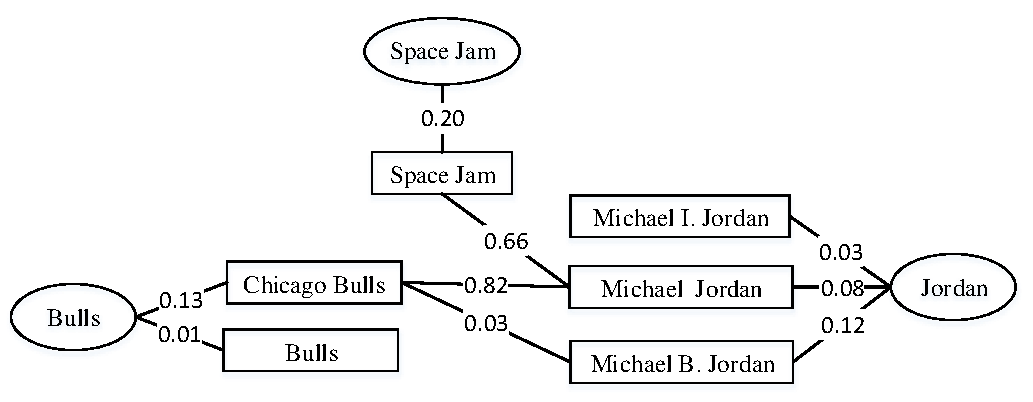
\includegraphics[height=5cm]{resource/EL_Graph}
	\caption{协同推断图示例图}
	\label{fig:el_graph}
\end{figure}

图\ref{fig:el_graph}是实体链接任务中协同推断图的一个例子。图中椭圆边框的节点表示指称项,矩形边框的节点表示指称项对应的候选实体。例如指称项“Jordan”的候选实体包含\textit{Michael I. Jordan}、\textit{Michael Jordan}、\textit{Michael B. Jordan}。指称项“Jordan”与其对应的候选实体之间的边的权值是指称项和实体之间的局部相似度。不同指称项对应的候选实体之间的边为全局相似度,例如指称项“Jordan”对应的候选实体\textit{Michael Jordan}和指称项“Bulls”的候选实体\textit{Chicago Bulls}的实体相似度为0.82。图中并非所有节点都有连接边,这是因为一些边的权值很小,为提高后续计算效率而被删除。

\subsection{协同推断方法}\label{section:collective_infer_method}
构建好协同推断图以后,通过随机行走(Random Walk, RW)算法\cite{tong2006fast}对候选实体的置信度进行推断,选择置信度最高的候选实体作为预测目标实体。

协同推断图中包含$n$个节点($k$个指称项节点和$l$个候选实体节点)。首先需要计算文本中所有指称项在上下文中的重要程度,如公式\ref{eq:m_importance}所示。

\begin{equation}\label{eq:m_importance}
Importance(m)=\frac{tfidf(m)}{\sum_{m\in D} tfidf(m)}\\
\end{equation}

初始证据向量$s$的维度为$k+l$,对$s$的初始化方法如公式\ref{eq:init_evidence}所示。

\begin{equation}\label{eq:init_evidence}
s_i=\left\{
\begin{array}{rcl}
Importance(m)       &      & {\text{节点}i\text{对应指称项}m}\\
0    &      & {\text{节点}i\text{对应候选实体}}
\end{array} \right.
\end{equation}

证据传递矩阵$T$是一个大小为$(k+l)\times (k+l)$的矩阵。该矩阵是一个稀疏矩阵,定义如公式\ref{eq:prob_trans_maze}所示。公式中$E_m$表示指称项$m$对应的候选实体集,$N_e$表示推断图中与实体$e$有边相连的实体集合。

\begin{equation}\label{eq:prob_trans_maze}
T_{ij}=\left\{
\begin{array}{rcl}
\frac{CP(m,e)}{\sum_{e\in E_m} CP(m,e)}       &      & {\text{节点}j\text{对应指称项}m\text{,节点}i\text{对应候选实体}e}\\
\frac{SR(e_i,e_j)}{\sum_{e\in N_{e_j} SR(e_i,e)}}    &      &{\text{节点}j\text{对应候选实体}e_j\text{,节点}i\text{对应候选实体}e_i}\\
0    &      &{\text{其它}}\\
\end{array} \right.
\end{equation}

在实体链接任务中,随机行走算法如算法\ref{algorithm_random_walk}所示。

\floatname{algorithm}{算法}
\renewcommand{\algorithmicrequire}{\textbf{输入:}} % Use Input in the format of Algorithm
\renewcommand{\algorithmicensure}{\textbf{输出:}} % Use Output in the format of Algorithm
\begin{algorithm}[!htb]
	\caption{基于图的协同推断中的随机行走算法}
	\label{algorithm_random_walk}
	\begin{algorithmic}[1] %这个1 表示每一行都显示数字
		\REQUIRE ~ %算法的输入参数:Input
		初始证据向量$s$,证据传递矩阵$T$
		\ENSURE ~ %算法的输出:Output
		图的稳定状态证据向量$r^*$
		\STATE 初始化$r^0=s$
		\REPEAT
		\STATE $r^{t+1}=(1-\lambda)\times T\times r^t + \lambda \times s$\label{random_walk_iter}
		\UNTIL {$r$得到稳定状态或者迭代次数达到上限}\label{random_walk_stop_condition}
		\RETURN $r^*$
	\end{algorithmic}
\end{algorithm}

由于$T$是一个稀疏矩阵,协同推断图中存在一些候选实体节点没有出边,因此算法\ref{algorithm_random_walk}的第\ref{random_walk_iter}行,在随机行走的迭代过程中,加入了证据重分配率参数$\lambda$\footnote{本文通过实验,取$\lambda=0.5$,效果最佳。},这是为了在随机行走过程中以一定概率从起始点重新进行随机行走,解决某些节点无法进行证据传播的问题。参考Hu等人\cite{hu2009understanding}的相关研究,算法第\ref{random_walk_stop_condition}行的迭代次数上限,本文选取的值为100。

以图\ref{fig:el_graph}为例,初始证据向量$s=\left( 0.41,0.33,0.26,0,0,0,0,0,0\right)^T $,$r^0=s$。随机行走过程第1次迭代如公式\ref{eq:random_walk_iter1}所示。

\begin{equation}\label{eq:random_walk_iter1}
\left(
\begin{matrix}
0.21\\
0.17\\
0.13\\
0.03\\
0.07\\
0.11\\
0.15\\
0.01\\
0.13\\
\end{matrix}
\right)
=.5\times
\left(
\begin{matrix}
0 & 0 & 0 & 0 & 0 & 0 & 0 & 0 & 0\\
0 & 0 & 0 & 0 & 0 & 0 & 0 & 0 & 0\\
0 & 0 & 0 & 0 & 0 & 0 & 0 & 0 & 0\\
0.13 & 0 & 0 & 0 & 0 & 0 & 0 & 0 & 0\\
0.35 & 0 & 0 & 0 & 0 & 0 & 0.96 & 0 & 0\\
0.52 & 0 & 0 & 0 & 0 & 0 & 0.04 & 0 & 0\\
0 & 0.92 & 0 & 0 & 0.55 & 1 & 0 & 0 & 0\\
0 & 0.08 & 0 & 0 & 0 & 0 & 0 & 0 & 0\\
0 & 0 & 1 & 0 & 0.45 & 0 & 0 & 0 & 0\\
\end{matrix}
\right)\times
\left(
\begin{matrix}
0.41\\
0.33\\
0.26\\
0\\
0\\
0\\
0\\
0\\
0\\
\end{matrix}
\right)+
.5\times
\left(
\begin{matrix}
0.41\\
0.33\\
0.26\\
0\\
0\\
0\\
0\\
0\\
0\\
\end{matrix}
\right)
\end{equation}

在完成第100轮随机行走迭代过程后,达到了稳定状态下,最后一轮迭代如公式\ref{eq:random_walk_iter100}所示。

\begin{equation}\label{eq:random_walk_iter100}
\left(
\begin{matrix}
0.21\\
0.17\\
0.13\\
0.01\\
0.10\\
0.06\\
0.13\\
0.01\\
0.09\\
\end{matrix}
\right)
=.5\times
\left(
\begin{matrix}
0 & 0 & 0 & 0 & 0 & 0 & 0 & 0 & 0\\
0 & 0 & 0 & 0 & 0 & 0 & 0 & 0 & 0\\
0 & 0 & 0 & 0 & 0 & 0 & 0 & 0 & 0\\
0.13 & 0 & 0 & 0 & 0 & 0 & 0 & 0 & 0\\
0.35 & 0 & 0 & 0 & 0 & 0 & 0.96 & 0 & 0\\
0.52 & 0 & 0 & 0 & 0 & 0 & 0.04 & 0 & 0\\
0 & 0.92 & 0 & 0 & 0.55 & 1 & 0 & 0 & 0\\
0 & 0.08 & 0 & 0 & 0 & 0 & 0 & 0 & 0\\
0 & 0 & 1 & 0 & 0.45 & 0 & 0 & 0 & 0\\
\end{matrix}
\right)\times
\left(
\begin{matrix}
0.21\\
0.17\\
0.13\\
0.01\\
0.10\\
0.06\\
0.13\\
0.01\\
0.09\\
\end{matrix}
\right)+
.5\times
\left(
\begin{matrix}
0.41\\
0.33\\
0.26\\
0\\
0\\
0\\
0\\
0\\
0\\
\end{matrix}
\right)
\end{equation}

对于给定的指称项$m$,基于图的协同推断方法用公式\ref{eq:collective_inference}计算$m$对应的预测目标实体。其中$r(e)$是随机行走达到稳定状态后,候选实体$e$通过图推断后得到的评分,与局部相似度$CP(m,e)$相乘后得到综合评分,并取指称项$m$对应的候选实体集中,综合评分最高的候选实体作为$m$的预测目标实体。

\begin{equation}\label{eq:collective_inference}
m.e^*=\argmax_e CP(m,e)\times r(e)
\end{equation}

\begin{table}[!htb]
	\caption{主动学习策略结果评价\label{tab:el_graph_score}}
	\centering
	\begin{tabular}{|c|c|c|c|}
		\hline
		\textbf{候选实体} & \textbf{Michael I. Jordan} & \textbf{Michael Jordan} & \textbf{Michael B. Jordan}\\
		\hline
		$r(e)$ & 0.01 & 0.10 & 0.06\\
		\hline
		\textbf{候选实体} & \textbf{Chicago Bulls} & \textbf{Bulls} & \textbf{Space Jam}\\
		\hline
		$r(e)$ & 0.13 & 0.01 & 0.09\\
		\hline
	\end{tabular}
\end{table}

表\ref{tab:el_graph_score}给出了本节的例子中,各个候选实体在随机行走达到稳定状态后的推断评分。通过观察可以发现,经过协同推断进程后,候选实体\textit{Michael Jordan}、\textit{Chicago Bulls}、\textit{Space Jam}是在其对应的指称项的候选实体集里面推断评分最高的,通过公式\ref{eq:collective_inference}计算得到的综合评分也是最高的,验证了基于图的协同推断方法的有效性。

\section{银标准语料构建方法}
银标准语料即存在错误标注,但不会对模型训练产生很大影响的语料。在成本有限的情况下,提高银标准语料质量对模型训练有重要意义。虽然Han等人\cite{CELWTGBM}通过实验证明了基于图的协同推断方法是目前性能较好的实体链接方法,但是该方法在本文所使用的数据集上仅能达到73.3\%的正确率。其在正确率上距离高质量银标准语料还有一定差距。常用的方法是人工对部分未标注样本进行标注,然后通过已标注样本对未标注样本进行证据传播,从而提高其它未标注样本的预测精度。

在人工标注并证据传播的过程中,有以下两个关键问题:

(1)如何从未标注指称项样本中选择需要交由人工标注的待标注样本。

(2)对指称项对应的目标实体进行标注以后,如何影响其它未标注样本的目标实体预测。

本文将在以下两节分别介绍待标注指称项的选择方法和已标注指称项的证据传播方法。

\subsection{待标注指称项选择方法}\label{section:anno_select}
以下是四种待标注指称项选择方法,其中第一种采用顺序选择方法,后三种都是基于主动学习的选择方法。

\subsubsection{顺序指称项选择法}
该方法是一种基线方法。对一篇文档$D$中的所有指称项$M=\{m_1,m_2,...,m_n\}$,按照指称项出现的先后顺序对指称项进行标注。

该方法的优点在于实现简单,并且顺序标注符合人的标注习惯。该方法的缺点是,当实体链接模型性能较高的时候,提交人工标注的指称项有很大概率已经被正确预测,增加人工标注的工作量,标注效率较低。

\subsubsection{最大不确定度的指称项选择法}\label{section:margin_select}
该方法利用基于间隔的主动学习方法对待标注指称项进行了选择。对于给定指称项$m$及其候选实体集合$E_m$,对$E_m$中的每个候选实体$e$的综合评分做归一化处理,得到候选实体$e$是目标实体的置信度,如公式\ref{eq:el_graph_prob}所示。

\begin{equation}\label{eq:el_graph_prob}
P(e|m)=\frac{CP(m,e)\times r(e)}{\sum_{e\in E_m}CP(m,e)\times r(e)}
\end{equation}

通过公式\ref{eq:el_graph_confidence}计算指称项$m$的候选实体中综合评分最高的两个候选实体的置信度的差的绝对值,以此作为指称项$m$被正确链接的置信度。
\begin{align}\label{eq:el_graph_confidence}
\begin{aligned}
	Confidence(m)&=P(e^{*1}|m)-P(e^{*2}|m)\\
	\text{其中,\quad\quad\quad\quad\quad\quad\quad\quad\quad\quad\quad}&\text{\quad\quad\quad\quad\quad\quad\quad\quad\quad\quad\quad\quad\quad\quad\quad\quad\quad}\\
	e^{*1}&=\argmax_{e_i\in E_m}P(e_i|m)\\
	e^{*2}&=\argmax_{e_i\in E_m \setminus e^{*1}}P(e_i|m)
\end{aligned}
\end{align}

得到指称项$m$被正确链接的置信度以后,通过公式\ref{eq:el_graph_uncertainty}计算指称项$m$链接的不确定度。
\begin{equation}\label{eq:el_graph_uncertainty}
Uncertainty(m)=1-Confidence(m)
\end{equation}

链接不确定度越大的指称项,预测标注错误的可能性越大。因此,在每一轮待标注样本选择过程中,需要选择链接不确定度最大的指称项交由人工标注,通过这种方式尽可能找出错误预测的指称项,从而提高人工标注的效率。

\subsubsection{基于同名指称项的最大标注回报选择法}
该方法在利用主动学习方法选择待标注样本的过程中,不仅考虑到了样本的不确定度,同时也考虑到了样本的代表性。在同一篇文档中,相同的指称项可能出现多次,这些指称项很可能指向同一个实体。对这些指称项中的某一个指称项做人工标注,可以提高其它指称项预测的正确率。这里,对指称项$m$进行标注的回报率进行评估时,评估结果由与$m$同名的指称项集合$M_m=\{m^{'}|Name_m=Name_{m^{'}}\}$中的所有指称项共同确定,如公式\ref{eq:dupName_uncartainty}所示。

\begin{equation}\label{eq:dupName_uncartainty}
Reward(M_m)=\sum_{m^{'}\in M_m} {Uncertainty(m^{'})}
\end{equation}

从公式中可以直观地看出,同一文档中,同名指称项出现的次数越多,各个指称项链接的不确定度越大,则对指称项进行人工标注的回报率越大。对$Reward(M_m)$值最大的指称项集合$M_m$中的某个指称项进行人工标注,理论上对语料库实体链接预测正确率的提升效果最大。

\subsubsection{基于相似指称项的最大标注回报选择法}
存在一些指称项集合,它们存在共指关系,但是它们名字的字符串并不是严格相等的,可能是缩写、别名等其它形式。例如在同一篇文档中,指称项“Microsoft”和指称项“MS”可能就是全名和缩写的关系,它们所指向的实体是相同的。基于字符串完全匹配的方法的缺点是无法利用这类指称项之间的共指关系。

为了克服上述缺点,本文提出了基于相似指称项的最大标注回报选择方法。本文通过知识库相关信息抽取得到候选实体词典,然后借助候选实体词典,根据指称项对应的候选实体集计算不同指称项之间的语义相似度。

\begin{equation}\label{eq:mention_semi}
MS(m_1,m_2)=\frac{|E_{m_1}\cap E_{m_2}|}{\min(|E_{m_1}|,|E_{m_2}|)+0.1}
\end{equation}

公式\ref{eq:mention_semi}是指称项$m_1$和指称项$m_2$之间语义相似度的计算方法。该公式的假设是,相同或相似的指称项,对应的候选实体集相似度也应该会更高。在极端情况下,两个相同的指称项,候选实体集完全相同,指称项之间的语义相似度为1。相反,完全不相关的指称项,对应的候选实体集交集为空,则指称项之间的语义相似度为0。

因此,在评估指称项$m$的标注回报率时,评估结果由与$m$相似的指称项集合$M_m=\{m^{'}|MS(m,m^{'})>=\alpha\}$(公式中的$\alpha$通过实验获得,本文取值为0.8)中的所有指称项共同确定,计算方式与公式\ref{eq:dupName_uncartainty}相同,也是由指称项集合$M_m$中的所有指称项链接不确定度的和得到。

同样地,选择需要人工标注的指称项时,也是需要从$Reward(M_m)$最大的指称项集合中取出一个指称项进行标注,这里从集合中选取的原则是选择不确定度最大的指称项。

\subsection{已标注指称项证据传播方法}\label{section:anno_propagate}
同一篇文档会包含多个指称项,一方面,这些指称项通常会有相互关联的关系,例如同一篇文档中既包含“Jordan”这个指称项,又包含“Bulls”这个指称项。如果人工标注“Jordan”指向\textit{Michael Jordan}这个实体,那么“Bulls”则很可能指向\textit{Chicago Bulls}这个实体。另一方面,采用基于同名指称项的最大标注回报选择法和基于相似指称项的最大标注回报选择法时,经过人工标注的指称项会对文档中的其它未标注指称项的目标实体预测产生一定的影响。

在同一篇文档中,相同或者相似的指称项可能会出现多次,例如出现多个“Jordan”指称项,当人工标注其中一个“Jordan”指向\textit{Michael Jordan}这个实体,那么其它“Jordan”指称项很可能也指向\textit{Michael Jordan}这个实体。另外还需要考虑到不同字符串表示的指称项可能存在共指关系,即它们可能指向同一个实体,例如指称项“Jordan”和指称项“Michael Jordan”如果出现在同一篇文档中,则它们也很可能指向同一个实体\textit{Michael Jordan}。

\subsubsection {图的迭代推断}
当标注者标注指称项$m$指向实体$e$以后,需要对协同推断图做以下处理。首先,需要删除指称项$m$对应的候选实体集$E_m$中除目标实体$e$以外的其他候选实体节点。然后删除与被移除节点相连的边。

\begin{figure}[!htb]
	\centering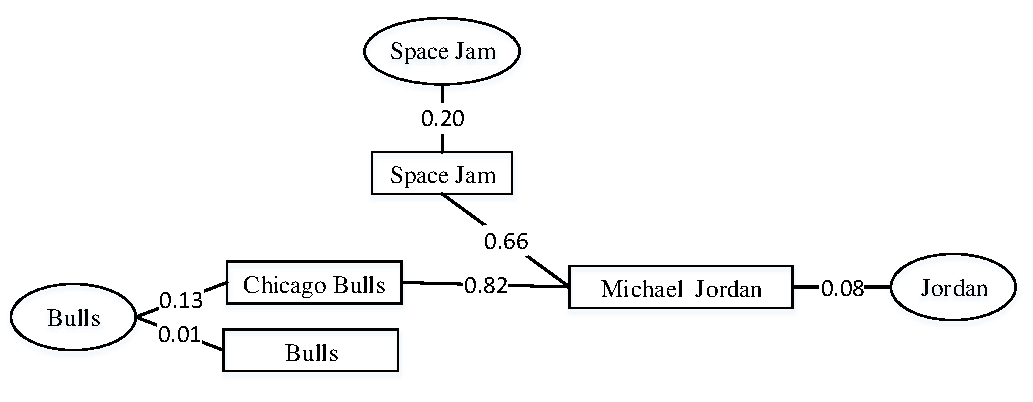
\includegraphics[height=5cm]{resource/EL_Graph_modify}
	\caption{协同推断图示例图}
	\label{fig:el_graph_modify}
\end{figure}

例如将指称项“Jordan”进行人工标注指向\textit{Michael Jordan}实体,改动后的协同推断图如图\ref{fig:el_graph_modify}所示。图中指称项“Jordan”对应的候选实体集中\textit{Michael I. Jordan}实体和\textit{Michael B. Jordan}实体对应的节点被删除,指称项“Jordan”连接到实体\textit{Michael I. Jordan}和实体\textit{Michael B. Jordan}的边被删除,另外,实体\textit{Michael I. Jordan}和实体\textit{Michael B. Jordan}节点连接到其它实体节点的边也被删除。
	
由于经过人工标注以后协同推断图发生了变化,因此对应到协同推断过程,需要根据改动以后的协同推断图对初始证据向量$s$和证据传递矩阵$T$进行改动。改动后的初始证据向量$s$和证据传递矩阵$T$如分别如公式\ref{eq:s_modify}和公式\ref{eq:T_modify}所示。
	
\begin{equation}\label{eq:s_modify}
	s=\left(0.41,0.33,0.26,0,0,0,0\right)^T
\end{equation}
	
\begin{equation}\label{eq:T_modify}
	T=
	\left(
	\begin{matrix}
	0 & 0 & 0 & 0 & 0 & 0 & 0\\
	0 & 0 & 0 & 0 & 0 & 0 & 0\\
	0 & 0 & 0 & 0 & 0 & 0 & 0\\
	1 & 0 & 0 & 0 & 1 & 0 & 0\\
	0 & 0.92 & 0 & 0.55 & 0 & 0 & 0\\
	0 & 0.08 & 0 & 0 & 0 & 0 & 0\\
	0 & 0 & 1 & 0.45 & 0 & 0 & 0\\
	\end{matrix}
	\right)
\end{equation}
	
通过观察可以发现,由于删除了部分节点,$s$和$T$的维度发生了变化,另外协同推断图边的权值变化也引起了$T$中部分值的变化。后续推断过程按照第\ref{section:collective_infer_method}节描述的方法进行即可。

\subsubsection{标注证据传播}
当人工标注指称项$m$指向目标实体$e$以后,需要将标注结果传播到同一篇文档中的其他可能共指的指称项。本文采用了两种标注证据传播方法:基于字符串完全匹配的标注证据传播方法和基于相似指称项的标注证据传播方法。

(1)基于字符串完全匹配的标注证据传播

当人工标注文档$D$中的某一个指称项$m$指向目标实体$e$以后,在文档$D$中搜索与指称项$m$名字完全相同的未标注指称项集合$M_m=\{m^{'}|Name_m=Name_{m^{'}}\}$。然后需要调整证据传递矩阵$T$中所有$m^{'}\in M_m$的指称项节点连接到其对应候选实体节点的边的权值,如公式\ref{eq:T_dupName}所示。
	
\begin{equation}\label{eq:T_dupName}
	T_{ij}=\left\{
	\begin{array}{rcl}
	1      &      & {\text{节点}j\text{对应指称项}m^{'}\text{,节点}i\text{对应实体}e}\\
	0    &      &{\text{节点}j\text{对应指称项}m^{'}\text{,节点}i\text{对应除}e\text{以外的其它实体}}\\
	\end{array} \right.
\end{equation}

(2)基于相似指称项的标注证据传播
	
当人工标注文档$D$中的某一个指称项$m$指向目标实体$e$以后,在文档$D$中搜索与指称项$m$语义相似度不小于$\alpha$的未标注指称项集合$M_m=\{m^{'}|MS(m,m^{'})>=\alpha\}$。同时依然要对证据传递矩阵$T$做调整,按照公式\ref{eq:T_simiName1}对所有$m^{'}\in M_m$的指称项节点连接到实体节点的边的权值做调整。
	
\begin{equation}\label{eq:T_simiName1}
	T_{ij}=\left\{
	\begin{array}{rcl}
	MS(m,m^{'})\times T_{ij}      &      & {\text{节点}j\text{对应指称项}m^{'}\text{,}}\\
	&	&{\text{节点}i\text{对应实体}e}\\
	(1-MS(m,m^{'}))\times T_{ij}    &      &{\text{节点}j\text{对应指称项}m^{'}\text{,}}\\
	&	&{\text{节点}i\text{对应除}e\text{以外的其它实体}}\\
	\end{array} \right.
\end{equation}
	
调整权值之后,还需要对所有指向指称项的节点$j$通过公式\ref{eq:T_simiName2}对权值做归一化处理。
	
\begin{equation}\label{eq:T_simiName2}
	T_{ij}=\frac{T_{ij}}{\sum_{k} {T_{kj}}}
\end{equation}

\section{实验结果与分析}
\subsection{实验环境}
同\ref{section:dev_env}节。

\subsection{实验数据集}
数据集同\ref{section:dataset}节,因为本章实验内容为实体链接银标准语料的辅助标注,因此不需要将数据集划分为训练集和测试集。

\subsection{实验设置}\label{section:anno_set}
本章研究主动学习方法在实体链接银标准语料构建中的作用,并验证本文提出的融合证据传播的主动学习方法对减少人工标注样本工作量的效果。实验过程中不直接使用Aida数据集的标注结果,而只使用模型选择的待标注样本的标注结果。本章设计了以下六个对比实验:

(1) 以顺序标注方法作为基线方法,评价标注过程中,语料中指称项链接的正确率的变化,同下列基于主动学习的标注方法做比较。

(2)以最大不确定度的指称项选择法选择待标注指称项,在标注证据传播过程中,不对当前标注结果进行传播。

(3))以最大不确定度的指称项选择法选择待标注指称项,在标注证据传播过程中,基于字符串完全匹配对当前标注结果进行传播。

(4) 以最大不确定度的指称项选择法选择待标注指称项,在标注证据传播过程中,基于相似指称项对当前标注结果进行传播。

(5)以基于同名指称项的最大标注回报选择法选择待标注指称项,在标注证据传播过程中,基于字符串完全匹配对当前标注结果进行传播。

(6)以基于相似指称项的最大标注回报选择法选择待标注指称项,在标注证据传播过程中,基于相似指称项对当前标注结果进行传播。

\subsection{实验结果与分析}
\begin{figure}[!htb]
	\centering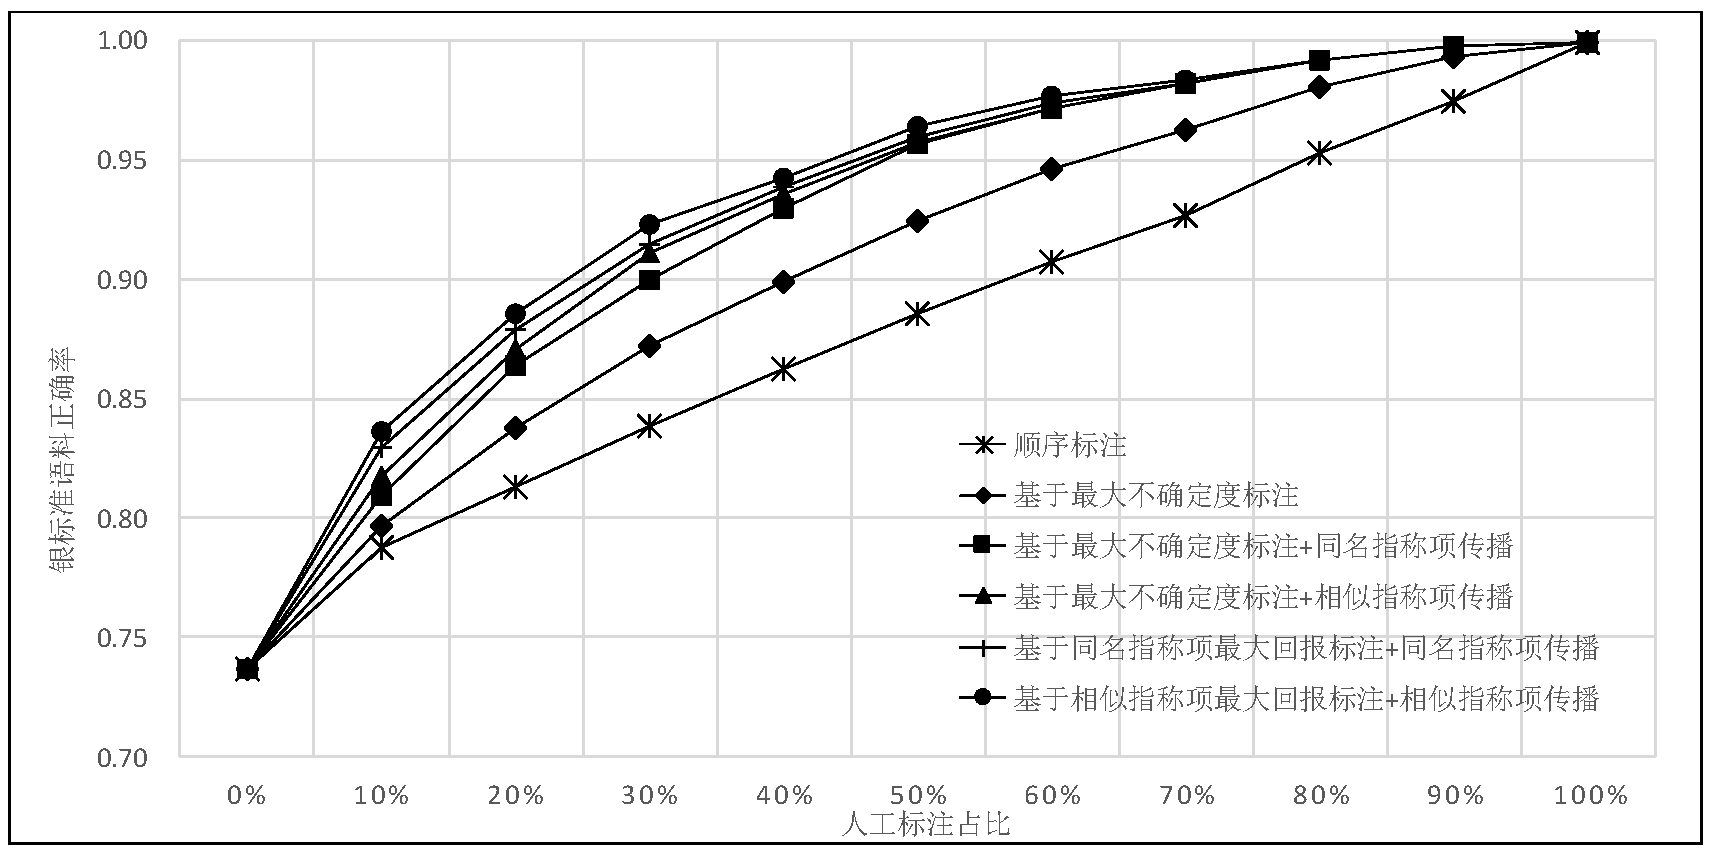
\includegraphics[height=8cm]{resource/anno_result}
	\caption{银标准语料库构建实验结果}
	\label{fig:anno_result}
\end{figure}

本文实验环节测试了上述六种标注方式在数据集上的标注效果。如图\ref{fig:anno_result}所示。顺序标注并且没有对标注证据进行传播的方法,标注效率是最低的。以最大不确定度的指称项选择法选择待标注指称项,在不进行标注证据传播的情况下,标注效率明显优于顺序标注的方式。这是因为该基于主动学习的方法能够有效搜索出预标注不确定度大的样本,保证交由人工标注的样本很可能是预标注错误的样本,从而提高标注效率,并且这一假设通过实验得到了证明。

以最大不确定度的指称项选择法选择待标注指称项,并基于同名指称项和基于相似指称项的方式对当前标注结果进行标注证据传播,观察曲线可以发现,相比于不对标注证据传播的方式,标注效率得到了显著提升,并且基于相似指称项的方式优于基于字符串完全匹配的方式。这是因为,同一文档中相同指称存在多次出现的情况,基于同名指称项的标注证据传播能利用一次标注提高多个未标注指称项的链接正确率。另外,基于相似指称项的证据传播方式能将标注结果传播到存在共指关系的未标注指称项,因此比基于同名指称项的标注证据传播方法性能更好。实验证明,在实体链接银标准语料标注任务中,融合标注证据传播,对提升主动学习方法的性能有显著的效果。

在待标注样本选择阶段,基于同名指称的最大标注回报选择法和基于相似指称的最大标注回报选择法,相比最大不确定度的指称项选择法,标注效率得到提升。提升的原因是,在样本选择的阶段,不仅考虑到单个指称项的预测链接不确定度,还考虑了标注该指称项对文档中其它存在共指关系的指称的影响。

综合分析实验结果数据,在仅标注50\%的指称项时,顺序标注的方式只能将语料库标注正确率提升到88.6\%,而以基于相似指称的最大标注回报选择法选择待标注指称项,在标注证据传播过程中,基于相似指称项对当前标注结果进行传播的方法,标注正确率提升到了96.4\%。

\section{本章小结}
本章介绍了一种基于主动学习的实体链接银标准语料库构建方法。并且,本文基于实体链接任务的特点,对已有的主动学习方法进行了改进,包括引入了基于标注回报率待标注样本选择的评价方式,以及加入了标注样本的证据传播方法,提升了主动学习方法的性能。在本章实验环节,本文对提出的这些方法进行了验证,并分析了实验结果。

\chapter{总结与展望}
\section{总结}
本文为辅助解答高考地理题所尝试的工作,主要解决了在辅助解答地理高考题过程中的两个问题,第一个是缺乏高质量的地理核心知识库,第二个是地理问题表达多样而导致的问理解困难问题。

为解决缺乏高质量的地理核心知识库的问题,本文以高中地理教科书和北京市十年高考地理试题为知识源,通过自底向顶的本体构建思想,先从十年高考题中提炼出地理核心考点,然后去地理教材中寻找可以解答核心考点的核心地理知识,以地理教科书中的知识组织框架为大体的本体知识层次组织,最后通过描述能力很强的本体语言OWL DL表示地理核心知识,得到高质量、高度结构化的地理本体CGeoOnt。同时,本文还将863项目组以百度百科自动构建的中文地理本体Clinga与CGeoOnt融合得到目前中文地理领域规模最大、质量最高的地理本体知识库,用于辅助地理高考解题。

为解决地理问题表达多样而导致的问理解困难问题,本文以 Clinga、CGeoOnt 为中文地理核心知识库,构建了一个对问题适应性很强的问答系统。该问答系统以 Attention-based Bi-LSTM 为问答模型,分别用两个共享参数的 Bi-LSTM 网络来表示问题和答案。同时,答案的表示结合答案序列对问题的注意力权重,模型使用有标记的问答对做训练,在从 web收集到的多样性的地理问题数据集上,问答指标 MRR、Accuracy@N 分别达到 0.834、0.872的好结果, 当一个问题以不同方式提问时,本文模型同样具有很好的适应性。

本文构建的问答系统致力于辅助解答高考地理题,对于单实体单关系的地理问题,即使该问题提问方式形式多样,实验表明本系统仍可以比较好的解决,因此对于解答高考地理题有一定的实用价值。

\section{未来展望}
本文构建地理本体CGeoOnt采用的是人工构建的方式,从整体来看虽然构建的本体质量比较高,但是总体时间花费过大,六人标注团队一年半的时间仅仅标注了两万多条。因此,可以尝试使用自动或者半自动加人工的方式来构建地理本体,并且开发合适的地理知识自动或者半自动标注工具,提高地理标注效率。

再者,对于本文构建的地理知识库问答系统,从模型上看,对于答案的表示,除了本文结合问题中词级别的注意力机制,模型还可以结合地理题本身的特征,如地理问题答案类型、答案关系等,或者还可以结合知识库本体本身丰富的语义特征,将实体的上下文类别语义信息添加到问题、 答案的表示中,从这些方面更加完善地对问题、 答案进行表示,从而提升问答的性能。



\acknowledgement
时光匆匆而逝,我的硕士三年研究生生活即将结束。回首这三年,心中倍感充实。我要感谢我的母校,我庆幸我是一名东大的学子,学校浓厚的学术氛围和舒适的学习环境将令我终生难忘。

首先我要感谢我的导师高志强教授。他在忙碌的教学和科研工作中挤出时间来审查我的开题报告,修改我的论文,是高老师的意见和指导帮助我顺利完成了研究课题。此外,从我进入实验室起,高老师严谨细致、一丝不苟的学术作风也深深地影响着我。同时,也感谢实验室的所有同门朱曼、刘倩、鲁廷明、全志斌、归耀城、李雪莲、吕永涛、王辰、倪朝曦、潘敬敏、司马强、王煜、王李荣、余云秀、张赏、刘金晶、范云龙、李斌、刘延栋、汪文涛、衣克买提等,尤其是鲁廷明师兄、全志斌师兄、余云秀师妹,他们在我的研究和论文上提出了诸多宝贵的意见,并在精神上给予我诸多鼓励,使我受益良多。

感谢我在东大相识的所有伙伴温潇、罗鸿飞等,你们为我的校园生活带来了欢乐与感动。感谢我的室友们在日常生活中对我的关心。感谢所有在学习与项目中与我共同奋斗过的朋友,你们不仅让我体会到了成功的喜悦,也收获了真挚的友情。也许在不久的将来我们会天各一方,但是我会永远记住你们,我的伙伴们。

最后,我要感谢我的父母,让我在人生漫漫长路中有了厚实的依靠。养育之恩,无以回报,在未来的日子里,我会更加努力学习与工作,不辜负父母对我的殷切期望。

\quad

\quad

\rightline{张赏}
\rightline{2018年5月于南京}

\thesisbib{seuthesix}


\appendix

%\resume{作者攻读硕士学位期间的研究成果}
%\begin{flushleft}
%{\bfseries \large 发表的论文}\\ \relax
%[1] 第一作者,“灵犀一指:理论与应用”, 武侠学报,
%2015年5月。\\
%\end{flushleft}


\end{document}